\documentclass[10pt,a4paper]{article}

% --- Paquetes de configuración regional y tipografía ---
\usepackage[utf8]{inputenc}
\usepackage[T1]{fontenc}
\usepackage[spanish,es-tabla,es-noshorthands]{babel}
\usepackage{lmodern}
\usepackage{microtype}

% --- Geometría y márgenes optimizados para informe técnico formal ---
\usepackage[a4paper,top=1.6cm,bottom=1.6cm,left=1.5cm,right=1.5cm,headheight=13pt,footskip=18pt]{geometry}

% --- Elementos gráficos y tablas ---
\usepackage{graphicx}
\graphicspath{{images/}{capturas/}{./}}
\usepackage{xcolor}
\usepackage{booktabs}
\usepackage{tabularx}
\usepackage{colortbl}
\usepackage{float}
\usepackage{caption}
\usepackage{subcaption}
\usepackage{amsmath,amssymb}
\usepackage{tikz}
\usetikzlibrary{shapes.geometric, arrows.meta, positioning, fit, backgrounds, babel}

% --- Espaciados compactos y legibles ---
\setlength{\parskip}{1.8pt plus 0.6pt minus 0.4pt}
\setlength{\intextsep}{3pt plus 1pt minus 1pt}
\setlength{\textfloatsep}{4pt plus 1pt minus 1pt}
\setlength{\floatsep}{3pt plus 1pt minus 1pt}

% --- Estilo de encabezados y pies de página ---
\usepackage{fancyhdr}
\usepackage{lastpage}
\usepackage{titlesec}
\usepackage{enumitem}
\setlist{topsep=1.5pt, itemsep=1.0pt, parsep=0pt, partopsep=0pt}
\renewcommand{\arraystretch}{0.96}

% --- Cajas estilizadas y código ---
\usepackage{tcolorbox}
\tcbuselibrary{skins,breakable,listings}
\usepackage{listings}
\usepackage{multicol}

% --- Hipervínculos ---
\usepackage{xurl}
\usepackage{hyperref}

% --- Definición de Paleta de Colores Institucional UNC / FCEFyN ---
\definecolor{uncblue}{RGB}{10, 48, 92}        % Azul Institucional FCEFyN
\definecolor{primary}{RGB}{18, 52, 86}         % Azul oscuro principal
\definecolor{accentteal}{RGB}{0, 136, 145}     % Teal acento
\definecolor{darkslate}{RGB}{33, 37, 41}       % Texto principal
\definecolor{termbg}{RGB}{17, 24, 39}          % Fondo terminal oscuro (slate 900)
\definecolor{termfg}{RGB}{243, 244, 246}       % Texto terminal blanco nítido
\definecolor{boxbg}{RGB}{248, 250, 252}        % Fondo cajas
\definecolor{boxborder}{RGB}{203, 213, 225}    % Borde cajas
\definecolor{tableheader}{RGB}{226, 232, 240}  % Fondo encabezado tablas
\definecolor{rowalt}{RGB}{248, 250, 252}       % Filas alternas
\definecolor{notebg}{RGB}{239, 246, 255}       % Fondo notas
\definecolor{noteborder}{RGB}{59, 130, 246}    % Borde notas
\definecolor{missingbg}{RGB}{254, 242, 242}     % Fondo captura faltante (rojo suave)
\definecolor{missingborder}{RGB}{239, 68, 68}   % Borde captura faltante (rojo)
\definecolor{codecomment}{RGB}{100, 116, 139}  % Comentarios código
\definecolor{codekeyword}{RGB}{14, 116, 144}   % Keywords C/Bash

% --- Configuración de Hipervínculos ---
\hypersetup{
    colorlinks=true,
    linkcolor=uncblue,
    citecolor=uncblue,
    urlcolor=accentteal,
    pdftitle={Informe Técnico — TP3: Sector en Producción NEXUS-9},
    pdfauthor={Grupo Infostealer - FCEFyN UNC},
    pdfsubject={Sistemas Operativos I - Trabajo Práctico Nro 3}
}

% --- Configuración de Encabezados y Pies de Página ---
\pagestyle{fancy}
\fancyhf{}
\fancyhead[L]{\footnotesize\scshape\color{primary}Sistemas Operativos I — TP N$^\circ$ 3: Sector en Producción}
\fancyhead[R]{\footnotesize\scshape\color{uncblue}Capítulo 3 · Sistema Publicado, Protegido y Recuperable}
\fancyfoot[L]{\scriptsize\color{darkslate!70}FCEFyN — Universidad Nacional de Córdoba}
\fancyfoot[R]{\footnotesize\bfseries\color{primary}Página \thepage\ de \pageref{LastPage}}
\renewcommand{\headrulewidth}{0.5pt}
\renewcommand{\footrulewidth}{0.3pt}

% --- Configuración de Títulos de Sección Compactos ---
\titleformat{\section}
  {\normalsize\bfseries\color{uncblue}}
  {\thesection.}{0.5em}{}[\titlerule]
\titlespacing*{\section}{0pt}{1.0ex plus 0.2ex minus .1ex}{0.35ex plus .1ex}

\titleformat{\subsection}
  {\small\bfseries\color{primary}}
  {\thesubsection.}{0.4em}{}
\titlespacing*{\subsection}{0pt}{0.7ex plus 0.2ex minus .1ex}{0.25ex plus .1ex}

\titleformat{\subsubsection}
  {\footnotesize\bfseries\color{accentteal}}
  {\thesubsubsection.}{0.3em}{}
\titlespacing*{\subsubsection}{0pt}{0.5ex plus 0.1ex minus .1ex}{0.2ex plus .1ex}

% --- Entornos de Terminal y Cajas ---
\newtcblisting{terminalbox}[2][]{
    enhanced,
    colback=termbg,
    colframe=uncblue!90,
    coltitle=white,
    title={\scriptsize\bfseries\texttt{\detokenize{#2}}},
    arc=1.5mm,
    boxrule=0.7pt,
    left=2.0mm,
    right=2.0mm,
    top=1.0mm,
    bottom=1.0mm,
    before skip=2.0pt,
    after skip=2.0pt,
    listing only,
    listing options={
        backgroundcolor=\color{termbg},
        frame=none,
        rulecolor=\color{termbg},
        basicstyle=\scriptsize\ttfamily\bfseries\color{white},
        breaklines=true,
        columns=flexible,
        keepspaces=true,
        extendedchars=true,
        inputencoding=utf8,
        literate={á}{{\'a}}1 {é}{{\'e}}1 {í}{{\'i}}1 {ó}{{\'o}}1 {ú}{{\'u}}1 {ñ}{{\~n}}1 {Á}{{\'A}}1 {É}{{\'E}}1 {Í}{{\'I}}1 {Ó}{{\'O}}1 {Ú}{{\'U}}1 {Ñ}{{\~N}}1 {¿}{{?`}}1 {¡}{{!`}}1 {—}{{\textemdash}}1 {─}{{-}}1
    },
    #1
}

\newtcolorbox{pregunta}[1]{
    enhanced,
    breakable,
    colback=boxbg,
    colframe=uncblue!75,
    fonttitle=\footnotesize\bfseries\color{white},
    title={Pregunta de Investigación: #1},
    arc=1.2mm,
    boxrule=0.5pt,
    left=2.0mm,
    right=2.0mm,
    top=0.7mm,
    bottom=0.7mm,
    before skip=1.5pt,
    after skip=1.5pt
}

\newtcolorbox{notabox}[1][Nota Técnica]{
    enhanced,
    breakable,
    colback=notebg,
    colframe=uncblue,
    coltitle=white,
    fonttitle=\footnotesize\bfseries\color{white},
    title={\textbf{#1}},
    arc=1.2mm,
    boxrule=0.6pt,
    left=2.0mm,
    right=2.0mm,
    top=1.0mm,
    bottom=1.0mm,
    before skip=2.0pt,
    after skip=2.0pt
}

% --- Caja especial para señalar capturas faltantes y espacio reservado ---
\newtcolorbox{capturafaltante}[2]{
    enhanced,
    breakable,
    colback=missingbg,
    colframe=missingborder,
    coltitle=white,
    fonttitle=\footnotesize\bfseries\color{white},
    title={\textbf{ESPACIO RESERVADO PARA CAPTURA: #1}},
    arc=1.2mm,
    boxrule=0.8pt,
    left=2.5mm,
    right=2.5mm,
    top=1.2mm,
    bottom=1.2mm,
    before skip=3.0pt,
    after skip=3.0pt
}

\lstset{
    basicstyle=\scriptsize\ttfamily\color{darkslate},
    keywordstyle=\bfseries\color{uncblue},
    stringstyle=\color{accentteal},
    commentstyle=\itshape\color{codecomment},
    backgroundcolor=\color{boxbg},
    frame=single,
    rulecolor=\color{boxborder},
    breaklines=true,
    breakatwhitespace=true,
    tabsize=4,
    showstringspaces=false,
    inputencoding=utf8,
    extendedchars=true,
    literate={á}{{\'a}}1 {é}{{\'e}}1 {í}{{\'i}}1 {ó}{{\'o}}1 {ú}{{\'u}}1 {ñ}{{\~n}}1 {Á}{{\'A}}1 {É}{{\'E}}1 {Í}{{\'I}}1 {Ó}{{\'O}}1 {Ú}{{\'U}}1 {Ñ}{{\~N}}1 {¿}{{?`}}1 {¡}{{!`}}1 {—}{{\textemdash}}1 {─}{{-}}1
}

\begin{document}

% ==============================================================================
% PORTADA INSTITUCIONAL
% ==============================================================================
\begin{titlepage}
    \hypersetup{pageanchor=false}
    \centering
    \vspace*{-1cm}
    
    \begin{figure}[H]
        \centering
        
\includegraphics[width=0.28\textwidth]{logo_unc.png}
    \end{figure}
    
    \vspace{0.1cm}
    {\large\bfseries UNIVERSIDAD NACIONAL DE CÓRDOBA}\\[0.1cm]
    {\large\scshape FACULTAD DE CIENCIAS EXACTAS, FÍSICAS Y NATURALES}\\[0.15cm]
    {\normalsize\scshape DEPARTAMENTO DE COMPUTACIÓN}\\[0.35cm]
    
    \rule{\linewidth}{1.2pt}\\[0.25cm]
    {\LARGE\bfseries\color{uncblue} SISTEMAS OPERATIVOS I}\\[0.15cm]
    {\Large\bfseries\color{primary} Trabajo Práctico Nro 3: “Sector en Producción”}\\[0.12cm]
    {\large\itshape\color{accentteal} Capítulo 3 · Publicación, Aislamiento, Resiliencia y Continuidad Operativa}
    \rule{\linewidth}{1.2pt}\\[0.5cm]
    
    \vfill
    
    \begin{minipage}{0.54\textwidth}
        \begin{flushleft} \normalsize
            \textbf{\color{uncblue}Grupo de Trabajo:}\\[0.15cm]
            \textbf{Grupo Infostealer}\\[0.3cm]
            \textbf{\color{uncblue}Integrantes:}\\[0.15cm]
            $\bullet$ Kevin Gonzalo Cufré Quiroz\\
            $\bullet$ Rocco Ignacio Delgado Velázquez\\
            $\bullet$ Facundo Luis Lugones Oviedo
        \end{flushleft}
    \end{minipage}
    \hfill
    \begin{minipage}{0.42\textwidth}
        \begin{flushright} \normalsize
            \textbf{\color{uncblue}Cuerpo Docente:}\\[0.15cm]
            \textbf{Ing. Hugo Carrer}\\
            \textbf{Gabriel Valenzuela}\\
            \textbf{Pablo Martínez}\\
            \textbf{Nicolás Meliá}\\[0.3cm]
            \textbf{\color{uncblue}Fecha de Entrega:}\\[0.15cm]
            Noviembre de 2026
        \end{flushright}
    \end{minipage}
    
    \vfill
    \vspace{0.5cm}
    {\footnotesize\scshape Córdoba, República Argentina}
\end{titlepage}

\hypersetup{pageanchor=true}
\pagenumbering{arabic}

% ==============================================================================
% SECCIÓN 0: INTRODUCCIÓN Y CONTEXTO DE LA MISIÓN
% ==============================================================================
\setcounter{section}{-1}
\section{Introducción, Contexto Operativo y Criterios de Aceptación}

El presente documento constituye el informe técnico final del \textbf{Trabajo Práctico N$^\circ$ 3: “Sector en Producción”}, instancia culminante del proyecto anual desarrollado en la cátedra de \textit{Sistemas Operativos I} (FCEFyN -- UNC).

A lo largo de los Capítulos 1 y 2, se construyó la infraestructura base y la lógica central de la plataforma \textbf{NEXUS-9}: dos máquinas virtuales heterogéneas interconectadas (\texttt{sector-core} sobre Ubuntu Server 24.04 y \texttt{field-terminal} sobre Rocky Linux 10.2), administración de usuarios segregados con autenticación asimétrica SSH, un daemon modular en C17 (\texttt{nexusd}) con persistencia transaccional en SQLite (\texttt{nexus.db}), exposición de una API HTTP/JSON y supervisión de ciclo de vida mediante \texttt{systemd}.

Sin embargo, en dicho estado preliminar el sector dependía de condiciones ideales de laboratorio: la API se encontraba expuesta sin cifrado, no existía aislamiento perimetral de red, las evidencias carecían de canales de transferencia protegidos, no se disponía de un esquema de copias de seguridad consistente y verificable, y si el proceso caía o sufría saturación de recursos, el servicio se interrumpía indefinidamente.

\begin{notabox}[La Misión del Capítulo 3]
    Transformar a \textbf{NEXUS-9} en un sistema \textbf{publicado, protegido, resiliente y recuperable}. Integrar la aplicación con los servicios fundamentales del sistema operativo: publicación web mediante \textbf{Nginx} como reverse proxy terminando TLS con una Autoridad Certificante (CA) propia; blindaje perimetral mediante firewalls (\texttt{ufw} y \texttt{firewalld}) y control de acceso obligatorio con \textbf{SELinux} en modo enforcing; transferencia segura de evidencias vía \textbf{SFTP chroot}; notificaciones operativas locales mediante \textbf{Postfix}; gobernanza estricta de recursos en cgroups de \texttt{systemd}; rotación de logs con \textbf{logrotate}; copias atómicas verificables (\texttt{backup.sh}) y restauración comprobada (\texttt{restore.sh}); un cliente nativo en C con \texttt{libcurl} (\texttt{nexusctl}); y orquestación integral del despliegue mediante un script transaccional e idempotente con rollback automático (\texttt{deploy.sh}).
\end{notabox}

\subsection{Criterios de Aceptación y Rúbrica de Evaluación}

La aprobación técnica del capítulo exige el cumplimiento simultáneo y verificable de las condiciones resumidas en la Tabla~\ref{tab:criterios_evaluacion}.

\begin{table}[H]
    \centering
    \footnotesize
    \caption{Matriz de criterios de aceptación y ponderación de la rúbrica de evaluación.}
    \label{tab:criterios_evaluacion}
    \begin{tabularx}{\textwidth}{>{\raggedright\arraybackslash}p{3.2cm}Xc>{\raggedright\arraybackslash}p{4.0cm}}
        \toprule
        \rowcolor{tableheader}
        \textbf{Dimensión} & \textbf{Requisito Técnico Operativo Exigido} & \textbf{Peso} & \textbf{Mecanismo de Validación} \\
        \midrule
        \textbf{Nginx, TLS y Aislamiento} & API accesible sólo vía HTTPS; TLS valida sin flags insecure; puerto 8080 inaccesible; HTTP redirige a HTTPS (301). & 20\% & Verificación con curl desde Rocky contra FQDN y certificados del lab. \\
        \rowcolor{rowalt}
        \textbf{SELinux, Firewall y Permisos} & Firewalls activos tras reinicio en ambos nodos; SELinux en modo enforcing permanente; denegación analizada y resuelta. & 10\% & \texttt{ufw status}, \texttt{firewall-cmd}, \texttt{getenforce} y auditoría AVC. \\
        \textbf{SFTP, Evidencias y Auditoría} & Usuario \texttt{nexus\_evidence} sin shell y enjaulado en chroot; SHA-256 en origen; registro trazable en auditoría; Postfix local. & 10\% & Script \texttt{upload-evidence.sh}, log de auditoría y buzón operativo. \\
        \rowcolor{rowalt}
        \textbf{Backups y Restauración} & Copia consistente de SQLite, configs y evidencias; manifest verificable en frío; recuperación real ante borrado; rechazo de copia dañada. & 15\% & Scripts \texttt{backup.sh}, \texttt{restore.sh} y prueba de pérdida real provocada. \\
        \textbf{Resiliencia y Límites Systemd} & Reinicio ante \texttt{kill -9} con espera configurada de 2s; límites de memoria (MemoryMax=96M), CPU y tareas; confinamiento de fs; rotación SIGHUP en logrotate. & 15\% & \texttt{kill -9}, inspección de cgroup y \texttt{logrotate -f} sin perder PID. \\
        \rowcolor{rowalt}
        \textbf{Automatización y Diagnóstico} & Script de salud \texttt{health-check.sh} multipunto; paquete \texttt{collect-diagnostics.sh} sanitizado sin claves privadas ni secretos. & 10\% & Ejecución con códigos de salida semánticos y tests de regresión. \\
        \textbf{Cliente en C (nexusctl)} & Cliente compilado en C17 con \texttt{libcurl}; opera contra HTTPS; maneja códigos de retorno estrictos (0 a 5); sin URLs hardcodeadas. & 10\% & Ejecución desde \texttt{field-terminal} para health, units, incidents. \\
        \rowcolor{rowalt}
        \textbf{Prueba Integral y Cierre} & Flujo end-to-end de 14 pasos; tres escenarios de falla obligatorios; documento de migración a microservicios para SO II. & 10\% & Demostración en vivo entre VMs y diseño de arquitectura distribuida. \\
        \bottomrule
    \end{tabularx}
\end{table}

% ==============================================================================
% SECCIÓN 1: ETAPA 01 — PUBLICACIÓN CON NGINX Y TLS
% ==============================================================================
\section{Etapa 01 — Publicación Segura con Nginx, Reverse Proxy y TLS}

En el diseño original, \texttt{nexusd} escuchaba directamente en un socket TCP sin cifrado. Para exponer la plataforma cumpliendo con los estándares de producción, se implementó una arquitectura de proxy inverso (\textit{reverse proxy}) mediante \textbf{Nginx}, convirtiéndolo en el único punto de entrada público del nodo \texttt{sector-core}.

\begin{figure}[H]
    \centering
    \begin{tikzpicture}[node distance=1.8cm, auto, >=Latex]
        \tikzstyle{nodebox} = [rectangle, rounded corners, draw=uncblue, fill=boxbg, text width=3.4cm, text centered, minimum height=1.0cm, font=\scriptsize\bfseries]
        \tikzstyle{edgearrow} = [draw=uncblue, thick, ->]
        
        \node[nodebox] (client) {\texttt{field-terminal}\\(192.168.56.20)\\\textit{nexusctl / curl}};
        \node[nodebox, right=2.6cm of client] (nginx) {\texttt{Nginx (Port 443 / TLS)}\\Terminación TLS\\Límite 1MB / Timeouts};
        \node[nodebox, right=2.6cm of nginx] (nexusd) {\texttt{nexusd (Port 8080)}\\Escucha en loopback\\127.0.0.1};
        
        \draw[edgearrow] (client) -- node[above, font=\scriptsize\color{primary}] {HTTPS / 443} node[below, font=\tiny\color{codecomment}] {Cifrado TLS 1.2/1.3} (nginx);
        \draw[edgearrow] (nginx) -- node[above, font=\scriptsize\color{primary}] {HTTP local} node[below, font=\tiny\color{codecomment}] {127.0.0.1:8080} (nexusd);
    \end{tikzpicture}
    \caption{Flujo de tráfico perimetral e intermediación del Reverse Proxy Nginx.}
    \label{fig:diagrama_nginx}
\end{figure}

\subsection{Configuración del Reverse Proxy Nginx}

La configuración versionada en \texttt{config/nginx/nexus.conf} establece las directivas requeridas:
\begin{itemize}[leftmargin=*]
    \item \textbf{Redirección HTTP:} Todo tráfico entrante por el puerto 80/tcp es rechazado o redirigido permanentemente a HTTPS mediante una respuesta \texttt{301 Moved Permanently} (\texttt{return 301 https://\$host\$request\_uri;}).
    \item \textbf{Límite de cuerpo (\texttt{client\_max\_body\_size 1m}):} La API gestiona exclusivamente metadatos en formato JSON. Fijar un límite de 1 MiB previene ataques de denegación de servicio por agotamiento de memoria (\textit{buffer exhaustion}). Las evidencias de gran tamaño viajan fuera de banda por SFTP.
    \item \textbf{Tiempos de espera de proxy:} Se configuraron directivas acotadas:
    \begin{itemize}
        \item \texttt{proxy\_connect\_timeout 5s}: La conexión ocurre por loopback local; un tiempo mayor a 5 segundos indica anomalía severa en el daemon.
        \item \texttt{proxy\_send\_timeout 30s} y \texttt{proxy\_read\_timeout 30s}: Margen óptimo para procesar transacciones SQLite locales sin bloquear descriptores en caso de contención.
    \end{itemize}
    \item \textbf{Encabezados de contexto:} Nginx inyecta \texttt{Host}, \texttt{X-Real-IP}, \texttt{X-Forwarded-For} y \texttt{X-Forwarded-Proto}, permitiendo al backend auditar la dirección IP real de origen del operador.
\end{itemize}

\subsection{Infraestructura de Clave Pública (PKI) y Certificados TLS}

Para garantizar una comunicación segura sin requerir banderas inseguras (\texttt{--insecure} o \texttt{-k}), se implementó una Autoridad Certificante interna para el laboratorio mediante el script automatizado \path{scripts/pki/generate-pki.sh}:
\begin{enumerate}[leftmargin=*]
    \item \textbf{Autoridad Certificante Raíz (CA):} Generación de una clave asimétrica RSA (\texttt{ca.key}) y un certificado autofirmado con vigencia decenal (\texttt{ca.crt}), sujeto: \texttt{CN=NEXUS-9 Root CA, O=NEXUS-9 Laboratorio, C=AR}.
    \item \textbf{Certificado del Servidor \texttt{sector-core}:} Generación de clave privada local (\texttt{sector-core.key}) y CSR firmado por la CA del laboratorio (\texttt{sector-core.crt}). Se incluyó explícitamente la extensión \textbf{Subject Alternative Name (SAN)} conteniendo:
    \texttt{DNS:sector-core, IP Address:192.168.56.10}.
    \item \textbf{Confianza en el Cliente (\texttt{field-terminal}):} Se distribuyó e instaló el certificado público de la CA (\texttt{ca.crt}) en el almacén de anclas de confianza de Rocky Linux (\path{/etc/pki/ca-trust/source/anchors/}) y se actualizó con \texttt{update-ca-trust}.
    \item \textbf{Protección Criptográfica y Git:} Ninguna clave privada (\texttt{*.key}) se incluye en el control de versiones. Se aseguraron permisos restrictivos: directorios de PKI en modo \texttt{0700}, claves privadas en \texttt{0600} (dueño \texttt{root:root}) y certificados públicos en \texttt{0644}.
\end{enumerate}

\subsection{Respuestas a Preguntas de Investigación}

\begin{pregunta}{¿Qué problema resuelve un reverse proxy que no resuelve publicar la aplicación directamente?}
    \textbf{Respuesta:} Publicar un daemon directamente implica exponer su pila de red y parsing HTTP a ataques externos, lidiar con la gestión compleja de certificados y descifrado TLS dentro del código de aplicación, y carecer de control granular sobre conexiones lentas o saturación de buffers. Un proxy inverso actúa como barrera de absorción perimetral: gestiona y descarga el cifrado TLS (\textit{TLS termination}), aplica mitigaciones de rate limiting y tamaños de payload, unifica el acceso en puertos estándar (80/443) y oculta la topología interna del sistema.
\end{pregunta}

\begin{pregunta}{¿Qué significa que un certificado sea "válido" y qué papel cumple una CA?}
    \textbf{Respuesta:} La validez de un certificado es una decisión tomada por el cliente criptográfico (ej. \texttt{curl}, OpenSSL) evaluando tres factores: 1) \textbf{Cadena de confianza:} El certificado fue emitido y firmado digitalmente por una Autoridad Certificante reconocida en el almacén local del sistema. 2) \textbf{Identidad:} El nombre del host o IP consultado debe coincidir con las entradas apropiadas de \textit{Subject Alternative Name} (SAN). 3) \textbf{Vigencia:} La fecha de conexión está dentro del rango \texttt{notBefore} y \texttt{notAfter}.
    
    La CA actúa como una autoridad de confianza (\textit{trust anchor}). Instalar su certificado raíz en el cliente le enseña a confiar en todas las firmas generadas por dicha entidad sin necesidad de distribuir ni alterar el cliente ante renovaciones del certificado de servidor.
\end{pregunta}

\begin{pregunta}{¿Qué ocurre exactamente cuando se usa --insecure (-k)?}
    \textbf{Respuesta:} Se desactiva por completo la verificación de la cadena de confianza y la correspondencia del nombre del host (SAN). Aunque el tráfico continúa viajando cifrado simétricamente, el cliente queda completamente vulnerable a ataques de intermediario (\textit{Man-In-The-Middle}, MITM), ya que cualquier atacante puede interponer un certificado falso autofirmado y descifrar la sesión sin que el cliente alerte sobre la suplantación de identidad.
\end{pregunta}

\begin{pregunta}{Si Nginx termina el TLS, ¿qué viaja entre Nginx y la aplicación? ¿Es un problema aquí?}
    \textbf{Respuesta:} Entre Nginx y \texttt{nexusd} el tráfico viaja en texto claro (HTTP). En este escenario se evita exponer ese tramo a la red externa porque ambos procesos residen en la misma máquina virtual y se comunican a través de la interfaz de loopback (\texttt{127.0.0.1}). Los paquetes nunca cruzan el cable de red física ni interfaces externas; permanecen confinados en los buffers de memoria del kernel. Sin embargo, en una arquitectura distribuida (donde Nginx y el backend estuviesen en hosts separados), dicho enlace sí requeriría TLS mutuo (mTLS) o una red overlay cifrada.
\end{pregunta}

\begin{pregunta}{¿Qué diferencia hay entre el certificado del servidor y la clave privada que lo acompaña?}
    \textbf{Respuesta:} El certificado del servidor es un documento público firmado por la CA que contiene la clave pública del host, su identidad (SAN/CN) y el período de validez; se entrega libremente a cualquier cliente que inicie el handshake TLS. La clave privada, en cambio, es un secreto criptográfico que jamás debe compartirse ni salir del servidor: se utiliza para descifrar las claves de sesión o firmar intercambios Diffie-Hellman efímeros demostrando que el servidor es el legítimo poseedor de la identidad certificada.
\end{pregunta}

\begin{pregunta}{¿Por qué el nombre con el que se conecta el cliente tiene que coincidir con el del certificado?}
    \textbf{Respuesta:} Porque de lo contrario un atacante podría redirigir el tráfico hacia su propio servidor legítimo (con un certificado válido emitido para otro dominio) sin que el cliente detecte el engaño. El cliente TLS verifica obligatoriamente que el FQDN o la IP ingresada coincida con los campos de \textit{Subject Alternative Name} (SAN) para garantizar que está dialogando con el destino pretendido y no con un impostor con certificado ajeno.
\end{pregunta}

\subsection{Evidencia Experimental de la Etapa 01}

En la Figura~\ref{fig:e1_certificado} se constatan los permisos de los archivos de PKI en \texttt{sector-core}, la inspección del certificado con OpenSSL verificando el emisor (\texttt{NEXUS-9 Root CA}), el sujeto, las extensiones SAN (\texttt{DNS:sector-core}, \texttt{IP:192.168.56.10}) y la verificación criptográfica positiva (\texttt{OK}) con \texttt{openssl verify}.

\begin{figure}[H]
    \centering
    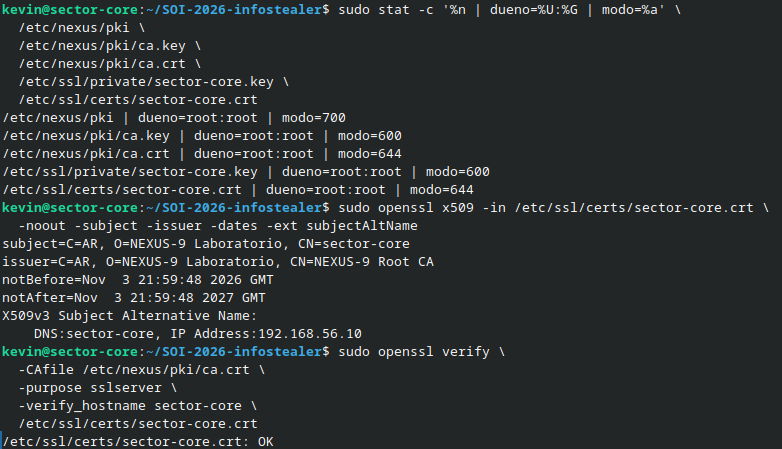
\includegraphics[width=0.88\textwidth]{images/E1_I16_01_https_certificado.png}
    \caption{Verificación de permisos, extensiones SAN y validación de cadena con la CA raíz del laboratorio.}
    \label{fig:e1_certificado}
\end{figure}

En la Figura~\ref{fig:e1_puertos} se documentan las pruebas de acceso realizadas desde \texttt{field-terminal}: la petición HTTPS a \texttt{https://sector-core/health} retorna exitosamente (\texttt{código 0}) sin requerir banderas inseguras, el acceso por HTTP plano (puerto 80) responde con redirección \texttt{301 Moved Permanently}, y el intento de acceder directamente al puerto interno 8080 es descartado por el firewall, culminando en un timeout (\texttt{curl: 28}).

\begin{figure}[H]
    \centering
    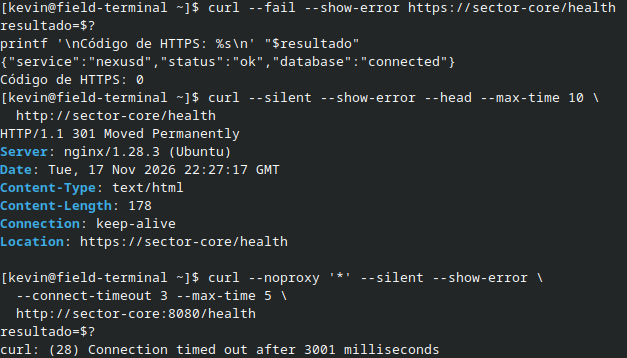
\includegraphics[width=0.88\textwidth]{images/E1_I16_02_puertos_8080_bloqueado.png}
    \caption{Petición HTTPS exitosa, redirección HTTP 301 y descarte de conexión directa al puerto 8080.}
    \label{fig:e1_puertos}
\end{figure}

% ==============================================================================
% SECCIÓN 2: ETAPA 02 — FIREWALL Y AISLAMIENTO CON SELINUX
% ==============================================================================
\section{Etapa 02 — Firewalling Perimetral y Aislamiento MAC con SELinux}

La seguridad en profundidad demanda que el acceso a los servicios esté controlado por capas independientes. Mientras Nginx gobierna la publicación a nivel de capa de aplicación, los firewalls del kernel (\texttt{netfilter}) determinan qué paquetes pueden alcanzar el host, y el sistema de Control de Acceso Obligatorio (\textbf{SELinux}) confina los privilegios de los procesos en ejecución.

\subsection{Políticas de Filtrado en \texttt{sector-core} y \texttt{field-terminal}}

Las reglas de filtrado se aplicaron mediante scripts declarativos e idempotentes, garantizando persistencia tras reinicios:

\begin{itemize}[leftmargin=*]
    \item \textbf{\texttt{sector-core} (\texttt{ufw}):} Política restrictiva: rechazo general entrante (\texttt{default deny incoming}) y permiso saliente. Reglas activas:
    \begin{itemize}
        \item \texttt{22/tcp ALLOW IN}: Acceso administrativo SSH y subsistema SFTP para transferencia de evidencias.
        \item \texttt{443/tcp ALLOW IN}: Tráfico HTTPS de la API pública atendido por Nginx.
        \item \texttt{80/tcp ALLOW IN}: Tráfico HTTP para permitir la respuesta de redirección 301.
        \item \texttt{8080/tcp DENY IN}: Bloqueo estricto del puerto interno de \texttt{nexusd}. Aunque el servicio escuche en loopback, esta regla previene cualquier exposición inadvertida ante errores de configuración.
    \end{itemize}
    \item \textbf{\texttt{field-terminal} (\texttt{firewalld}):} Configurado en la zona por defecto \texttt{public} aplicada a las interfaces de red. Dado que actúa como cliente del sector, se removieron los servicios prescindibles que ampliaban la superficie de ataque (\texttt{cockpit} en el puerto 9090 y \texttt{dhcpv6-client}), conservando únicamente el servicio \texttt{ssh} para propósitos de gestión.
\end{itemize}

\subsection{Confinamiento con SELinux en Rocky Linux}

En \texttt{field-terminal}, SELinux se mantuvo estrictamente en modo \textbf{Enforcing}. Para validar la capacidad de diagnóstico y resolución de eventos de denegación AVC (\textit{Access Vector Cache}), se analizó el caso donde \texttt{systemd} requería invocar scripts de operación del sector.

\begin{notabox}[Resolución de Denegación AVC Documentada]
    \textbf{Operación bloqueada:} \texttt{execute} sobre archivo de script.\\
    \textbf{Recurso y Contexto:} \texttt{/home/kevin/nexus-test.sh} etiquetado como \texttt{user\_home\_t} (\texttt{tclass=file}).\\
    \textbf{Sujeto:} Proceso gestor de servicios \texttt{systemd} en contexto \texttt{scontext=system\_u:system\_r:init\_t:s0}.\\
    \textbf{Diagnóstico:} La política de seguridad prohíbe que el dominio \texttt{init\_t} ejecute binarios o scripts ubicados en carpetas personales con contexto de usuario (\texttt{user\_home\_t}), fallando con \texttt{status=203/EXEC}.\\
    \textbf{Resolución Técnica:} Se reubicó el script en el directorio estándar del sistema \texttt{/usr/local/bin/}, asignándole el contexto legítimo de binarios del sistema \texttt{bin\_t} mediante \texttt{cp}. Se verificó con \texttt{ls -Z} y se reejecutó con \texttt{systemd-run}, culminando con \texttt{status=0/SUCCESS}. No se requirió desactivar SELinux ni relajar la política global.
\end{notabox}

\subsection{Respuestas a Preguntas de Investigación}

\begin{pregunta}{¿Qué diferencia hay entre rechazar (reject) y descartar (deny/drop) una conexión?}
    \textbf{Respuesta:} Con \textbf{REJECT}, el firewall intercepta el paquete y responde activamente al emisor con un mensaje ICMP (\textit{Destination Port Unreachable}) o un paquete TCP con el flag \texttt{RST} activo. El cliente detecta la denegación inmediatamente (\texttt{Connection refused}, código 7 en curl), lo que le permite saber que el host está vivo y el puerto cerrado.
    
    Con \textbf{DENY / DROP}, el firewall descarta silenciosamente el paquete sin enviar ninguna respuesta. El cliente debe esperar a que se agote su temporizador de conexión (\textit{timeout}, código 28 en curl). Esto añade latencia a posibles escaneos de puertos y evita confirmar la presencia del host o del firewall.
\end{pregunta}

\begin{pregunta}{¿Qué agrega SELinux por encima de los permisos tradicionales (DAC)?}
    \textbf{Respuesta:} El modelo tradicional DAC (\textit{Discretionary Access Control}) basa el acceso en el propietario y permisos del archivo (\texttt{rwxrwxrwx}). Si un atacante compromete un proceso corriendo como \texttt{root}, adquiere control total del sistema.
    
    SELinux implementa MAC (\textit{Mandatory Access Control}): el kernel asocia etiquetas de contexto (\texttt{usuario:rol:tipo:nivel}) a cada sujeto (proceso) y objeto (archivo, socket). Aunque un proceso corra como \texttt{root}, sólo puede interactuar con objetos explícitamente permitidos para su \textbf{tipo} en la matriz de políticas del kernel. Si un demonio es comprometido, queda atrapado dentro de su dominio sin poder acceder a archivos personales ni sockets no autorizados.
\end{pregunta}

\begin{pregunta}{Si \texttt{nexusd} ya escucha sólo en loopback, ¿para qué sirve además bloquear su puerto en el firewall?}
    \textbf{Respuesta:} Cumple con el principio de \textbf{defensa en profundidad}. Aunque hoy el software esté configurado para bindear a \texttt{127.0.0.1}, un error humano en un archivo de configuración, una actualización que cambie el valor por defecto a \texttt{0.0.0.0} o una falla de enlace podría exponer el puerto sin autenticación a la red. El firewall opera como un control perimetral independiente en la capa de red del kernel, impidiendo que el puerto sea alcanzado desde interfaces externas independientemente de cómo mute la aplicación interna.
\end{pregunta}

\begin{pregunta}{¿Qué diferencia hay entre activar un booleano de SELinux y cambiar el contexto de un archivo?}
    \textbf{Respuesta:} Un \textbf{booleano} de SELinux altera una regla lógica precompilada en la política del kernel (ej. permitir que Nginx se conecte a sockets de red con \texttt{httpd\_can\_network\_connect}); se utiliza cuando el comportamiento esperado ya está contemplado condicionalmente en la política estándar de la distribución. En contraste, \textbf{cambiar el contexto de un archivo} (\texttt{chcon} o \texttt{semanage fcontext}) redefine la etiqueta permanente del recurso en el sistema de archivos (ej. de \texttt{user\_home\_t} a \texttt{bin\_t}); se emplea cuando un archivo reside en una ruta personalizada y requiere ser clasificado para que los dominios autorizados puedan acceder a él según las reglas existentes.
\end{pregunta}

\subsection{Evidencia Experimental de la Etapa 02}

En la Figura~\ref{fig:e2_firewall} se exhibe el estado del firewall \texttt{ufw} en \texttt{sector-core} tras reiniciar el sistema operativo, confirmando la persistencia de las reglas de SSH, HTTPS, HTTP y el bloqueo de 8080 en IPv4 e IPv6, junto al estado activo de los daemons \texttt{nginx} y \texttt{nexus}.

\begin{figure}[H]
    \centering
    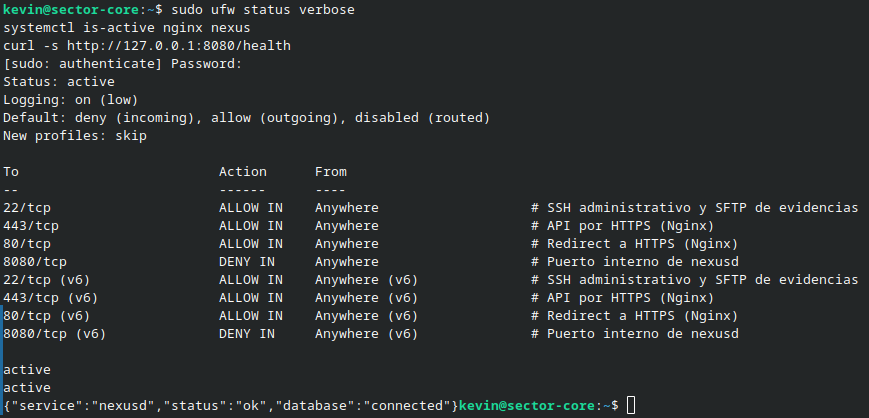
\includegraphics[width=0.88\textwidth]{images/E2_I26_01_firewall_tras_reinicio.png}
    \caption{Estado detallado de \texttt{ufw} en \texttt{sector-core} tras reinicio, validando persistencia y reglas.}
    \label{fig:e2_firewall}
\end{figure}

En la Figura~\ref{fig:e2_selinux} se demuestra la resolución técnica de la denegación de SELinux en \texttt{field-terminal}: reubicación a \texttt{/usr/local/bin}, constatación del contexto \texttt{unconfined\_u:object\_r:bin\_t:s0} y ejecución exitosa bajo \texttt{systemd-run} con resultado \texttt{status=0/SUCCESS}.

\begin{figure}[H]
    \centering
    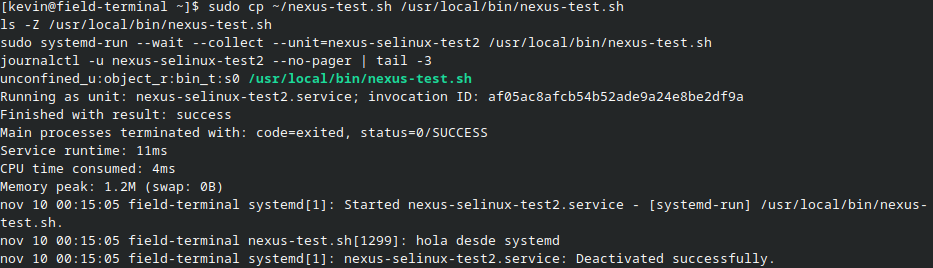
\includegraphics[width=0.88\textwidth]{images/E2_I24_02_selinux_denegacion_resuelta.png}
    \caption{Resolución de denegación de SELinux: asignación de contexto \texttt{bin\_t} y ejecución exitosa.}
    \label{fig:e2_selinux}
\end{figure}

En la Figura~\ref{fig:e2_firewalld} se documenta la comprobación de persistencia del firewall perimetral y el confinamiento de seguridad en \texttt{field-terminal} (Rocky Linux) tras reiniciar el sistema:
\begin{itemize}[leftmargin=*]
    \item \textbf{Zona activa y servicios:} El comando \texttt{sudo firewall-cmd --list-all} valida que la zona por defecto \texttt{public} gobierna activamente las interfaces \texttt{enp0s3} y \texttt{enp0s8}. En el listado de servicios figura de forma exclusiva \texttt{services: ssh}, certificando que los servicios prescindibles que ensanchaban la superficie de ataque (\texttt{cockpit} en el puerto 9090 y el cliente DHCPv6) fueron removidos permanentemente.
    \item \textbf{Confinamiento MAC persistente:} La consulta de \texttt{getenforce} ejecutada inmediatamente después corrobora que el kernel de Rocky Linux retoma la ejecución con SELinux en modo \textbf{Enforcing}, aplicando las restricciones de la política a los dominios confinados; este modo no demuestra por sí solo que todos los procesos tengan una política restrictiva.
\end{itemize}

\begin{figure}[H]
    \centering
    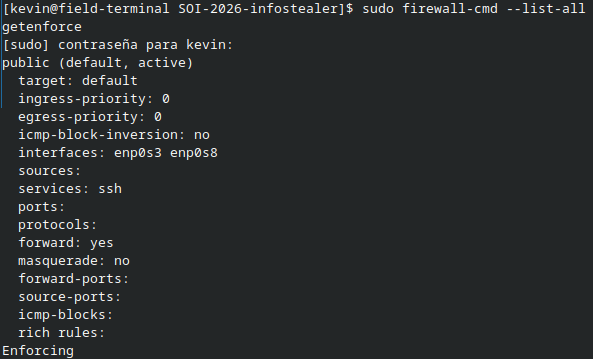
\includegraphics[width=0.88\textwidth]{images/E2_I26_02_firewalld_tras_reinicio.png}
    \caption{Estado persistente de \texttt{firewalld} en \texttt{field-terminal} tras reinicio: zona \texttt{public} con único servicio SSH y SELinux en modo \texttt{Enforcing}.}
    \label{fig:e2_firewalld}
\end{figure}

% ==============================================================================
% SECCIÓN 3: ETAPA 03 — EVIDENCIAS Y NOTIFICACIONES
% ==============================================================================
\section{Etapa 03 — Transferencia de Evidencias Segura y Notificaciones Internas}

La gestión forense y documental del sector requiere respaldar incidentes con archivos de evidencia fidedignos. Para no sobrecargar la API REST ni introducir vulnerabilidades de carga de archivos en el servicio HTTP, se implementó una estricta segregación de planos: \textbf{el archivo físico viaja por SFTP enjaulado y la API sólo almacena sus metadatos y sumas de control}.

\subsection{Confinamiento del Usuario de Carga (\texttt{nexus\_evidence})}

Se configuró una cuenta de servicio dedicada con mínimos privilegios:
\begin{itemize}[leftmargin=*]
    \item \textbf{Sin shell interactiva:} Shell asignada a \texttt{/usr/sbin/nologin}. Cualquier intento de conexión SSH interactiva es abortado de inmediato por el sistema operativo.
    \item \textbf{Enjaulamiento Chroot (\texttt{sshd\_config}):} Directivas configuradas en \texttt{/etc/ssh/sshd\_config}:
    \begin{terminalbox}{sshd_config fragment}
Match User nexus_evidence
    ChrootDirectory /srv/nexus-sftp
    ForceCommand internal-sftp -d /incoming -u 027
    AllowTcpForwarding no
    X11Forwarding no
    PasswordAuthentication no
    \end{terminalbox}
    Para satisfacer los estrictos requerimientos de seguridad de OpenSSH, el directorio raíz del chroot (\texttt{/srv/nexus-sftp}) es propiedad exclusiva de \texttt{root:root} con permisos \texttt{0755} (no escribible por el usuario, evitando fugas de la jaula). La recepción de archivos se realiza sobre el subdirectorio escribible \texttt{/srv/nexus-sftp/incoming}, el cual está enlazado mediante un \textbf{montaje bind} (\textit{bind mount}) al directorio de almacenamiento de evidencias (\path{/var/lib/nexus/evidence/incoming}), asignado a \texttt{nexus\_evidence:nexus} con permisos \texttt{2750}, con setgid para heredar el grupo nexus, permitiendo que las cargas se depositen directamente en la ruta de trabajo sin comprometer la seguridad del chroot.
\end{itemize}

\subsection{Flujo Transaccional del Script \texttt{upload-evidence.sh}}

La operación completa se orquesta desde \texttt{field-terminal} mediante el script \texttt{upload-evidence.sh}:
\begin{enumerate}[leftmargin=*]
    \item \textbf{Validación previa:} Comprueba la existencia y legibilidad del archivo local y los argumentos requeridos.
    \item \textbf{Cálculo de huella SHA-256:} Se computa el checksum criptográfico del archivo en el nodo de origen antes de la transmisión.
    \item \textbf{Transferencia SFTP segura:} Utilizando la llave SSH dedicada, se transmite el binario hacia \texttt{incoming/} en \texttt{sector-core}.
    \item \textbf{Asociación y validación por API:} El script invoca el endpoint de registro de evidencia. El backend en C recalcula el checksum sobre el archivo recibido en disco y valida su identidad. Si coinciden, los metadatos quedan asociados al incidente en SQLite y se emite un evento transaccional en la tabla de auditoría.
    \item \textbf{Manejo de errores y limpieza con \texttt{trap}:} Rutinas de captura de señales (\texttt{trap}) garantizan la eliminación de buffers temporales ante cualquier fallo.
\end{enumerate}

\subsection{Servicio de Notificaciones Operativas con Postfix}

Se configuró un agente de transporte de correo (\textbf{Postfix}) configurado estrictamente para \textbf{entrega local} en \texttt{sector-core}. Cuando \texttt{nexusd} registra un incidente con nivel de severidad \texttt{critical}, el módulo de notificaciones invoca el mecanismo local de envío para una alerta dirigida al buzón operativo local: \texttt{nexus-ops@sector-core}. La aceptación del envío se registra en el journal y la auditoría; la entrega efectiva al buzón se comprobó por separado en el ensayo.

\subsection{Respuestas a Preguntas de Investigación}

\begin{pregunta}{¿Qué condiciones debe cumplir un directorio para alojar un Chroot en OpenSSH?}
    \textbf{Respuesta:} El daemon \texttt{sshd} impone que cada componente del camino hacia el \texttt{ChrootDirectory} debe pertenecer a \textbf{\texttt{root}} y no puede tener permisos de escritura para el grupo ni para otros (\texttt{chmod go-w}). Si el usuario enjaulado tuviese permisos de escritura sobre la raíz del chroot, podría crear enlaces duros, manipular binarios o explotar vulnerabilidades locales para escapar del confinamiento de la jaula. Por tal motivo, los datos escribibles siempre se ubican en un subdirectorio interno (\texttt{incoming/}).
\end{pregunta}

\begin{pregunta}{¿Por qué un usuario de servicio no debería poder iniciar sesión normalmente?}
    \textbf{Respuesta:} Para reducir drásticamente la superficie de ataque del sistema (principio de mínimo privilegio). Un usuario de servicio como \texttt{nexus\_evidence} solo existe para ejecutar una tarea delimitada (recibir archivos por SFTP). Si dispusiera de una shell interactiva como \texttt{/bin/bash}, un atacante que comprometa su clave SSH obtendría una sesión de comandos en el servidor, pudiendo explorar procesos, inspeccionar variables de entorno y buscar vías de escalada de privilegios locales. Al asignarle \texttt{/usr/sbin/nologin} y forzar \texttt{internal-sftp}, se anula toda posibilidad de interacción en consola.
\end{pregunta}

\begin{pregunta}{¿Para qué sirve el checksum SHA-256 si el archivo ya llegó por SFTP?}
    \textbf{Respuesta:} Aunque SSH/SFTP garantiza la integridad de los paquetes durante la transmisión sobre el socket (mediante códigos MAC del canal cifrado), el checksum SHA-256 almacenado en la base de datos proporciona \textbf{no repudio y preservación de integridad en reposo a largo plazo}. Permite certificar que el archivo almacenado en disco meses después no ha sido alterado, corrompido por fallas de sectores de almacenamiento o modificado por un actor no autorizado dentro del servidor.
\end{pregunta}

\begin{pregunta}{¿Qué debería pasar si el checksum calculado no coincide con el registrado?}
    \textbf{Respuesta:} La API debe rechazar la asociación inmediatamente con un código de error semántico (HTTP \texttt{400 Bad Request} o \texttt{422 Unprocessable Entity}), eliminar el archivo potencialmente corrupto o incompleto de la zona de trabajo, y registrar un evento de falla en la tabla de auditoría. El incidente no debe vincular evidencia corrupta bajo ninguna circunstancia.
\end{pregunta}

\subsection{Evidencia Experimental de la Etapa 03}

En la Figura~\ref{fig:e3_evidencia} se documenta la ejecución exitosa de \texttt{upload-evidence.sh} desde \texttt{field-terminal}, transfiriendo el binario \texttt{evi-e310.bin} y registrándolo para el incidente \#1 con su correspondiente SHA-256 calculado (\texttt{código 0}).

\begin{figure}[H]
    \centering
    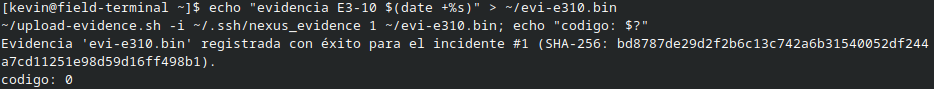
\includegraphics[width=0.88\textwidth]{images/E3_I36_01_carga_registro_evidencia.png}
    \caption{Transferencia SFTP de evidencia y confirmación de registro criptográfico SHA-256 vía API.}
    \label{fig:e3_evidencia}
\end{figure}

En la Figura~\ref{fig:e3_notificacion} se verifica la creación de un incidente crítico, evidenciando en el journal de \texttt{nexusd} el despacho de la notificación (\texttt{entrega=OK}) y el evento en auditoría (\texttt{NOTIFY\_INCIDENT}), junto a la lectura del correo electrónico en el buzón local \texttt{/var/mail/nexus-ops}.

\begin{figure}[H]
    \centering
    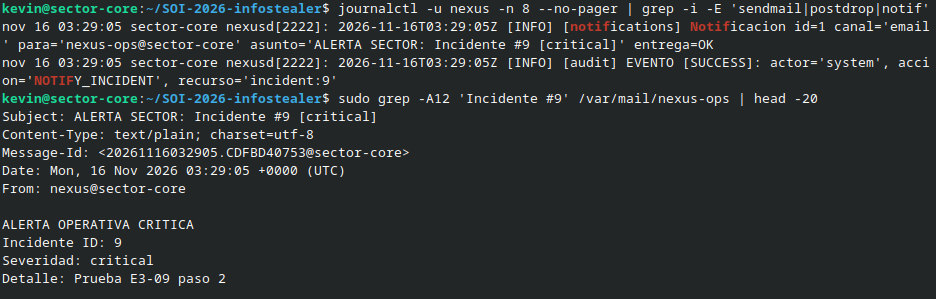
\includegraphics[width=0.88\textwidth]{images/E3_I35_02_notificacion_critica.png}
    \caption{Notificación local automática ante incidente crítico y recepción en \texttt{/var/mail/nexus-ops}.}
    \label{fig:e3_notificacion}
\end{figure}

En la Figura~\ref{fig:e3_ssh_rechazo} y Figura~\ref{fig:e3_sftp_chroot} se documentan las pruebas de seguridad negativas aplicadas a la cuenta \texttt{nexus\_evidence} desde \texttt{field-terminal}:
\begin{itemize}[leftmargin=*]
    \item \textbf{Rechazo de Shell y Comandos Remotos (Figura~\ref{fig:e3_ssh_rechazo}):} El intento de apertura de sesión interactiva SSH (\texttt{ssh -i} \path{~/.ssh/nexus_evidence} \nolinkurl{nexus_evidence@sector-core}) o la ejecución remota de binarios (\texttt{ssh} con el comando remoto \texttt{id}) es abortado inmediatamente por el subsistema OpenSSH emitiendo el mensaje \texttt{"This service allows sftp connections only."} y cerrando la conexión.
    \item \textbf{Aislamiento Chroot (Figura~\ref{fig:e3_sftp_chroot}):} Al iniciar sesión SFTP legítima, el entorno queda confinado en su raíz virtual: \texttt{ls /} exhibe de forma exclusiva la carpeta de subida autorizada (\texttt{/incoming}), intentos de navegación transversal (\texttt{cd /etc}) devuelven \texttt{No such file or directory}, y cualquier tentativa de escribir fuera de la jaula (\texttt{put ... /hostname}) es rechazada con \texttt{Permission denied}.
\end{itemize}

\begin{figure}[H]
    \centering
    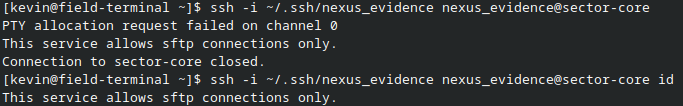
\includegraphics[width=0.92\textwidth]{images/E3_I31_01_ssh_no_shell.png}
    \caption{Pruebas negativas de acceso: rechazo taxativo de shell interactiva y comandos remotos en OpenSSH.}
    \label{fig:e3_ssh_rechazo}
\end{figure}

\begin{figure}[H]
    \centering
    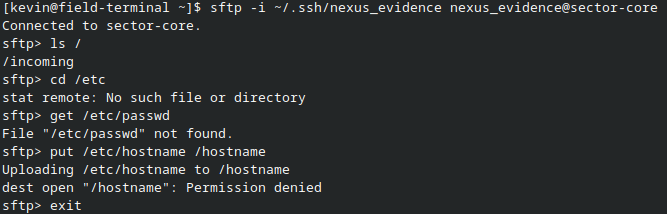
\includegraphics[width=0.92\textwidth]{images/E3_I31_02_sftp_chroot_incoming.png}
    \caption{Confinamiento Chroot de SFTP: visibilidad restringida y denegación de escritura fuera de \texttt{/incoming}.}
    \label{fig:e3_sftp_chroot}
\end{figure}

% ==============================================================================
% SECCIÓN 4: ETAPA 04 — RESILIENCIA, GOBERNANZA DE RECURSOS Y LOGS
% ==============================================================================
\section{Etapa 04 — Resiliencia, Gobernanza de Recursos en Systemd y Rotación de Logs}

Para asegurar la continuidad operativa y evitar que comportamientos anómalos degraden la máquina anfitriona, el servicio \texttt{nexus.service} fue endurecido mediante directivas de supervisión, límites de cgroups y confinamiento de sistema de archivos.

\subsection{Endurecimiento de \texttt{nexus.service}}

\begin{table}[H]
    \centering
    \footnotesize
    \caption{Directivas de control de recursos y resiliencia implementadas en \texttt{nexus.service}.}
    \label{tab:systemd_resiliencia}
    \begin{tabularx}{\textwidth}{llX}
        \toprule
        \rowcolor{tableheader}
        \textbf{Categoría} & \textbf{Directiva} & \textbf{Fundamentación Técnica y Comportamiento} \\
        \midrule
        \textbf{Reinicio Automático} & \texttt{Restart=on-failure} & Reinicia el proceso si termina de forma anormal o por señal no controlada. \\
        & \texttt{RestartSec=2} & Lapso de gracia antes del reintento; minimiza el impacto de reinicios en ráfaga. \\
        & \texttt{StartLimitBurst=5} & Cancela reintentos si ocurren más de 5 caídas en 60 segundos, evitando bucles infinitos. \\
        \rowcolor{rowalt}
        \textbf{Límites de Cgroup} & \texttt{MemoryHigh=64M} & Umbral de advertencia: el kernel frena la asignación y reclama memoria caché. \\
        & \texttt{MemoryMax=96M} & Límite absoluto (OOM killer de cgroup termina el proceso ante fugas descontroladas). \\
        & \texttt{CPUQuota=50\%} & Concede como máximo medio núcleo de procesamiento, preservando CPU para SSH y Nginx. \\
        & \texttt{TasksMax=64} & Limita la creación de hilos y subprocesos para impedir ataques tipo \textit{fork bomb}. \\
        \rowcolor{rowalt}
        \textbf{Aislamiento de FS} & \texttt{ProtectSystem=strict} & Todo el árbol raíz (\texttt{/}, \texttt{/usr}, \texttt{/etc}) se monta en modo de sólo lectura. \\
        & \texttt{ProtectHome=true} & Aísla completamente los directorios de usuarios (\texttt{/home}, \texttt{/root}). \\
        & \texttt{PrivateTmp=true} & Espacio de nombres de \texttt{/tmp} exclusivo y desvinculado del sistema. \\
        & \texttt{ReadWritePaths} & Acceso de escritura exclusivo sobre \texttt{/var/lib/nexus} (necesario para WAL SQLite). \\
        \bottomrule
    \end{tabularx}
\end{table}

\subsection{Estrategia de Rotación de Logs (\texttt{logrotate})}

El proceso \texttt{nexusd} emite trazas duales: a \texttt{stderr} (capturadas por \texttt{systemd-journald}) y al archivo dedicado \texttt{/var/log/nexus/nexusd.log}. Para evitar el llenado del disco, se configuró \texttt{/etc/logrotate.d/nexus}:
\begin{itemize}[leftmargin=*]
    \item \textbf{Frecuencia y retención:} Rotación diaria (\texttt{daily}), conservando 7 generaciones (\texttt{rotate 7}).
    \item \textbf{Compresión inteligente:} \texttt{compress} y \texttt{delaycompress} (mantiene la copia más reciente sin comprimir para lecturas rápidas de incidentes recientes).
    \item \textbf{Señalización atómica con SIGHUP:} Tras rotar el archivo, la directiva \texttt{postrotate} invoca \texttt{systemctl reload nexus}. El demonio intercepta la señal POSIX \texttt{SIGHUP}, cierra su descriptor de archivo antiguo y reabre el nuevo sin reiniciar el proceso ni perder trazas intermedias.
\end{itemize}

\subsection{Evidencia Experimental de la Etapa 04}

En la Figura~\ref{fig:e4_recuperacion} se demuestra la recuperación automática del servicio: se eliminó abruptamente el proceso mediante \texttt{kill -9}, y \texttt{systemd} lo detectó de inmediato, levantando una nueva instancia con un nuevo PID y reflejando \texttt{NRestarts=1}.

\begin{figure}[H]
    \centering
    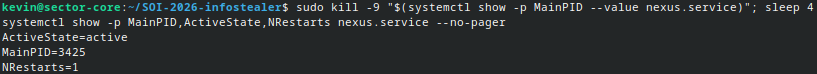
\includegraphics[width=0.88\textwidth]{images/E4_I42_01_recuperacion_automatica.png}
    \caption{Prueba de resiliencia ante caída forzada (\texttt{kill -9}) y recuperación automática por systemd.}
    \label{fig:e4_recuperacion}
\end{figure}

En la Figura~\ref{fig:e4_logrotate} se exhibe la ejecución de rotación forzada con \texttt{logrotate -f}, evidenciando la generación de \texttt{nexusd.log.1}, el nuevo archivo \texttt{nexusd.log} reabierto con permisos \texttt{nexus:nexus} y el servicio activo.

\begin{figure}[H]
    \centering
    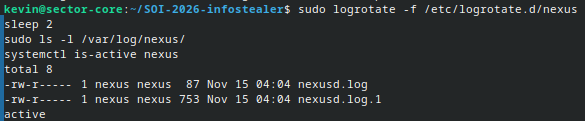
\includegraphics[width=0.88\textwidth]{images/E4_I45_02_rotacion_logs.png}
    \caption{Rotación efectiva de logs en \texttt{/var/log/nexus/} y preservación del servicio en ejecución.}
    \label{fig:e4_logrotate}
\end{figure}

En la Figura~\ref{fig:e4_limites_mem} y Figura~\ref{fig:e4_limites_cpu} se constata la inspección en vivo de los controladores de recursos cgroups v2 aplicados sobre \texttt{nexus.service} mediante \texttt{systemctl show}:
\begin{itemize}[leftmargin=*]
    \item \textbf{Límites de Memoria (Figura~\ref{fig:e4_limites_mem}):} Se corrobora \texttt{MemoryHigh=67108864} (64 MiB como umbral de contención) y \texttt{MemoryMax=100663296} (96 MiB como techo absoluto antes de activación del OOM Killer defensivo).
    \item \textbf{Límites de CPU y Tareas (Figura~\ref{fig:e4_limites_cpu}):} Se verifica \texttt{CPUQuotaPerSecUSec=500ms} (equivalente a una cuota estricta del 50\% de un núcleo de procesamiento) y \texttt{TasksMax=64} (techo máximo de hilos/procesos concurrentes para prevenir bifurcaciones incontroladas).
\end{itemize}

\begin{figure}[H]
    \centering
    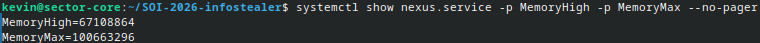
\includegraphics[width=0.88\textwidth]{images/E4_I38_01_limites_memoria.png}
    \caption{Gobernanza de memoria en Systemd: inspección de \texttt{MemoryHigh} (64 MB) y \texttt{MemoryMax} (96 MB).}
    \label{fig:e4_limites_mem}
\end{figure}

\begin{figure}[H]
    \centering
    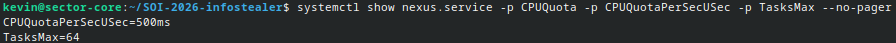
\includegraphics[width=0.88\textwidth]{images/E4_I39_02_limites_cpu_tareas.png}
    \caption{Límites de procesamiento en Systemd: cuota de CPU (\texttt{500ms}) y límite de concurrencia (\texttt{TasksMax=64}).}
    \label{fig:e4_limites_cpu}
\end{figure}

% ==============================================================================
% SECCIÓN 5: ETAPA 05 — BACKUPS Y RESTAURACIÓN
% ==============================================================================
\section{Etapa 05 — Continuidad Operativa: Estrategia de Backups y Restauración}

La información operativa (incidentes, unidades, evidencias y auditoría) constituye el activo irremplazable del sector. Se implementó una política integral de copias de seguridad atómicas, verificación criptográfica independiente y procedimientos probados de recuperación ante desastres.

\subsection{Generación de Copias Consistentes (\texttt{backup.sh})}

El script \texttt{scripts/backup.sh} genera una copia estructurada en \path{/var/backups/nexus/nexus-backup-AAAAMMDD-HHMMSS/}:
\begin{itemize}[leftmargin=*]
    \item \textbf{Consistencia de SQLite:} Se utiliza el comando de respaldo en caliente de la base (\texttt{sqlite3 .backup}) o copia transaccional sin transacciones incompletas, evitando corrupciones derivadas de los archivos auxiliares de WAL (\texttt{.db-wal} y \texttt{.db-shm}).
    \item \textbf{Copia de configuración y evidencias:} Se respaldan \texttt{nexus.conf} y el árbol íntegro de \texttt{evidence/}.
    \item \textbf{Manifiesto criptográfico (\texttt{manifest.sha256} y \texttt{manifest.info}):} Registra marcas temporales, versión y la suma de control SHA-256 de cada archivo individual incluido en la copia.
    \item \textbf{Verificación en frío (\texttt{--verify}):} Permite comprobar la integridad física y matemática de la copia en disco sin necesidad de restaurarla en la base de datos de producción.
\end{itemize}

\subsection{Automatización con Temporizadores Systemd y Retención}

Se crearon las unidades \texttt{nexus-backup.service} (\texttt{Type=oneshot}) y \nolinkurl{nexus-backup.timer}:
\begin{itemize}[leftmargin=*]
    \item \textbf{Temporización estricta:} \texttt{OnCalendar=*-*-* 03:00:00 UTC}, programando la ejecución en horas de baja actividad.
    \item \textbf{Persistencia (\texttt{Persistent=true}):} Si la máquina permaneció apagada durante el horario fijado, systemd dispara el respaldo inmediatamente al siguiente encendido.
    \item \textbf{Retención automática:} Política de 7 copias diarias (\texttt{--retention-days 7} y \texttt{--max-backups 7}). Las copias más antiguas son depuradas automáticamente de forma ordenada.
\end{itemize}

\subsection{Procedimiento de Restauración Verificada (\texttt{restore.sh})}

El script \texttt{scripts/restore.sh} implementa una secuencia estrictamente defensiva:
\begin{enumerate}[leftmargin=*]
    \item \textbf{Validación previa del manifiesto:} Comprueba que los hashes SHA-256 de todos los archivos del backup coincidan. Si un solo archivo fue manipulado o corrompido, \textbf{la restauración se aborta inmediatamente con código 2 sin tocar el estado actual}.
    \item \textbf{Detención del servicio y Snapshot preventivo:} Se detiene \texttt{nexus.service} y se genera una copia de seguridad del estado actual previo a la sobreescritura (\texttt{pre-restore-*}).
    \item \textbf{Restauración atómica y reactivación:} Se reemplazan la base SQLite y los archivos de evidencias preservando permisos y montajes, se eliminan restos de WAL desactualizados y se reanuda el daemon.
\end{enumerate}

\subsection{Respuestas a Preguntas de Investigación}

\begin{pregunta}{¿Por qué copiar el archivo SQLite con cp no garantiza una copia consistente?}
    \textbf{Respuesta:} SQLite en modo WAL mantiene páginas en memoria intermedia y en el archivo auxiliar \texttt{.db-wal} que se sincronizan asíncronamente con el archivo principal \texttt{.db}. Si se utiliza un comando plano como \texttt{cp} mientras la aplicación escribe, \texttt{cp} lee bloques de disco en momentos temporales ligeramente distintos, copiando un archivo \texttt{.db} a medio actualizar sin su correspondiente WAL sincronizado. El archivo resultante puede quedar corrupto e ilegible. La API de backup de SQLite (\texttt{.backup}) interactúa con el motor para adquirir locks compartidos ordenados y generar una instantánea físicamente consistente.
\end{pregunta}

\begin{pregunta}{Un backup que nunca se restauró, ¿es realmente un backup?}
    \textbf{Respuesta:} No. Es únicamente un archivo en disco con potencial de servir como backup. Hasta que no se ejecuta un procedimiento de restauración en un entorno real y se verifica la validez semántica de los datos recuperados, no existe garantía alguna de que la copia no contenga fallas lógicas, discrepancias de permisos o corrupción oculta. La única medida real de éxito de un sistema de copias es su capacidad comprobada de restauración (\textit{RTO} y \textit{RPO}).
\end{pregunta}

\begin{pregunta}{¿Qué diferencia hay entre un timer de systemd y una entrada de cron?}
    \textbf{Respuesta:} Un temporizador de systemd gestiona la ejecución mediante una unidad independiente de tipo \texttt{.timer} que activa una unidad \texttt{.service}. Esto aporta ventajas sustanciales sobre cron: supervisión nativa en journald con registros unificados, control estricto de recursos y aislamiento mediante cgroups, dependencias declarativas explícitas con otros servicios del sistema, y la directiva \texttt{Persistent=true} para gestionar ejecuciones perdidas.
\end{pregunta}

\begin{pregunta}{¿Qué ocurre con un timer si la máquina estaba apagada a la hora programada?}
    \textbf{Respuesta:} Si la directiva \texttt{Persistent=true} está configurada en la sección \texttt{[Timer]}, systemd guarda en disco una marca temporal de la última ejecución en \texttt{/var/lib/systemd/timers/}. Al encender la máquina tras haber estado apagada durante la ventana programada, systemd detecta el evento perdido y dispara inmediatamente el servicio asociado. En cron tradicional, la tarea simplemente se omite hasta el siguiente ciclo a menos que se configure una herramienta adicional como anacron.
\end{pregunta}

\subsection{Evidencia Experimental de la Etapa 05}

En la Figura~\ref{fig:e5_manifest} se visualiza la inspección del archivo \texttt{manifest.info} y la validación de integridad criptográfica exitosa ejecutando \texttt{backup.sh --verify} (\texttt{código 0}).

\begin{figure}[H]
    \centering
    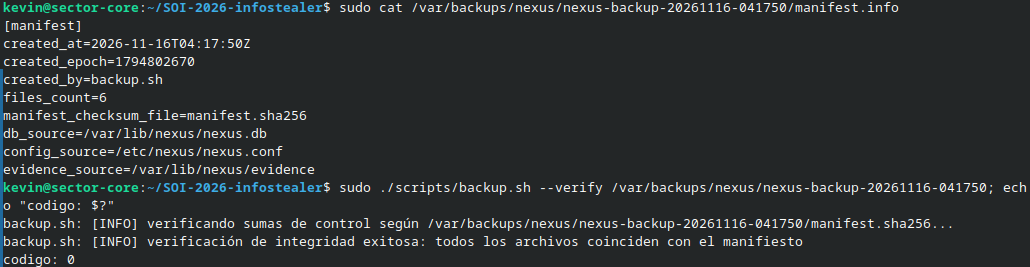
\includegraphics[width=0.88\textwidth]{images/E5_I49_01_backup_verificado.png}
    \caption{Inspección de metadatos en manifiesto y verificación de integridad de backup en frío.}
    \label{fig:e5_manifest}
\end{figure}

En la Figura~\ref{fig:e5_corrupto} se documenta el comportamiento defensivo ante fallos: la ejecución del test de regresión \texttt{test-restore-corrupt.sh} demuestra que ante la manipulación deliberada de la base o de evidencias, \texttt{restore.sh} detecta la discrepancia de hash, rechaza la operación con \texttt{código 2} y preserva los datos preexistentes intactos.

\begin{figure}[H]
    \centering
    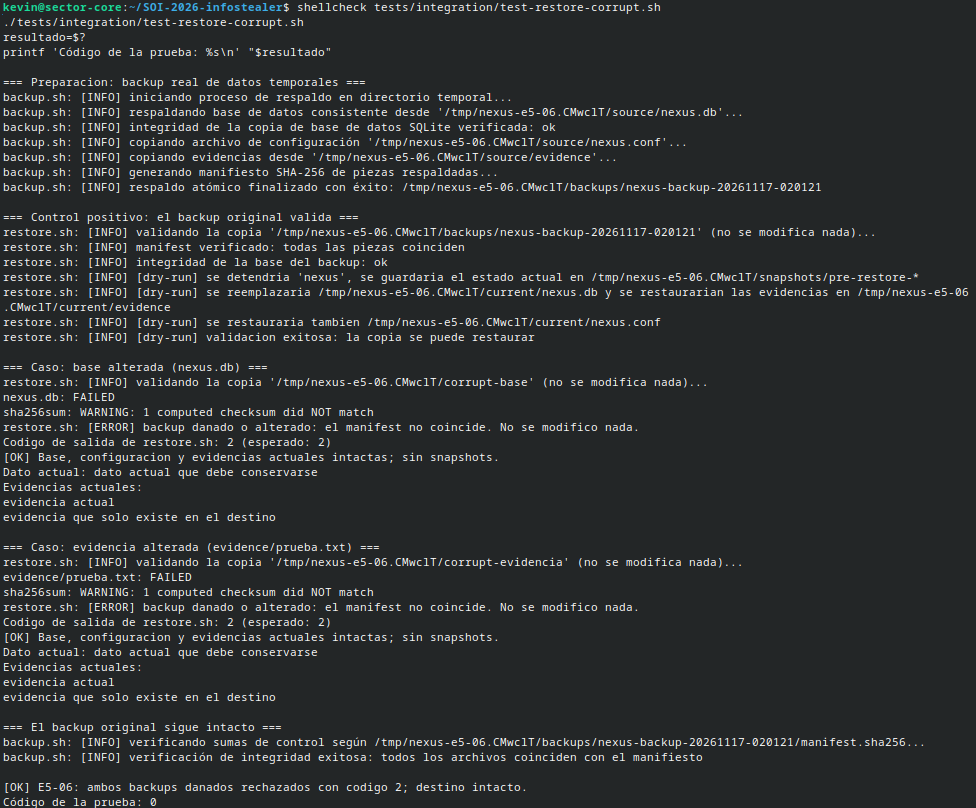
\includegraphics[width=0.88\textwidth]{images/E5_I52_02_backup_corrupto_rechazado.png}
    \caption{Rechazo preventivo garantizado de copias de seguridad corruptas o inconsistentes.}
    \label{fig:e5_corrupto}
\end{figure}

En la Figura~\ref{fig:e5_restauracion} se documenta la prueba de recuperación ante una pérdida real: se eliminaron físicamente la base \texttt{nexus.db} y los archivos de evidencia, se ejecutó \texttt{restore.sh} y se constató la restitución completa del sistema con código de salida 0.

\begin{figure}[H]
    \centering
    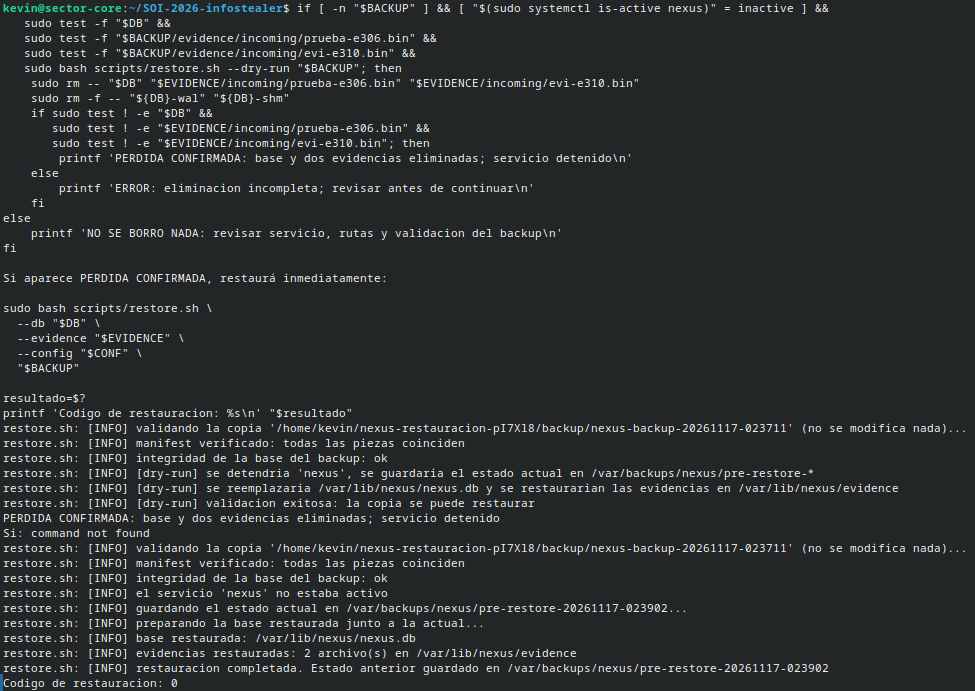
\includegraphics[width=0.88\textwidth]{images/E5_I56_03_restauracion_real.png}
    \caption{Simulación de pérdida real provocada y restauración íntegra de base de datos y evidencias.}
    \label{fig:e5_restauracion}
\end{figure}

En la Figura~\ref{fig:e5_timer} se corrobora el aprovisionamiento y funcionamiento del temporizador automatizado \nolinkurl{nexus-backup.timer}:
\begin{itemize}[leftmargin=*]
    \item \textbf{Programación temporal y estado activo:} La unidad se encuentra en estado \texttt{enabled} y \texttt{active}. El comando \texttt{systemctl list-timers} confirma la correspondencia con \texttt{nexus-backup.service}, reportando la próxima ejecución programada a las 03:00:00 UTC con el retraso aleatorio configurado.
    \item \textbf{Directivas de resiliencia:} La inspección mediante \texttt{systemctl show} certifica la persistencia operativa ante eventuales apagados de la máquina virtual (\texttt{Persistent=yes}) y la aplicación del mecanismo de dispersión de carga (\texttt{RandomizedDelayUSec=15min}).
\end{itemize}

\begin{figure}[H]
    \centering
    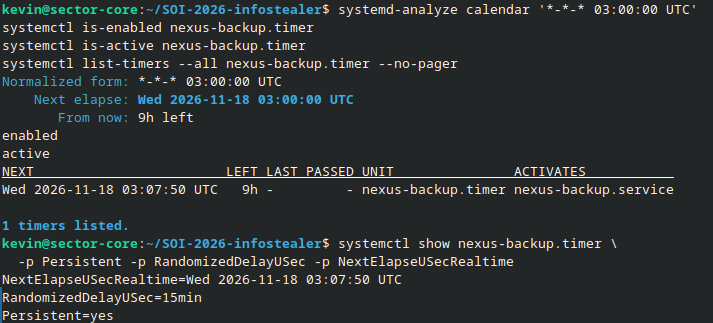
\includegraphics[width=0.92\textwidth]{images/E5_I54_01_backup_timer.png}
    \caption{Estado activo y programación del temporizador \nolinkurl{nexus-backup.timer} con persistencia y retraso aleatorio.}
    \label{fig:e5_timer}
\end{figure}

% ==============================================================================
% SECCIÓN 6: ETAPA 06 — OBSERVABILIDAD Y DIAGNÓSTICO
% ==============================================================================
\section{Etapa 06 — Observabilidad: Monitor de Salud y Diagnóstico Sanitizado}

Para responder con certeza a los estados operativos del sistema (*"¿está todo bien?"* y, ante anomalías, *"¿qué falló?"*), se diseñaron dos herramientas modulares de observabilidad con contratos rigurosos de ejecución.

\subsection{Monitor de Salud Multipunto (\texttt{health-check.sh})}

El script \texttt{scripts/health-check.sh} evalúa de punta a punta la pila de servicios:
\begin{itemize}[leftmargin=*]
    \item \textbf{Estado de servicios Systemd:} Confirma que las unidades \texttt{nexus.service} y \texttt{nginx.service} estén en estado \texttt{active}.
    \item \textbf{Conectividad HTTPS real:} Realiza una petición completa sobre TLS validando la CA del laboratorio contra \texttt{https://sector-core/health}.
    \item \textbf{Persistencia y base SQLite:} Verifica la existencia física y legibilidad de \texttt{nexus.db}.
    \item \textbf{Capacidad de almacenamiento:} Comprueba que la partición \texttt{/var/lib/nexus} no supere el umbral crítico de saturación de disco.
    \item \textbf{Frescura de copias de seguridad:} Valida que la última copia generada por \texttt{nexus-backup.service} sea reciente y tenga integridad válida.
    \item \textbf{Códigos de salida semánticos:} Retorna \texttt{0} para un sistema íntegramente sano, y códigos mayores a 0 ante estados degradados o caídos.
\end{itemize}

\subsection{Recolector de Diagnósticos Forenses (\texttt{collect-diagnostics.sh})}

Cuando ocurre una contingencia, el estado volátil cambia rápidamente. El recolector empaqueta una fotografía estructurada del sistema. El archivo se identifica por fecha UTC: \nolinkurl{nexus-diagnostics-AAAAMMDD-HHMMSS.tar.gz}. Incluye:
\begin{itemize}[leftmargin=*]
    \item \textbf{Secciones estructuradas:} Recopila información del sistema operativo (\texttt{01-system-info}), estado de unidades systemd (\texttt{02-services}), procesos activos (\texttt{03-processes}, registrando estado y porcentaje promedio de CPU reportado por \texttt{ps}), interfaces y tablas de red (\texttt{04-network}), reglas de firewall (\texttt{05-firewall}), estado de SELinux (\texttt{06-selinux}, capturando denegaciones AVC dentro de la ventana reciente de auditoría), almacenamiento (\texttt{07-storage}), resultado del health-check y últimos registros de log.
    \item \textbf{Sanitización de secretos y seguridad:} Aplica un filtro de sanitización mediante expresiones regulares para detectar patrones conocidos de claves privadas (ej. \texttt{BEGIN RSA PRIVATE KEY}), contraseñas y tokens sensibles, reemplazando el contenido íntegro del archivo afectado por un aviso \texttt{[REDACTED]}; no se limita a sustituir las coincidencias aisladas. Si bien esta técnica mitiga la filtración involuntaria de credenciales estándar antes de compartir diagnósticos externamente, no ofrece una garantía matemática absoluta frente a formatos no convencionales o secretos embebidos en texto plano arbitrario, requiriendo verificación humana prudente. El archivo final se genera con permisos restrictivos \texttt{0600}.
\end{itemize}

\subsection{Respuestas a Preguntas de Investigación}

\begin{pregunta}{¿Qué diferencia hay entre "el proceso está corriendo" y "el servicio está sano"?}
    \textbf{Respuesta:} Que un proceso exista en la tabla de procesos del kernel (con PID asignado y estado \texttt{R} o \texttt{S}) únicamente indica que no ha terminado. Sin embargo, el servicio puede estar completamente inutilizable: atrapado en un interbloqueo (\textit{deadlock}), con la base de datos desconectada o bloqueada, con sus descriptores de socket agotados o sin atender conexiones HTTP entrantes. "Estar sano" implica que el servicio es capaz de responder satisfactoriamente a las peticiones reales del cliente respetando su contrato de interfaz (semántica de *readiness*).
\end{pregunta}

\begin{pregunta}{¿Qué debería devolver el health check si la aplicación responde pero el disco está casi lleno?}
    \textbf{Respuesta:} Debe devolver un código de estado intermedio de advertencia o sistema degradado (código no nulo, ej. \texttt{código 1} o \texttt{código 2}). Aunque la API responda en memoria en ese instante, el sistema es incapaz de persistir nuevos incidentes, registrar auditorías o recibir evidencias por SFTP. Alertar proactivamente antes de que ocurra el fallo catastrófico por falta de espacio es el propósito fundamental de un monitor de salud.
\end{pregunta}

\begin{pregunta}{¿Cuántos estados distintos necesita informar y cómo se representan en un código de salida?}
    \textbf{Respuesta:} Requiere informar al menos tres estados claramente discernibles: \textbf{0 (Sano / OK)} si todos los componentes operan nominalmente; \textbf{1 (Degradado / Advertencia)} si el servicio responde pero existen umbrales de riesgo (ej. espacio en disco bajo o backup desactualizado); y \textbf{2 o superior (Crítico / Fallo)} si un daemon vital está caído, el puerto cerrado o la base inaccesible. En sistemas Unix, reflejar estos estados en el código de salida (\textit{exit status}) permite a scripts de orquestación (como \texttt{deploy.sh}) tomar decisiones automatizadas inmediatas sin necesidad de parsear texto.
\end{pregunta}

\begin{pregunta}{¿Qué información no debería incluirse nunca en un paquete de diagnóstico?}
    \textbf{Respuesta:} Claves privadas criptográficas (claves privadas SSH de usuarios o de la CA, clave privada TLS del servidor web), credenciales o contraseñas en texto plano, tokens de autorización activos y datos personales sensibles regulados. La inclusión involuntaria de claves privadas comprometería permanentemente la identidad y el cifrado de la infraestructura si el archivo es transferido a terceros para depuración.
\end{pregunta}

\begin{pregunta}{¿Para qué sirve recolectar el estado del sistema en el momento de la falla en lugar de después?}
    \textbf{Respuesta:} Porque la información forense más crítica es altamente volátil: tablas de conexiones TCP activas (\texttt{ss}), procesos en estado zombie o bloqueados en D (\textit{uninterruptible sleep}), buffers de memoria del kernel, denegaciones recientes en auditd y descriptores abiertos. Si se espera a reiniciar el servicio o la máquina, o si se permite que pasen minutos, el sistema operativo limpia esos recursos volátiles y la causa raíz (\textit{root cause}) del problema se vuelve irrecuperable.
\end{pregunta}

\subsection{Evidencia Experimental de la Etapa 06}

En la Figura~\ref{fig:e6_health} se constata la ejecución del monitor de salud evaluando positivamente cada componente y reportando \texttt{Resultado: SANO (código 0)}.

\begin{figure}[H]
    \centering
    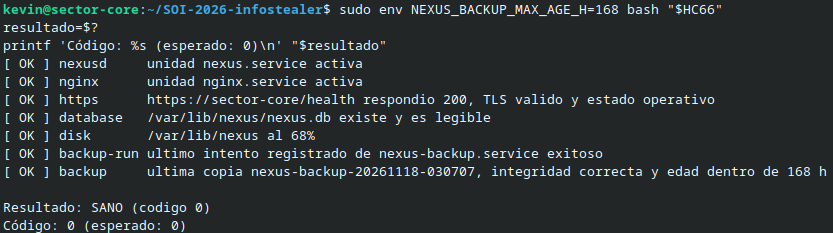
\includegraphics[width=0.88\textwidth]{images/E6_I62_01_health.png}
    \caption{Evaluación de salud integral con \texttt{health-check.sh} en estado plenamente operativo.}
    \label{fig:e6_health}
\end{figure}

En la Figura~\ref{fig:e6_diagnostics} se visualiza la generación del paquete de diagnósticos con marca de tiempo UTC, permisos \texttt{0600} y el desglose de sus componentes estructurados mediante \texttt{tar -tzf}.

\begin{figure}[H]
    \centering
    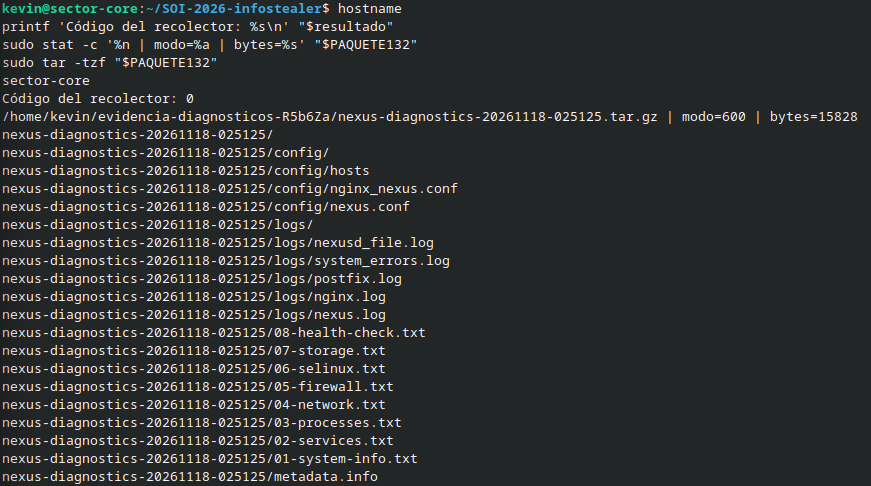
\includegraphics[width=0.88\textwidth]{images/E6_I63_02_paquete_diagnostico.png}
    \caption{Estructura del archivo de diagnóstico generado por \texttt{collect-diagnostics.sh}.}
    \label{fig:e6_diagnostics}
\end{figure}

% ==============================================================================
% SECCIÓN 7: ETAPA 07 — CLIENTE DEL OPERADOR EN C (nexusctl)
% ==============================================================================
\section{Etapa 07 — Cliente Nativo de Operador en C (\texttt{nexusctl})}

Para la operación profesional de campo en \texttt{field-terminal}, se reemplazó el cliente provisional en shell por una aplicación compilada nativa en lenguaje C (\textbf{\texttt{nexusctl}}), enlazada contra \textbf{\texttt{libcurl}} y construida con el mismo sistema de build de la plataforma.

\subsection{Arquitectura y Precedencia de Configuración}

Siguiendo las mejores prácticas de seguridad operativa, \textbf{ninguna dirección de servidor se encuentra codificada de forma rígida (\textit{hardcoded}) en el código fuente}. El cliente resuelve la URL destino mediante una cascada estricta:
\begin{enumerate}[leftmargin=*]
    \item Parámetro explícito en línea de comandos: \texttt{--server <URL>} o \texttt{-s <URL>}.
    \item Variable de entorno principal: \texttt{\$NEXUS\_API\_URL}.
    \item Variable de entorno heredada: \texttt{\$NEXUS\_URL}.
    \item Archivo de configuración local: Clave \texttt{server} en \texttt{/etc/nexus/nexusctl.conf}.
    \item Si ninguna está configurada: El programa aborta de inmediato con mensaje claro y \textbf{código de salida 1}.
\end{enumerate}

\subsection{Contrato de Códigos de Salida de \texttt{nexusctl}}

Para permitir su integración en scripts de orquestación, \texttt{nexusctl} distingue con precisión la causa de cualquier terminación:

\begin{table}[H]
    \centering
    \footnotesize
    \caption{Contrato de códigos de salida semánticos del cliente \texttt{nexusctl}.}
    \label{tab:nexusctl_exit_codes}
    \begin{tabularx}{\textwidth}{cclX}
        \toprule
        \rowcolor{tableheader}
        \textbf{Código} & \textbf{Macro en C} & \textbf{Condición} & \textbf{Criterio Semántico de Activación} \\
        \midrule
        \textbf{0} & \texttt{NEXUSCTL\_EXIT\_OK} & Éxito & Respuesta HTTP 2xx y procesamiento JSON conforme al contrato. \\
        \rowcolor{rowalt}
        \textbf{1} & \texttt{NEXUSCTL\_EXIT\_USAGE} & Error de Uso & Sintaxis errónea, argumentos faltantes o URL de servidor ausente. \\
        \textbf{2} & \texttt{NEXUSCTL\_EXIT\_API\_ERROR} & Error de API & La API respondió con código de error HTTP (4xx o 5xx). \\
        \rowcolor{rowalt}
        \textbf{3} & \texttt{NEXUSCTL\_EXIT\_NO\_RESPONSE} & Sin Conexión & Fallo de transporte: conexión rechazada, host inalcanzable o timeout. \\
        \textbf{4} & \texttt{NEXUSCTL\_EXIT\_TLS\_ERROR} & Fallo TLS & Error en la negociación SSL o validación de certificado (CA o SAN inválido). \\
        \rowcolor{rowalt}
        \textbf{5} & \texttt{NEXUSCTL\_EXIT\_INTERNAL} & Error Interno & Agotamiento de memoria en el cliente o falla interna de inicialización. \\
        \bottomrule
    \end{tabularx}
\end{table}

\subsection{Respuestas a Preguntas de Investigación}

\begin{pregunta}{¿Qué le aporta libcurl al programa que tendrían que escribir a mano si no existiera?}
    \textbf{Respuesta:} \texttt{libcurl} encapsula y resuelve la complejidad integral de la pila de red cliente: resolución de nombres DNS, gestión y multiplexación de sockets TCP, negociación del protocolo TLS/SSL con verificación de certificados X.509 y cadenas de confianza, seguimiento de redirecciones HTTP (301/302), formateo y parsing de cabeceras, soporte de transferencias fragmentadas (\textit{chunked transfer}) y control granular de tiempos de espera (\textit{timeouts}). Implementar esta funcionalidad a mano requeriría programar directamente con sockets POSIX y enlazar de forma artesanal con la API criptográfica de bajo nivel de OpenSSL.
\end{pregunta}

\begin{pregunta}{¿Cómo sabe libcurl en qué certificados confiar?}
    \textbf{Respuesta:} \texttt{libcurl} consulta por defecto el almacén consolidado de certificados de confianza del sistema operativo (en Rocky Linux \path{/etc/pki/tls/certs/ca-bundle.crt}), donde se integró la CA del distrito mediante \texttt{update-ca-trust}. Alternativamente, puede instruirse a la biblioteca para utilizar un archivo de certificados específico en tiempo de ejecución configurando la opción \texttt{CURLOPT\_CAINFO} o el directorio con \texttt{CURLOPT\_CAPATH}.
\end{pregunta}

\begin{pregunta}{¿Cómo se recibe el cuerpo de una respuesta en C si la biblioteca entrega los datos por partes?}
    \textbf{Respuesta:} Se define una función callback con la firma estándar \texttt{size\_t write\_cb(void *ptr, size\_t size, size\_t nmemb, void *userdata)} y se asocia mediante \texttt{CURLOPT\_WRITEFUNCTION}. A medida que arriban los segmentos TCP, \texttt{libcurl} invoca este callback entregando los bloques de bytes. El programa concatena y acumula progresivamente la información en memoria dinámica utilizando \texttt{realloc} sobre un buffer contenido en la estructura pasada por \texttt{CURLOPT\_WRITEDATA}.
\end{pregunta}

\begin{pregunta}{¿Qué debería devolver el programa si la API responde con un error? ¿Y si no responde nada?}
    \textbf{Respuesta:} Debe distinguir claramente la naturaleza de ambos fallos en su código de salida: si la API responde con un error HTTP (4xx o 5xx), el cliente debe reportar \texttt{NEXUSCTL\_EXIT\_API\_ERROR = 2}, pues la red funcionó pero la solicitud violó una regla de negocio o falló en el servidor; si el servidor no responde nada (conexión rechazada, host inalcanzable o \textit{timeout} de socket), debe reportar \texttt{NEXUSCTL\_EXIT\_NO\_RESPONSE = 3}, indicando una indisponibilidad de la capa de transporte.
\end{pregunta}

\begin{pregunta}{¿Dónde debería configurarse la dirección del servidor: en el código, en un argumento o en un archivo?}
    \textbf{Respuesta:} Debe desacoplarse del código binario y gobernarse mediante una cascada de precedencia: 1) argumento explícito de línea de comandos (\texttt{--server}), que tiene máxima prioridad; 2) variables de entorno (\texttt{\$NEXUS\_API\_URL}); y 3) archivo de configuración local del host (\texttt{/etc/nexus/nexusctl.conf}). Hardcodear la dirección en el ejecutable violaría las normas de portabilidad y forzaría a recompilar el cliente cada vez que cambie una dirección IP o FQDN en el sector.
\end{pregunta}

\subsection{Evidencia Experimental de la Etapa 07}

En la Figura~\ref{fig:e7_nexusctl} se muestra la ejecución de \texttt{nexusctl} desde \texttt{field-terminal} (con SELinux en modo Enforcing): consulta de salud (\texttt{nexusctl health}) retornando estado operativo (\texttt{código 0}) y listado de unidades (\texttt{nexusctl units list}) presentando los datos estructurados en consola.

\begin{figure}[H]
    \centering
    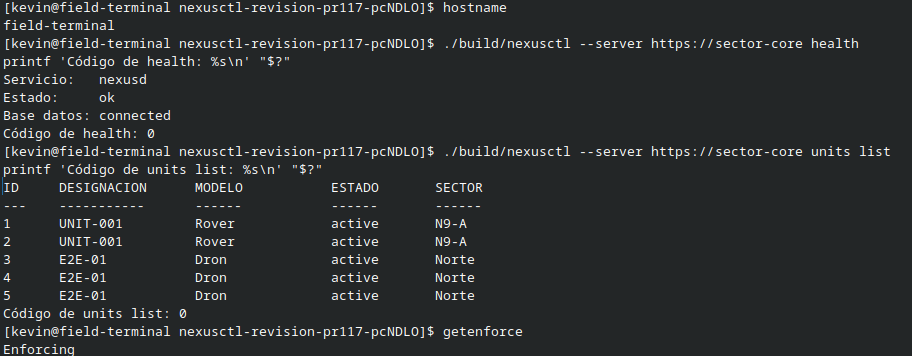
\includegraphics[width=0.88\textwidth]{images/E7_I72_01_health_units_rocky.png}
    \caption{Ejecución de \texttt{nexusctl} desde Rocky Linux operando contra la API HTTPS del sector.}
    \label{fig:e7_nexusctl}
\end{figure}

En la Figura~\ref{fig:e7_incidents_create} y Figura~\ref{fig:e7_incidents_val} se documenta exhaustivamente el subcomando de creación de incidentes (\texttt{nexusctl incidents create}) operando desde \texttt{field-terminal}:
\begin{itemize}[leftmargin=*]
    \item \textbf{Creación legítima en el sector (Figura~\ref{fig:e7_incidents_create}):} El operador invoca el comando con todos los argumentos mandatorios requeridos por la especificación: \texttt{--unit 6}, \texttt{--operator 1}, \texttt{--severity critical} y una descripción representativa. El cliente efectúa el \texttt{POST /api/v1/incidents} vía HTTPS validado con la CA, recibiendo la confirmación del servidor con el identificador asignado (\texttt{ID: 11}) y finalizando con código de retorno exitoso \texttt{0}.
    \item \textbf{Validación defensiva en el cliente (Figura~\ref{fig:e7_incidents_val}):} Si se omite alguno de los parámetros mandatorios (por ejemplo ejecutando únicamente con \texttt{--unit 6}), el cliente valida el formato antes de emitir ninguna conexión de red. Emite un mensaje de error descriptivo con la sintaxis requerida y retorna de forma inequívoca con \texttt{código 1} (\texttt{NEXUSCTL\_EXIT\_USAGE}), evitando generar carga superflua sobre la API.
\end{itemize}

\begin{figure}[H]
    \centering
    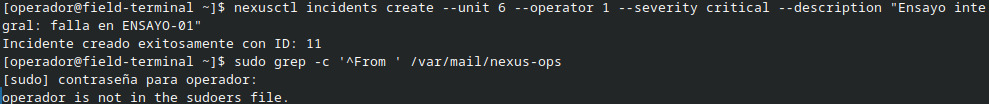
\includegraphics[width=0.92\textwidth]{images/E7_I74_01_crear_incidente.png}
    \caption{Creación confirmada de incidente crítico mediante \texttt{nexusctl} reportando ID 11.}
    \label{fig:e7_incidents_create}
\end{figure}

\begin{figure}[H]
    \centering
    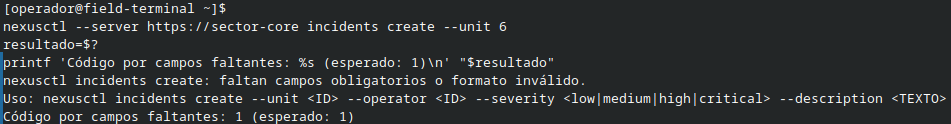
\includegraphics[width=0.92\textwidth]{images/E7_I74_02_crear_incidente_validacion.png}
    \caption{Validación previa en cliente: aborto inmediato sin conexión ante argumentos faltantes (código 1).}
    \label{fig:e7_incidents_val}
\end{figure}

En la Figura~\ref{fig:e7_incidents_close} y Figura~\ref{fig:e7_incidents_err} se comprueba el ciclo de cierre de incidentes (\texttt{nexusctl incidents close}) y el tratamiento diferenciado de códigos de error:
\begin{itemize}[leftmargin=*]
    \item \textbf{Cierre exitoso mediante PATCH (Figura~\ref{fig:e7_incidents_close}):} Al ejecutar \texttt{nexusctl incidents close 12}, el cliente emite la petición \texttt{PATCH} modificando el estado del incidente a \texttt{closed} y devolviendo código \texttt{0}. Inmediatamente después, se realiza una consulta de verificación vía \texttt{--json incidents list} exportada a archivo; un script en Python inspecciona el JSON confirmando que el incidente 12 figura con \texttt{"status": "closed"} y su respectiva marca temporal de actualización (\texttt{updated\_at}).
    \item \textbf{Gestión de incidentes inexistentes (Figura~\ref{fig:e7_incidents_err}):} Al intentar cerrar un identificador inexistente (\texttt{ID 999999}), la API retorna HTTP \texttt{404 Not Found}. El cliente interpreta la respuesta y emite el mensaje \texttt{"incidente 999999 no encontrado"}, saliendo con \texttt{código 2} (\texttt{NEXUSCTL\_EXIT\_API\_ERROR}), distinguiéndolo certeramente de un error de sintaxis (1), transporte (3) o certificados TLS (4).
\end{itemize}

\begin{figure}[H]
    \centering
    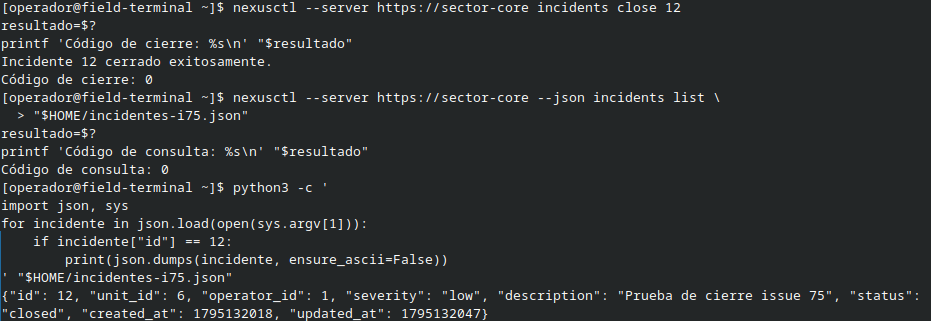
\includegraphics[width=0.92\textwidth]{images/E7_I75_01_cerrar_incidente.png}
    \caption{Cierre de incidente legítimo mediante PATCH y corroboración de estado \texttt{closed} en JSON.}
    \label{fig:e7_incidents_close}
\end{figure}

\begin{figure}[H]
    \centering
    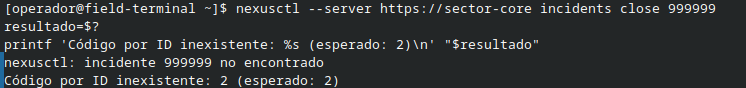
\includegraphics[width=0.92\textwidth]{images/E7_I75_02_cerrar_incidente_inexistente.png}
    \caption{Tratamiento riguroso de error de API: reporte de incidente no encontrado con código 2.}
    \label{fig:e7_incidents_err}
\end{figure}

% ==============================================================================
% SECCIÓN 8: ETAPA 08 — DESPLIEGUE AUTOMATIZADO Y PRUEBA INTEGRAL
% ==============================================================================
\section{Etapa 08 — Despliegue Automatizado, Idempotencia y Prueba Integral}

Para asegurar la reproducibilidad de la plataforma y evitar intervenciones manuales propensas a errores, se construyó el script de orquestación transaccional \textbf{\texttt{scripts/deploy.sh}}. La validación culmina con el ensayo integral de 14 pasos que recorre de punta a punta la plataforma operativa.

\subsection{Secuencia de Despliegue de \texttt{deploy.sh}}

La instalación requiere paquetes, caché de Conan, usuarios, directorios y montaje SFTP previamente preparados según \path{docs/installation.md}. En las actualizaciones se debe coordinar manualmente una ventana sin cargas ni clientes escribiendo: el script no implementa una pausa general de escrituras ni una instantánea atómica de toda la máquina.

\begin{enumerate}[leftmargin=*]
    \item \textbf{Validación de dependencias y privilegios:} Comprueba argumentos, privilegios, herramientas y paquetes disponibles en la caché local de Conan. Usa un bloqueo para excluir despliegues concurrentes y rechaza transacciones pendientes. No instala dependencias automáticamente ni realiza una comprobación específica de capacidad de disco antes del build.
    \item \textbf{Detección de primera instalación:} Distingue la ausencia de binario, configuración y unidad previos. Si encuentra una base existente sin instalación reconocida, exige revisión manual en lugar de borrarla. En una instalación nueva comprueba además los requisitos previos de usuarios, directorios y montaje SFTP.
    \item \textbf{Build independiente y pruebas:} Crea un directorio de compilación propio, configura y compila el código y ejecuta CTest en el entorno aislado de systemd. Si las pruebas fallan, termina antes de instalar archivos o cambiar servicios. Las configuraciones candidatas se toman del repositorio; no existe una fase separada de staging y validación integral de todas ellas.
    \item \textbf{Snapshot preventivo:} Conserva los archivos gestionados previos, enlaces, estados de servicios y una copia consistente de SQLite en \path{/var/backups/nexus/}. Incluye el certificado público de confianza local y registra las unidades que antes no existían. No contiene el árbol completo de evidencias, las claves de la CA ni toda la configuración de firewall, Postfix o montajes.
    \item \textbf{Instalación de binarios y configuración:} Reemplaza cada binario mediante escritura junto al destino y renombrado. Conserva \texttt{nexus.conf}; para otros archivos gestionados que difieren guarda una copia previa. El renombrado es atómico por archivo, no para el conjunto del despliegue.
    \item \textbf{Confianza local en la primera instalación:} Incorpora únicamente el certificado público de la CA al almacén de confianza de Ubuntu y ejecuta \texttt{update-ca-certificates}. No sustituye automáticamente una CA local distinta. Este paso no se ejecuta en las actualizaciones.
    \item \textbf{Unidades y servicios:} Instala las unidades y el script de backup, ejecuta \texttt{systemctl daemon-reload}, habilita nexus y el timer y reinicia nexus. Recarga Nginx o SSH si hay cambios pendientes. La activación final del timer queda para la confirmación.
    \item \textbf{Primer backup:} En una instalación nueva ejecuta \texttt{nexus-backup.service} tras comprobar HTTPS. En actualizaciones no genera un backup adicional para ocultar un historial fallido.
    \item \textbf{Validación y confirmación:} Ejecuta \texttt{health-check.sh} completo, incluidos los controles del backup. Solo el código \texttt{0} permite confirmar; se activa el timer, se persiste la fase final y se podan los snapshots confirmados antiguos.
    \item \textbf{Rollback ante fallos posteriores al snapshot:} Intenta restaurar los archivos, la base y los estados inventariados, conservando el error original si la recuperación se completa. En primera instalación retira archivos y habilitaciones nuevos e informa que no había una versión anterior; conserva PKI, datos y backups generados para revisión. Un rollback incompleto devuelve \texttt{11}. No se promete revertir los recursos que el snapshot no incluye.
\end{enumerate}

La secuencia inicial corregida cuenta con pruebas de regresión con destinos temporales y componentes simulados. Su ejecución completa en máquinas virtuales limpias fue validada empíricamente en el ensayo de la Guía de Instalación (Sección~\ref{sec:ensayo_maquinas_limpias}), mientras que la homologación por una persona ajena al equipo permanece asentada como criterio formal pendiente.

\subsection{Garantía de Idempotencia}

Un despliegue es \textbf{idempotente} si ejecutarlo múltiples veces consecutivas produce exactamente el mismo estado final estable que una sola ejecución. En \texttt{deploy.sh}, el proceso compila y prueba el código objetivo; sin embargo, al contrastar los artefactos y configuraciones candidatas contra los actualmente instalados, detecta si ya son idénticos. En tal caso, evita reemplazar archivos innecesariamente, no pisa bases de datos ni duplica reglas, concluyendo con código \texttt{0} e informando \textit{"sin cambios"}.

\subsection{Respuestas a Preguntas de Investigación}

\begin{pregunta}{¿Qué habría que guardar antes de instalar para poder volver atrás?}
    \textbf{Respuesta:} Debe capturarse una instantánea acotada a los elementos del sistema que el despliegue mutará: los ejecutables previos en \texttt{/usr/local/bin/}, los archivos de configuración en \texttt{/etc/nexus/}, los ficheros de unidad en \texttt{/etc/systemd/system/}, el estado de ejecución activo de los servicios, y una copia consistente de la base SQLite (\texttt{nexus.db}). No corresponde incluir el árbol completo de evidencias físicas (lo que insumiría tiempo y almacenamiento excesivo) ni paquetes del sistema operativo ajenos a la aplicación.
\end{pregunta}

\begin{pregunta}{¿Qué significa que un despliegue sea idempotente? ¿Qué pasa si se ejecuta dos veces seguidas?}
    \textbf{Respuesta:} Significa que aplicar la automatización una o diez veces sobre el mismo estado produce exactamente el mismo resultado final predecible, sin efectos colaterales acumulativos. Si se ejecuta dos veces consecutivas con la misma versión de código, el script realiza la compilación y pruebas, pero al verificar que los binarios y configuraciones del sistema coinciden con los candidatos, conserva los archivos idénticos y los datos. Sin embargo, vuelve a compilar, ejecutar pruebas y reiniciar nexus, por lo que cambian el PID y los tiempos de actividad. Sale con éxito (\texttt{código 0}) confirmando que el entorno ya está en el estado deseado.
\end{pregunta}

\begin{pregunta}{¿Por qué hay que recargar systemd después de instalar una unidad?}
    \textbf{Respuesta:} Porque \texttt{systemd} mantiene en memoria una representación interna en forma de grafo de dependencias de todas las unidades conocidas del sistema. Si se copia o modifica un archivo \texttt{.service} o \texttt{.timer} en el disco (\texttt{/etc/systemd/system/}), el daemon de inicialización no leerá los cambios de forma automática. Ejecutar \texttt{systemctl daemon-reload} le instruye reescanear los directorios de unidades y regenerar el árbol de dependencias sin necesidad de reiniciar el host.
\end{pregunta}

\begin{pregunta}{¿Qué parte del estado del sistema no puede revertir un rollback?}
    \textbf{Respuesta:} Los efectos secundarios que hayan trascendido hacia el exterior del host o asentado en registros persistentes: correos electrónicos ya despachados por Postfix a la red, peticiones de clientes externos que hayan sido procesadas durante la ventana en que la versión fallida estuvo viva, y las trazas históricas persistentes ya escritas en \texttt{journald} o en la auditoría del sistema operativo. Un rollback revierte binarios, configuraciones y la base de datos local, pero no puede deshacer interacciones con el mundo exterior.
\end{pregunta}

\begin{pregunta}{¿Qué debería hacer el script si lo ejecutan sin privilegios suficientes?}
    \textbf{Respuesta:} Debe comprobar de forma inmediata el identificador de usuario efectivo (\texttt{EUID == 0}) en la fase inicial de prevalidación. Si quien ejecuta no es \texttt{root}, debe abortar limpiamente emitiendo un mensaje de error explícito en \texttt{stderr} y finalizar con un código de salida no nulo preestablecido (en \texttt{deploy.sh}, \texttt{código 4}), sin intentar compilar, sin crear directorios temporales y sin alterar ningún archivo del sistema.
\end{pregunta}

\subsection{Evidencias de la Automatización del Despliegue}

En la Figura~\ref{fig:e8_prevalidacion} se exhibe la robustez de la prevalidación: ejecutar \texttt{deploy.sh} sin permisos de superusuario aborta de inmediato con \texttt{código 4}, y ejecutarlo ante dependencias ausentes en la caché local de Conan detiene el despliegue con \texttt{código 2} sin tocar la instalación.

\begin{figure}[H]
    \centering
    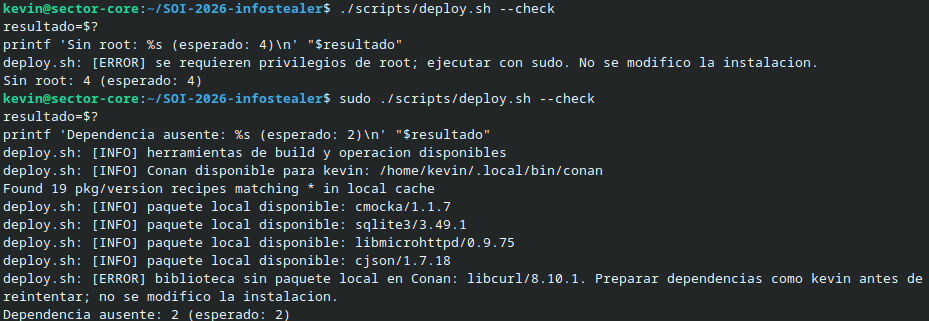
\includegraphics[width=0.88\textwidth]{images/E8_I78_01_prevalidacion.png}
    \caption{Prevalidación defensiva de \texttt{deploy.sh}: detención ante falta de privilegios o dependencias.}
    \label{fig:e8_prevalidacion}
\end{figure}

En la Figura~\ref{fig:e8_idempotencia} se demuestra la idempotencia mediante la prueba automatizada \texttt{test-deploy-idempotence.sh}: la segunda ejecución consecutiva detecta que no hay alteraciones requeridas, no duplica archivos y confirma que la base de datos permanece intacta.

\begin{figure}[H]
    \centering
    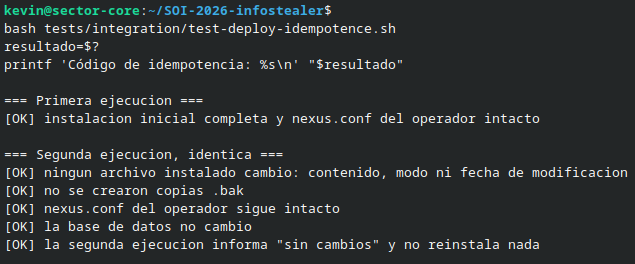
\includegraphics[width=0.88\textwidth]{images/E8_I84_02_idempotencia.png}
    \caption{Comprobación de idempotencia en despliegues sucesivos sin alteración de datos.}
    \label{fig:e8_idempotencia}
\end{figure}

En la Figura~\ref{fig:e8_rollback} se documenta el comportamiento de reversión automática mediante \texttt{test-deploy-rollback.sh}: al simular la instalación de un binario corrupto que hace fallar el health check posterior, el orquestador aborta, restituye el binario sano precedente (v1) desde el snapshot y devuelve \texttt{código 10}.

\begin{figure}[H]
    \centering
    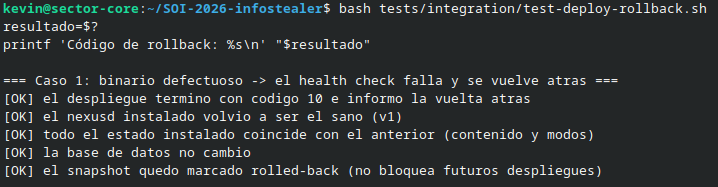
\includegraphics[width=0.88\textwidth]{images/E8_I85_03_rollback.png}
    \caption{Ejecución automática de rollback restaurando la versión sana previa ante fallo de validación.}
    \label{fig:e8_rollback}
\end{figure}

\subsection{Verificación Experimental de la Guía de Instalación en Máquinas Limpias (Issue \#86 / E8-10)}
\label{sec:ensayo_maquinas_limpias}

Como parte de los requerimientos de la Etapa 08 y el seguimiento de la \textbf{Issue \#86} (\textit{E8-10: Documento de instalación para una persona ajena al equipo}), se estructuró la guía paso a paso \path{docs/installation.md} (formalizada en la PR \#135 tras superar la validación sintáctica de sus 38 bloques Bash y comprobación de rutas y enlaces). 

Para verificar empíricamente la reproducibilidad técnica de dicho instructivo fuera de los entornos de desarrollo preexistentes, se llevó a cabo un \textbf{ensayo de instalación integral desde cero sobre dos máquinas virtuales nuevas e independientes} creadas en VirtualBox:
\begin{itemize}[leftmargin=*]
    \item \textbf{Nodo Servidor (\texttt{sector-core}):} Ubuntu Server 26.04.1 LTS x86\_64 (IP de ensayo: \texttt{192.168.56.101}).
    \item \textbf{Nodo Cliente (\texttt{field-terminal}):} Rocky Linux 10.2 x86\_64 (IP de ensayo: \texttt{192.168.56.102}).
    \item \textbf{Versión de Código Evaluada:} Commit \texttt{44048725481ee120888afb1904fa8b7704843807} (rama \texttt{TP3}).
\end{itemize}

El ensayo cubrió el aprovisionamiento de dependencias, compilación, creación de usuarios, configuración del chroot SFTP, confianza en la CA raíz, despliegue de \texttt{nexusd}, generación del primer backup y validación perimetral completa. A continuación se presentan las 11 evidencias documentadas durante la ejecución de las fases de la guía:

\subsubsection*{1. Identificación de Entorno y Verificación de Commit}
En las Figuras~\ref{fig:e8_clean_so_core} y~\ref{fig:e8_clean_so_term} se constata el arranque de ambas máquinas virtuales en estado inicial, verificando la versión del kernel, la distribución de sistema operativo y la alineación estricta al commit de evaluación en la rama \texttt{TP3}.

\begin{figure}[H]
    \centering
    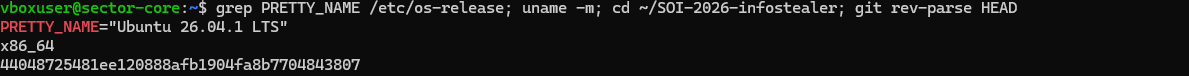
\includegraphics[width=0.88\textwidth]{images/01_sector-core_SO-y-commit.png}
    \caption{Identificación de sistema operativo, arquitectura x86\_64 y commit en \texttt{sector-core}.}
    \label{fig:e8_clean_so_core}
\end{figure}

\begin{figure}[H]
    \centering
    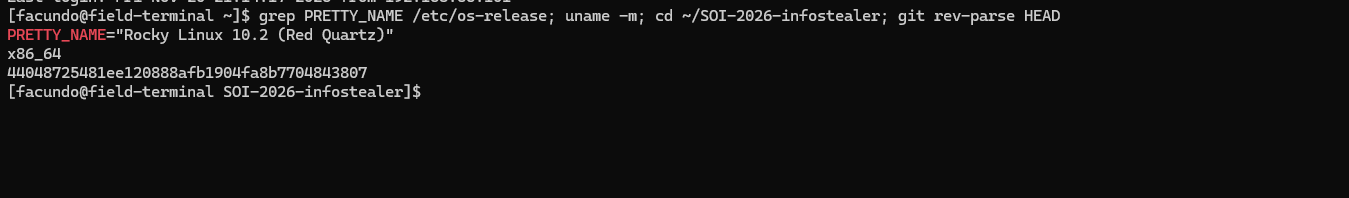
\includegraphics[width=0.88\textwidth]{images/02_field-terminal_SO-y-commit.png}
    \caption{Identificación de sistema operativo, arquitectura y commit en \texttt{field-terminal} (Rocky Linux 10.2).}
    \label{fig:e8_clean_so_term}
\end{figure}

\subsubsection*{2. Despliegue Inicial, Confianza TLS y Primer Backup en \texttt{sector-core}}
Tras ejecutar la secuencia de instalación inicial (registrada en \path{~/deploy-first.log} con retorno \texttt{0}), el orquestador activó automáticamente \texttt{nexus-backup.service} para generar el primer backup de contingencia antes de permitir tráfico externo. En la Figura~\ref{fig:e8_clean_backup} se exhibe la confirmación del archivo de backup verificado en \path{/var/backups/nexus/}. En la Figura~\ref{fig:e8_clean_tls_health} se corrobora la validación criptográfica de la cadena con \texttt{openssl verify -CAfile} positiva (\texttt{OK}), la huella SHA-256 de la CA local y la ejecución exitosa de \texttt{health-check.sh} con código de salida \texttt{0} (paso A6 de la guía).

\begin{figure}[H]
    \centering
    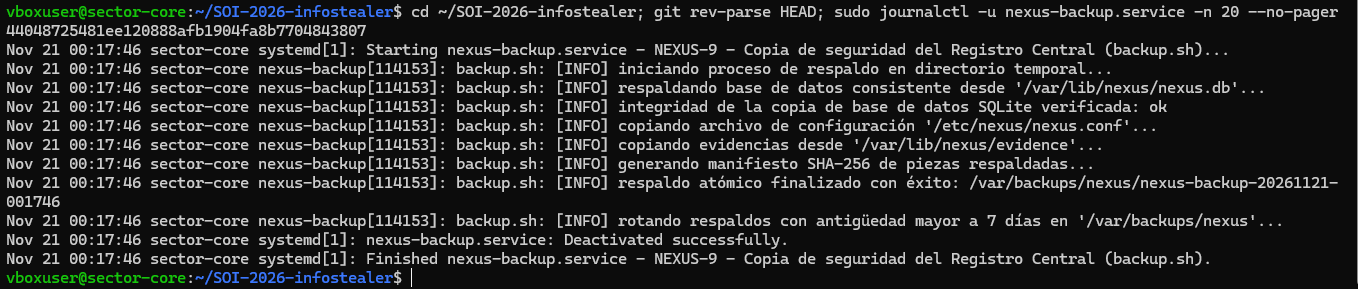
\includegraphics[width=0.88\textwidth]{images/03_sector-core_primer-backup.png}
    \caption{Generación y validación del primer backup de contingencia tras la primera instalación en \texttt{sector-core}.}
    \label{fig:e8_clean_backup}
\end{figure}

\begin{figure}[H]
    \centering
    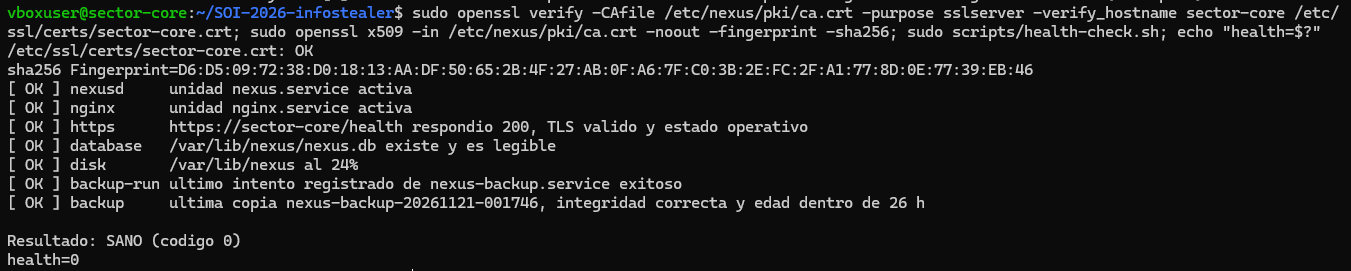
\includegraphics[width=0.88\textwidth]{images/04_sector-core_certificado-y-health.png}
    \caption{Validación positiva de OpenSSL con la CA raíz del laboratorio y comprobación de salud (\texttt{health 0}).}
    \label{fig:e8_clean_tls_health}
\end{figure}

\subsubsection*{3. Confinamiento de Red y Puertos en el Servidor}
En la Figura~\ref{fig:e8_clean_puertos} se verifica el estado operativo de los demonios supervisados por systemd (\texttt{nexus}, \texttt{nginx}, \texttt{ssh}), la inspección de sockets en escucha con \texttt{ss -tulpn} —evidenciando que el backend \texttt{nexusd} escucha exclusivamente en el lazo cerrado \texttt{127.0.0.1:8080} mientras Nginx publica el puerto 443— y el estado activo del cortafuegos \texttt{ufw} autorizando únicamente SSH y HTTPS (paso A7 de la guía).

\begin{figure}[H]
    \centering
    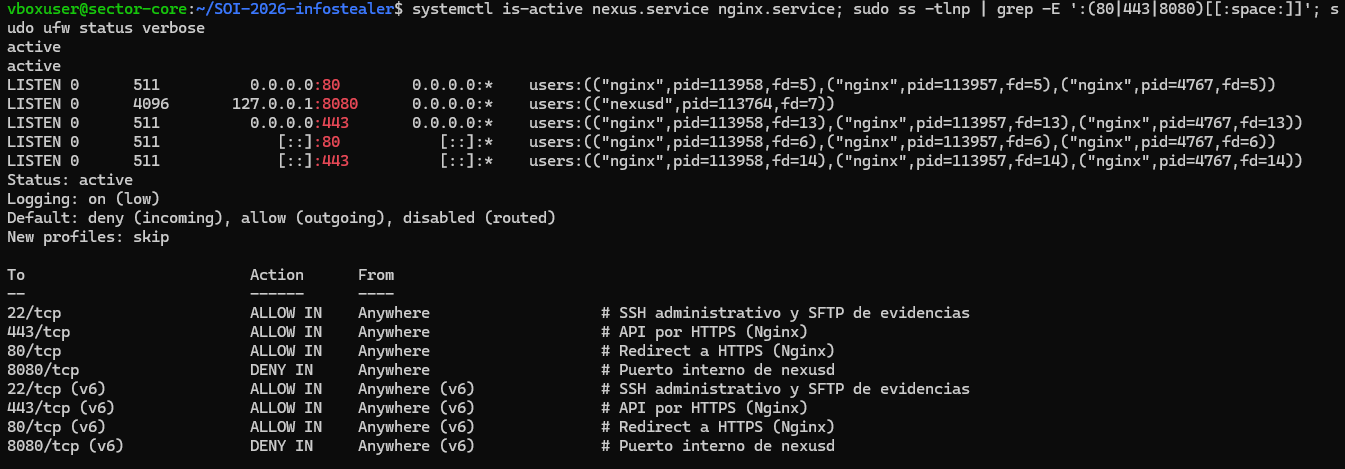
\includegraphics[width=0.88\textwidth]{images/05_sector-core_servicios-puertos-firewall.png}
    \caption{Servicios en ejecución, sockets activos (\texttt{127.0.0.1:8080} confinado) y reglas de \texttt{ufw} en \texttt{sector-core}.}
    \label{fig:e8_clean_puertos}
\end{figure}

\subsubsection*{4. Consumo de API por Cliente Nativo sobre HTTPS}
Desde \texttt{field-terminal}, se ejecutó \texttt{nexusctl health} contra el servidor. Como se observa en la Figura~\ref{fig:e8_clean_client_health}, la biblioteca \texttt{libcurl} resolvió el apretón de manos TLS de forma transparente gracias a la previa incorporación del certificado de la CA raíz en el almacén de Rocky Linux (\path{/etc/pki/ca-trust/source/anchors/}), retornando la respuesta JSON de salud sin requerir parámetros de evasión insegura (pasos B3 y B4).

\begin{figure}[H]
    \centering
    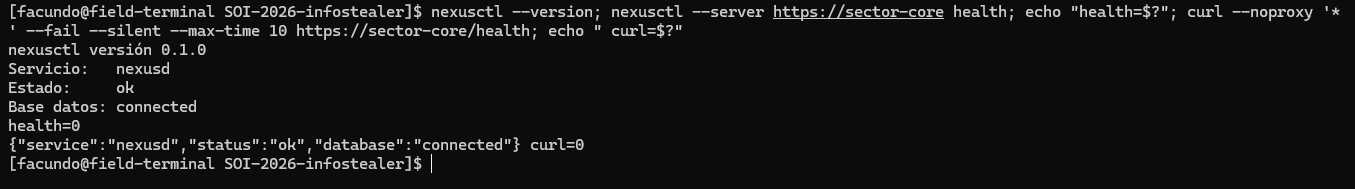
\includegraphics[width=0.88\textwidth]{images/06_field-terminal_nexusctl-health-HTTPS.png}
    \caption{Consulta de salud desde \texttt{field-terminal} con \texttt{nexusctl} verificando canal seguro HTTPS y código de retorno \texttt{0}.}
    \label{fig:e8_clean_client_health}
\end{figure}

\subsubsection*{5. Transferencia de Evidencias, Integridad SHA-256 y Confinamiento SFTP}
Se procedió a transferir un archivo binario de prueba mediante el usuario restringido \texttt{nexus\_evidence}. En la Figura~\ref{fig:e8_clean_sftp_put} se constata la transferencia SFTP exitosa con código de retorno \texttt{0}. En la Figura~\ref{fig:e8_clean_sftp_dest} se comprueba en \texttt{sector-core} que el hash SHA-256 calculado en destino sobre \path{/var/lib/nexus/evidence/incoming/} coincide idénticamente con el generado en origen (\texttt{69f2bc8e3981...}). Finalmente, en la Figura~\ref{fig:e8_clean_sftp_noshell} se valida el rechazo tajante de sesiones interactivas: cualquier intento de apertura de terminal SSH rechaza la conexión con el mensaje restrictivo \textit{"This service allows sftp connections only"} (paso B6 de la guía).

\begin{figure}[H]
    \centering
    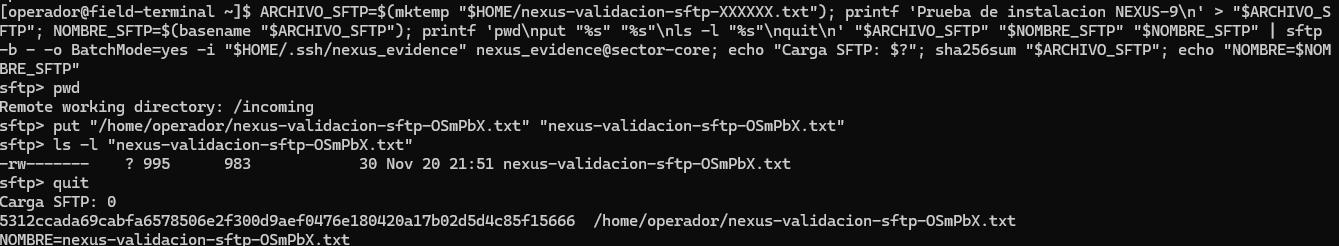
\includegraphics[width=0.88\textwidth]{images/07_field-terminal_carga-SFTP.png}
    \caption{Carga interactiva de archivo de prueba vía SFTP hacia \texttt{sector-core} con código de salida \texttt{0}.}
    \label{fig:e8_clean_sftp_put}
\end{figure}

\begin{figure}[H]
    \centering
    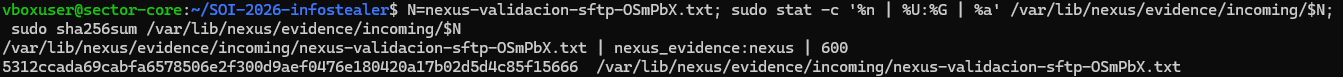
\includegraphics[width=0.88\textwidth]{images/08_sector-core_SFTP-checksum-y-modo.png}
    \caption{Verificación de coincidencia de checksum SHA-256 en \texttt{incoming} y revisión de permisos del archivo depositado.}
    \label{fig:e8_clean_sftp_dest}
\end{figure}

\begin{figure}[H]
    \centering
    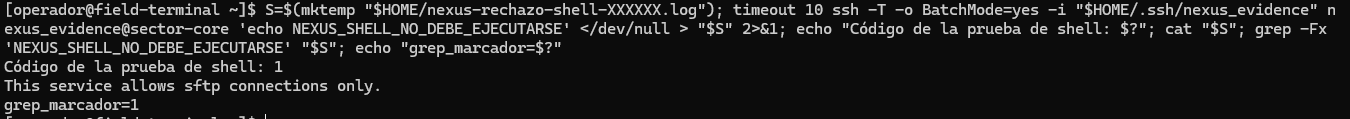
\includegraphics[width=0.88\textwidth]{images/09_field-terminal_rechazo-de-shell.png}
    \caption{Rechazo estricto de shell interactiva para el usuario de evidencias \texttt{nexus\_evidence}.}
    \label{fig:e8_clean_sftp_noshell}
\end{figure}

\subsubsection*{6. Operación de Campo: Unidades, Evidencias y Aislamiento Perimetral}
En la Figura~\ref{fig:e8_clean_op_evidence} se aprecia la actividad efectuada bajo la cuenta sin privilegios \texttt{operador} en \texttt{field-terminal}: se dio de alta la unidad táctica \texttt{ENSAYO-20261121-003401} mediante \texttt{nexusctl} y se asoció la evidencia previamente transferida registrando su hash criptográfico. Por último, en la Figura~\ref{fig:e8_clean_op_blocked} se demuestra el éxito del control perimetral (parte C de la guía): mientras que \texttt{nexusctl health} opera con código \texttt{0} sobre el puerto 443, el intento de acceso directo al puerto backend \texttt{192.168.56.101:8080} es descartado por el firewall, provocando que \texttt{curl} expire por tiempo de espera y finalice con código de error \texttt{28}.

\begin{figure}[H]
    \centering
    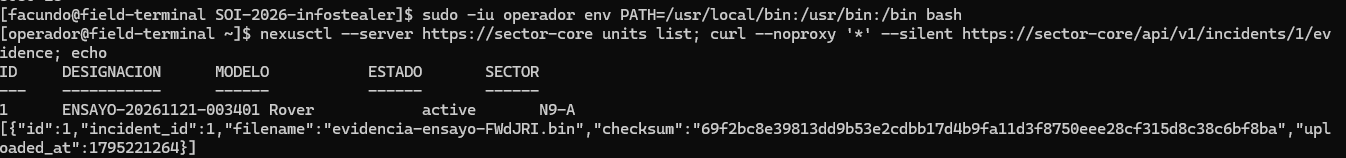
\includegraphics[width=0.88\textwidth]{images/10_field-terminal_operador-unidad-y-evidencia.png}
    \caption{Operación desde \texttt{field-terminal}: alta de unidad y registro de evidencia asociada con hash criptográfico.}
    \label{fig:e8_clean_op_evidence}
\end{figure}

\begin{figure}[H]
    \centering
    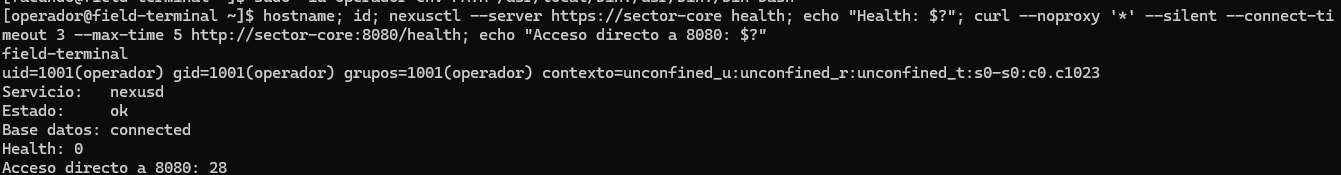
\includegraphics[width=0.88\textwidth]{images/11_field-terminal_operador-health-y-puerto-8080-bloqueado.png}
    \caption{Consulta nominal HTTPS (código \texttt{0}) y confirmación de puerto 8080 perimetralmente bloqueado (código 28 de curl).}
    \label{fig:e8_clean_op_blocked}
\end{figure}

\subsubsection*{Análisis de Diferencias Operativas y Hallazgos Técnicos}

La ejecución del ensayo permitió identificar discrepancias operativas y hallazgos técnicos de relevancia que enriquecen la documentación y perfilan los límites de la guía:

\begin{enumerate}[leftmargin=*]
    \item \textbf{Modo de Permisos en Transferencia SFTP Manual vs. Script Oficial:} En el ensayo interactivo manual (Figura~\ref{fig:e8_clean_sftp_dest}), el archivo subido mediante el comando \texttt{put} de \texttt{sftp} quedó en el destino con permisos \texttt{0600} en lugar de los \texttt{0640} descriptos en el paso B6 de la guía. Esto ocurre porque el comando interactivo \texttt{sftp} preserva el modo del archivo temporal en origen generado con \texttt{mktemp} (\texttt{0600}). En contraste, cuando la carga se efectúa mediante el script automatizado \texttt{upload-evidence.sh} (paso B8), el script se encarga explícitamente de normalizar la máscara a \texttt{0640} con pertenencia al grupo \texttt{nexus}, asegurando que el demonio lector disponga de acceso. Se constata la conveniencia de corregir la redacción del paso B6 en \path{docs/installation.md} para explicitar dicho comportamiento.
    \item \textbf{Destino de Entrega Local en Notificaciones Postfix:} Al registrar un incidente crítico, el demonio \texttt{nexusd} asentó en su registro \texttt{entrega=OK} para el destinatario \texttt{operadores@nexus9.local}. Sin embargo, el mensaje no se encontró disponible en el buzón local \path{/var/mail/nexus-ops} ni en la cola activa de Postfix debido a que el dominio \texttt{nexus9.local} no se hallaba explícitamente listado en la directiva \texttt{mydestination} de \path{/etc/postfix/main.cf}. La entrega interna requiere homogeneizar dicha directiva en la configuración del agente de transporte.
    \item \textbf{Entorno de Ejecución del Operador de Campo:} La guía instruye la conmutación al usuario operador mediante \texttt{su - operador}. Al utilizarse en el ensayo el comando \texttt{sudo -iu operador}, la variable de entorno \texttt{PATH} predeterminada por la configuración PAM de Rocky Linux excluyó el directorio \path{/usr/local/bin}, requiriendo invocación calificada o la debida exportación en el archivo \path{.bashrc}.
    \item \textbf{Adaptaciones de Red y Clonación:} Para el laboratorio del ensayo se asignó la subred privada con IPs \texttt{192.168.56.101} y \texttt{192.168.56.102} (ajustando consecuentemente las extensiones SAN del certificado y la variable \texttt{NEXUS\_SERVER\_IP}), y la clonación del repositorio se realizó a partir de un paquete git empaquetado (\textit{bundle}), evitando requerir conectividad hacia repositorios externos privados durante la preparación.
\end{enumerate}

\subsubsection*{Estado de Cumplimiento respecto al Criterio de la Consigna}

A partir de los resultados obtenidos, es imperativo distinguir entre la viabilidad técnica demostrada y el criterio formal de aprobación fijado por la cátedra:
\begin{itemize}[leftmargin=*]
    \item \textbf{Viabilidad Técnica Demostrada:} El ensayo constata fehacientemente que las instrucciones de \path{docs/installation.md} y los scripts de orquestación son reproducibles desde cero en sistemas operativos vírgenes: el despliegue concluye con éxito, los servicios se inician bajo supervisión de systemd, los cortafuegos y políticas MAC de SELinux operan en modo restrictivo (\textit{Enforcing}), las transferencias SFTP se enjaulan correctamente y el cliente C opera sin anomalías sobre HTTPS.
    \item \textbf{Criterio de Cierre Formal Pendiente (Issue \#86):} La consigna de la cátedra estipula textualmente que \textit{"Una persona ajena al equipo puede instalar el sector siguiendo la documentación"}. Dado que este ensayo fue conducido internamente por integrantes del equipo de desarrollo (Facundo asistido por un agente IA mediante SSH), \textbf{el criterio de cierre definitivo de la Issue \#86 permanece formalmente abierto}. La acreditación final requerirá que un evaluador independiente sin intervención de los autores registre su nombre, fecha, commit y reporte de observaciones sobre un entorno limpio.
\end{itemize}

\subsection{Recorrido Paso a Paso de la Prueba Integral (14 Pasos)}
\label{sec:integral}

La evaluación final del sector siguió un guion estandarizado y reproducible ejecutado en tiempo real con ambos nodos interconectados. A continuación se presenta cada uno de los 14 pasos junto a su respectiva evidencia experimental ampliada:

\subsubsection*{Paso 1 · Inicio de Sesión de Operador en Rocky Linux}
La operación comienza en \texttt{field-terminal} iniciando sesión con el usuario estándar \texttt{operador} (UID 1001), carente de privilegios administrativos en \texttt{sudoers}. Esto valida que las herramientas de interacción y monitoreo de campo no requieren privilegios de \texttt{root} para su funcionamiento cotidiano.

\begin{figure}[H]
    \centering
    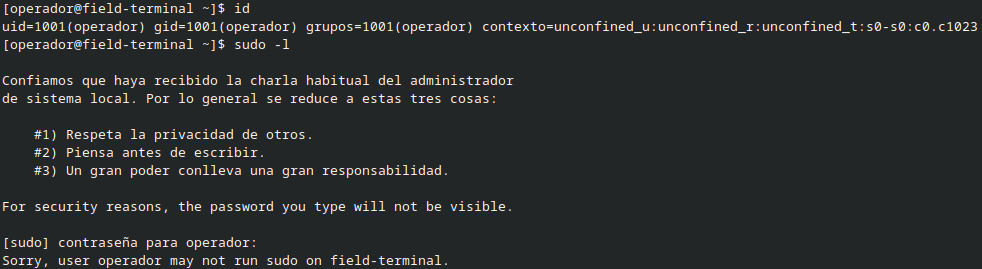
\includegraphics[width=0.94\textwidth]{images/INTEGRAL_I90_P01_operador_sin_privilegios.png.jpeg}
    \caption{Paso 1: Inicio de sesión interactiva con el usuario sin privilegios administrativos en \texttt{field-terminal}.}
    \label{fig:int_p1}
\end{figure}

\subsubsection*{Paso 2 · Verificación de Salud Perimetral con \texttt{nexusctl}}
El operador comprueba el estado global del sector mediante \texttt{nexusctl health}. El cliente en C realiza la petición HTTPS contra \texttt{https://sector-core/health}, validando el certificado mediante la CA de laboratorio instalada en el almacén de confianza del sistema, recibiendo la respuesta JSON y retornando con código de salida \texttt{0}.

\begin{figure}[H]
    \centering
    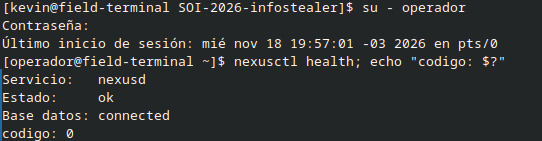
\includegraphics[width=0.94\textwidth]{images/INTEGRAL_I90_P02_health_https_codigo0.png.jpeg}
    \caption{Paso 2: Comprobación de salud perimetral vía HTTPS con validación de certificado (código 0).}
    \label{fig:int_p2}
\end{figure}

\subsubsection*{Paso 3 · Registro y Listado de Nueva Unidad Operativa}
Se envía una solicitud de alta de unidad (\texttt{POST /api/v1/units}) y se comprueba la persistencia consultando el listado estructurado mediante \texttt{nexusctl units list}, verificando que la cadena completa de transporte, proxy Nginx, daemon \texttt{nexusd} y almacenamiento SQLite funciona coordinadamente.

\begin{figure}[H]
    \centering
    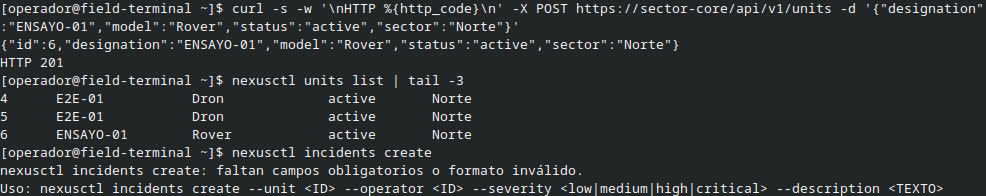
\includegraphics[width=0.94\textwidth]{images/INTEGRAL_I90_P03_creacion_unidad_y_listado.png.jpeg}
    \caption{Paso 3: Creación de unidad operativa y listado de confirmación mediante \texttt{nexusctl units list}.}
    \label{fig:int_p3}
\end{figure}

\subsubsection*{Paso 4 · Creación de Incidente Crítico}
El operador registra un nuevo incidente asignando severidad \texttt{critical} (\texttt{nexusctl incidents create --unit 6 --operator 1 --severity critical --description "Ensayo integral: falla en ENSAYO-01"}). La API genera el identificador único (\texttt{ID: 11}) y programa la notificación correspondiente.

\begin{figure}[H]
    \centering
    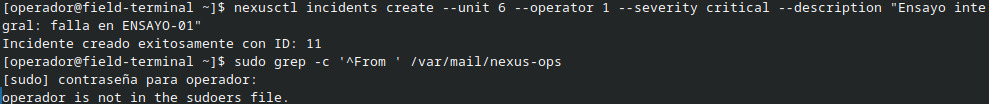
\includegraphics[width=0.94\textwidth]{images/INTEGRAL_I90_P04_creacion_incidente_critico.png.jpeg}
    \caption{Paso 4: Alta de incidente crítico disparando la cadena de alerta operativa con ID generado.}
    \label{fig:int_p4}
\end{figure}

\subsubsection*{Pasos 5 y 6 · Carga SFTP Enjaulada y Asociación de Evidencia con SHA-256}
Se ejecuta el script \texttt{upload-evidence.sh}: en el Paso 5, el archivo binario de evidencia se transfiere por SFTP autenticado con par de claves SSH hacia el directorio \texttt{/incoming} de la jaula chroot del usuario \texttt{nexus\_evidence}. En el Paso 6, el script calcula el hash SHA-256 del fichero y lo asocia formalmente al incidente vía API REST, validando concordancia criptográfica.

\begin{figure}[H]
    \centering
    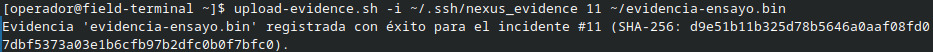
\includegraphics[width=0.94\textwidth]{images/INTEGRAL_I90_P05-P06_carga_y_registro_evidencia.png.jpeg}
    \caption{Pasos 5 y 6: Transferencia SFTP enjaulada y registro de evidencia con verificación de suma SHA-256.}
    \label{fig:int_p5_6}
\end{figure}

\subsubsection*{Paso 7 · Comprobación de Notificación Interna en Buzón Local}
Se inspecciona el buzón de correo local \texttt{/var/mail/nexus-ops} en \texttt{sector-core}, confirmando que el subsistema Postfix confinado en loopback entregó efectivamente el mensaje de alerta derivado del incidente crítico registrado en el Paso 4.

\begin{figure}[H]
    \centering
    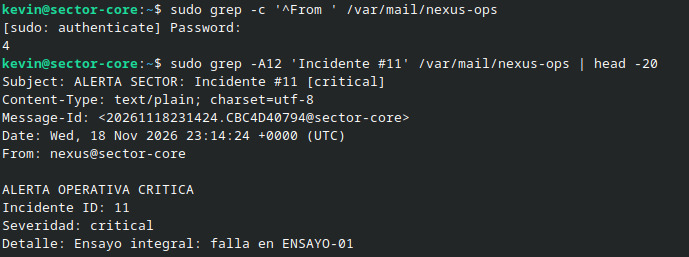
\includegraphics[width=0.94\textwidth]{images/INTEGRAL_I90_P07_notificacion_buzon_local.png.jpeg}
    \caption{Paso 7: Verificación de entrega de la notificación crítica en el buzón local \texttt{/var/mail/nexus-ops}.}
    \label{fig:int_p7}
\end{figure}

\subsubsection*{Paso 8 · Inspección de Eventos de Auditoría vía API}
El operador ejecuta una consulta HTTP desde \texttt{field-terminal} (consumiendo el endpoint \texttt{GET /api/v1/audit} mediante \texttt{curl}), verificando la lista estructurada de eventos registrados en la tabla de auditoría (altas de unidades, asociaciones de evidencia y notificaciones críticas) con sus correspondientes atributos de actor, acción, recurso, resultado y marca temporal.

\begin{figure}[H]
    \centering
    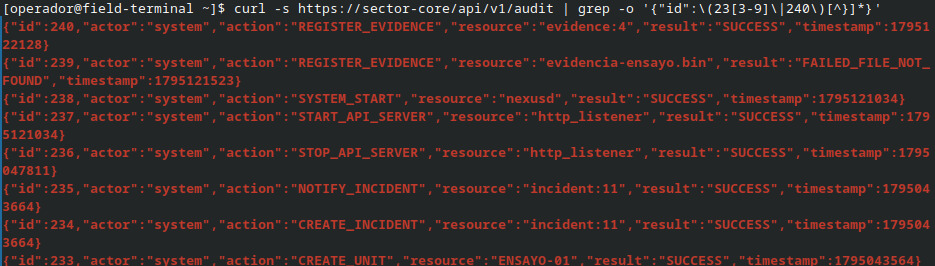
\includegraphics[width=0.94\textwidth]{images/INTEGRAL_I90_P08_eventos_auditoria.png.jpeg}
    \caption{Paso 8: Consulta de eventos de auditoría desde \texttt{field-terminal} reflejando las operaciones registradas.}
    \label{fig:int_p8}
\end{figure}

\subsubsection*{Pasos 9 y 10 · Caída Forzada de \texttt{nexusd} (\texttt{kill -9}) y Recuperación por Systemd}
En el Paso 9, se envía una señal letal \texttt{SIGKILL} al proceso principal de \texttt{nexusd}. En el Paso 10, se demuestra que el supervisor \texttt{systemd} detecta la interrupción anómala y aplica la directiva \texttt{Restart=on-failure}, aguardando el retardo configurado (\texttt{RestartSec=2s}) antes de reiniciar el demonio automáticamente con un nuevo PID, sin requerir intervención manual.

\begin{figure}[H]
    \centering
    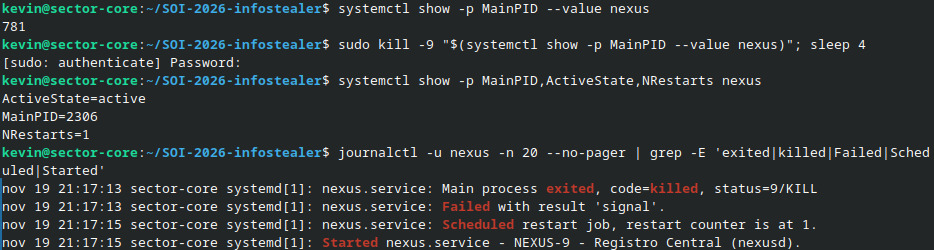
\includegraphics[width=0.94\textwidth]{images/INTEGRAL_I90_P09-P10_caida_y_recuperacion_systemd.png.jpeg}
    \caption{Pasos 9 y 10: Finalización abrupta (\texttt{kill -9}) y recuperación automática autónoma gobernada por Systemd.}
    \label{fig:int_p9_10}
\end{figure}

\subsubsection*{Paso 11 · Generación de Backup Consistente con Manifiesto}
Se ejecuta \texttt{scripts/backup.sh}, el cual realiza una copia en caliente consistente de la base SQLite utilizando la API de backup atómico (modo WAL), empaqueta el árbol de evidencias y genera un archivo de manifiesto criptográfico con sumas SHA-256.

\begin{figure}[H]
    \centering
    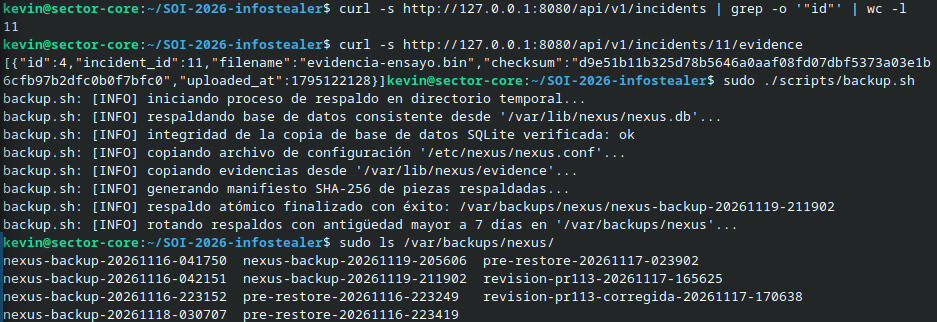
\includegraphics[width=0.94\textwidth]{images/INTEGRAL_I90_P11_generacion_backup.png.jpeg}
    \caption{Paso 11: Generación de respaldo consistente, empaquetado de evidencias y cálculo de sumas SHA-256.}
    \label{fig:int_p11}
\end{figure}

\subsubsection*{Paso 12 · Pérdida Controlada de Información}
Para simular un incidente de pérdida de datos, se eliminan intencionalmente el archivo de base de datos \texttt{nexus.db} y los archivos contenidos en el subdirectorio \texttt{incoming} de evidencias (conservando las rutas de directorios). La consulta posterior a la API refleja la pérdida de los registros previos, observándose una respuesta con cero incidentes en el sector y demostrando la necesidad de ejecutar el procedimiento de restauración.

\begin{figure}[H]
    \centering
    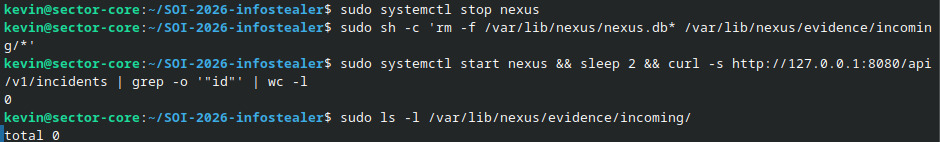
\includegraphics[width=0.94\textwidth]{images/INTEGRAL_I90_P12_perdida_informacion.png.jpeg}
    \caption{Paso 12: Simulación de pérdida de datos eliminando la base SQLite y los archivos de \texttt{incoming}, observándose una respuesta con cero incidentes.}
    \label{fig:int_p12}
\end{figure}

\subsubsection*{Paso 13 · Restauración Íntegra con Validación de Integridad}
Se invoca \texttt{scripts/restore.sh} apuntando al snapshot generado en el Paso 11. El script valida la integridad de cada archivo contra el manifiesto SHA-256 antes de transferir datos, restaura la base SQLite y reconstruye el árbol de evidencias con los permisos correctos.

\begin{figure}[H]
    \centering
    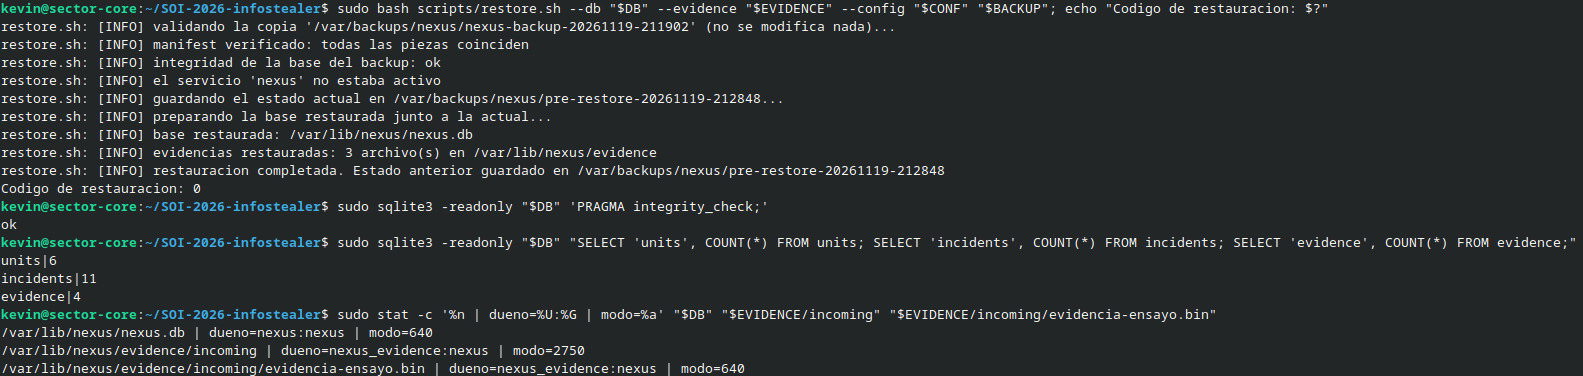
\includegraphics[width=0.94\textwidth]{images/INTEGRAL_I90_P13_restauracion_integridad.png.jpeg}
    \caption{Paso 13: Restauración completa de la plataforma con verificación previa de integridad criptográfica.}
    \label{fig:int_p13}
\end{figure}

\subsubsection*{Paso 14 · Verificación Final del Sector con \texttt{nexusctl}}
Desde \texttt{field-terminal}, el operador consulta nuevamente los endpoints de unidades e incidentes con \texttt{nexusctl}. Se corrobora fehacientemente que la unidad creada en el Paso 3 y el incidente crítico del Paso 4 persisten sin alteración, certificando el éxito total del circuito.

\begin{figure}[H]
    \centering
    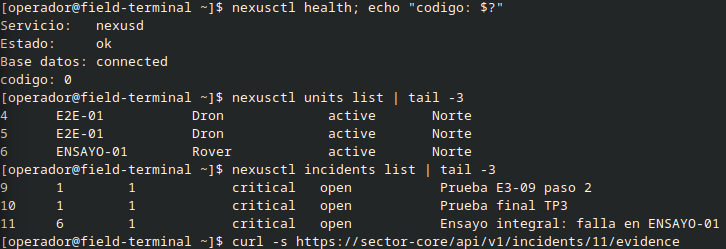
\includegraphics[width=0.94\textwidth]{images/INTEGRAL_I90_P14_verificacion_datos_recuperados.png.jpeg}
    \caption{Paso 14: Verificación final de consistencia constatando la recuperación íntegra de entidades operativas.}
    \label{fig:int_p14}
\end{figure}

% ==============================================================================
% SECCIÓN 9: ESCENARIOS DE FALLA OBLIGATORIOS
% ==============================================================================
\section{Escenarios de Falla Obligatorios}

El sistema fue diseñado y evaluado bajo condiciones adversas, demostrando la capacidad de supervivencia y diagnóstico autónomo ante los tres escenarios de contingencia obligatorios fijados por la cátedra.

\subsection{Demostración de los Escenarios de Falla Obligatorios}

\begin{enumerate}[leftmargin=*]
    \item \textbf{Falla 1 · Proceso Terminado Abruptamente (\texttt{kill -9}):}
    Se emitió una señal no interceptable \texttt{SIGKILL} al proceso de \texttt{nexusd}. El kernel finalizó el proceso de inmediato. El supervisor \texttt{systemd} detectó la pérdida del PID principal, aguardó el tiempo de retardo configurado (\texttt{RestartSec=2s}) y reanudó automáticamente el servicio con un nuevo PID, registrando el evento en journald con \texttt{code=killed, status=9/KILL} (documentado experimentalmente en la Figura~\ref{fig:e4_recuperacion} y en los Pasos 9 y 10 de la prueba integral).
    \item \textbf{Falla 2 · Base de Datos No Disponible (EC-02):}
    Al interrumpirse el acceso al archivo SQLite de forma imprevista mientras el demonio sigue en ejecución, \texttt{nexusd} atrapa la condición de fallo a nivel de su capa de persistencia sin abortar el proceso. Emite respuestas HTTP semánticas \texttt{503 Service Unavailable} (\texttt{database\_unavailable}) en todos los endpoints que dependen del almacenamiento (no únicamente en \texttt{/health}), y al restablecerse el acceso reanuda el servicio con código 200 conservando el mismo PID (documentado experimentalmente en la Figura~\ref{fig:falla2_db}).
    \item \textbf{Falla 3 · Pérdida Catastrófica de Información:}
    Se eliminó intencionalmente el archivo de base de datos \texttt{nexus.db} y los archivos físicos de evidencia. Siguiendo el procedimiento documentado, se ejecutó \texttt{restore.sh} recuperando la totalidad de unidades, operadores, incidentes y sumas de control desde el último backup consistente (documentado en la Figura~\ref{fig:e5_restauracion} y en los Pasos 11 al 13).
\end{enumerate}

\subsection{Evidencia Experimental: Falla 2 · Base de Datos No Disponible (EC-02 / Issue \#88)}

En la Figura~\ref{fig:falla2_db} se documenta la ejecución automatizada del guion de contingencia \texttt{test-database-unavailable.py} (en \texttt{tests/integration/}), ejecutado como un ensayo controlado sobre una instancia real del binario \texttt{nexusd} con una base de datos temporal apartada durante la prueba (ejecutada en espacio de usuario, sin privilegios \texttt{sudo} y sin alterar el servicio en producción instalado \texttt{nexus.service}):
\begin{itemize}[leftmargin=*]
    \item \textbf{Estado inicial nominal:} La API arranca atendiendo peticiones con código HTTP \texttt{200 OK} bajo el proceso principal con identificador \texttt{PID 1552}.
    \item \textbf{Aislamiento defensivo ante pérdida de base:} Al apartar temporalmente el archivo de base de datos mientras el demonio permanece en ejecución continua, \texttt{nexusd} atrapa los fallos de consulta de SQLite a nivel de capa de datos. En lugar de abortar abruptamente (\textit{crash}) o emitir excepciones no controladas, el servidor intercepta el error y responde con código semántico \textbf{HTTP 503 Service Unavailable} y cuerpo \texttt{database\_unavailable} en la totalidad de rutas dependientes (\texttt{/health}, \texttt{/api/v1/health}, \texttt{/api/v1/units}, \texttt{/api/v1/operators}, \texttt{/api/v1/incidents}, evidencias y auditoría).
    \item \textbf{Recuperación transparente sin reinicio de proceso:} Una vez restituido el archivo de base de datos, el servicio reanuda de inmediato el despacho de respuestas HTTP \texttt{200 OK} con los datos preexistentes intactos, demostrando que \textbf{conservó el mismo PID 1552} durante todo el incidente y finalizando la prueba con código de salida \texttt{0} (\texttt{Código de demostración EC-02: 0}).
\end{itemize}

\begin{figure}[H]
    \centering
    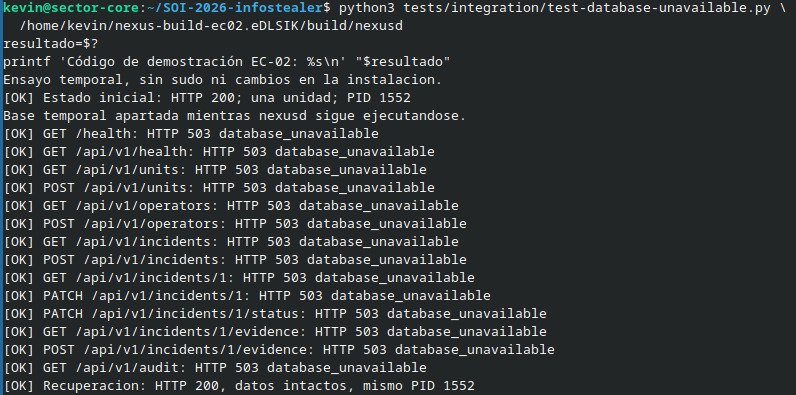
\includegraphics[width=0.92\textwidth]{images/FALLA2_I88_01_nexusd_bd_inaccesible.png}
    \caption{Demostración de Falla 2 (EC-02 / Issue \#88): Ensayo controlado sobre proceso real con base temporal apartada, respuesta HTTP 503 generalizada ante base inaccesible y supervivencia de \texttt{nexusd} conservando el mismo PID (1552).}
    \label{fig:falla2_db}
\end{figure}

% ==============================================================================
% SECCIÓN 10: DOCUMENTO DE MIGRACIÓN HACIA SISTEMAS OPERATIVOS II
% ==============================================================================
\section{Documento de migración hacia Sistemas Operativos II}
\label{sec:migracion_so2}

El Trabajo Práctico N$^\circ$ 3 concluye con la consolidación de \textbf{NEXUS-9} como un monolito modular: una única aplicación ejecutable (\texttt{nexusd}), compilada en C17, operando en el nodo centralizado \texttt{sector-core} (Ubuntu Server), escuchando exclusivamente en el lazo local (\texttt{127.0.0.1:8080}), respaldada por una base de datos relacional integrada en SQLite (\texttt{nexus.db}) y expuesta hacia la red perimetral mediante un proxy inverso con terminación TLS en Nginx (puerto 443 HTTPS). En el nodo periférico \texttt{field-terminal} (Rocky Linux), los operadores interactúan contra dicha API utilizando el cliente nativo de línea de comandos \texttt{nexusctl} y transfieren archivos a través de canales seguros OpenSSH/SFTP.

La segmentación interna de \texttt{nexusd} mediante tipos de datos opacos y módulos funcionales estrictos (\texttt{registry}, \texttt{incidents}, \texttt{evidence}, \texttt{notifications}, \texttt{audit}) no fue una mera decisión estilística: constituyó el diseño preparatorio indispensable para habilitar la futura transición hacia una \textbf{arquitectura distribuida de microservicios}, correspondiente a la \textbf{Issue \#91} y al criterio de evaluación \textbf{[EC-05]}.

\begin{notabox}[Aclaración de Alcance y Metodología (Consigna TP3)]
En el marco de \textit{Sistemas Operativos I}, \textbf{no se implementan microservicios ni se presenta dicha arquitectura como existente o en ejecución}. El sistema en producción actual es el monolito modular verificado experimentalmente. La presente sección constituye un \textbf{documento técnico de análisis y diseño arquitectónico} para la asignatura correlativa \textit{Sistemas Operativos II}, donde se abordarán formalmente la concurrencia distribuida, la comunicación por sockets en red, la tolerancia a fallos parciales y la partición de estados.
\end{notabox}

\subsection{Topología Conceptual Propuesta}

En la Figura~\ref{fig:arquitectura_so2} se ilustra la descomposición proyectada de los componentes del monolito hacia servicios autónomos que interactúan mediante la red interna del distrito, complementados por un canal de mensajería asíncrona y respaldados por la infraestructura del sistema operativo Linux.

\begin{figure}[H]
    \centering
    \begin{tikzpicture}[
        scale=0.92, transform shape,
        box/.style={rectangle, draw=uncblue!90, fill=boxbg, rounded corners=3pt, minimum width=2.7cm, text width=2.5cm, minimum height=1.25cm, align=center, font=\scriptsize, line width=0.85pt},
        gwbox/.style={rectangle, draw=primary, fill=uncblue!10, rounded corners=3pt, minimum width=15.1cm, text width=14.9cm, minimum height=0.95cm, align=center, font=\footnotesize, line width=1pt},
        actorbox/.style={rectangle, draw=darkslate!80, fill=darkslate!10, rounded corners=3pt, minimum width=4.6cm, text width=4.4cm, minimum height=0.95cm, align=center, font=\scriptsize, line width=0.85pt},
        busbox/.style={rectangle, draw=accentteal!90, fill=accentteal!12, rounded corners=3pt, minimum width=8.6cm, text width=8.4cm, minimum height=0.85cm, align=center, font=\scriptsize, line width=0.9pt},
        infrabox/.style={rectangle, draw=darkslate!40, fill=darkslate!5, dashed, rounded corners=6pt, line width=0.7pt},
        arrow/.style={-{Stealth[scale=0.85]}, draw=uncblue!90, line width=0.85pt},
        eventarrow/.style={-{Stealth[scale=0.85]}, draw=accentteal!90, dashed, line width=0.9pt},
        sftparrow/.style={-{Stealth[scale=0.85]}, draw=primary, dotted, line width=1.1pt}
    ]
    % 1. Field Terminal (Cliente externo en Rocky Linux)
    \node[actorbox] (terminal) at (0, 4.4) {\textbf{\texttt{field-terminal}} (Rocky Linux 10.2)\\[1pt]\scriptsize Operador sin privilegios $\cdot$ \texttt{nexusctl} / cliente SFTP};

    % 2. API Gateway (Nginx Evolucionado)
    \node[gwbox] (gateway) at (0, 2.7) {\textbf{API Gateway (Nginx Evolucionado)}\\[2pt]\scriptsize Terminación TLS (HTTPS :443) $\cdot$ Reverse Proxy $\cdot$ Rate Limiting $\cdot$ Enrutamiento y Mapeo Semántico};

    % 3. Core Microservices (5 servicios distribuidos)
    \node[box] (registry)     at (-6.2, 0.8) {\textbf{Registry Service}\\[2pt]\scriptsize Catálogo Unidades\\y Operadores};
    \node[box] (incident)     at (-3.1, 0.8) {\textbf{Incident Service}\\[2pt]\scriptsize Ciclo de Vida y\\Outbox Transacc.};
    \node[box] (evidence)     at ( 0.0, 0.8) {\textbf{Evidence Service}\\[2pt]\scriptsize Metadatos y Files\\Staging $\rightarrow$ Publ.};
    \node[box] (notification) at ( 3.1, 0.8) {\textbf{Notification Service}\\[2pt]\scriptsize Cola de Despacho\\y Reintentos};
    \node[box] (audit)        at ( 6.2, 0.8) {\textbf{Audit Service}\\[2pt]\scriptsize Ingesta Inmutable\\Append-Only};

    % 4. Event Bus / Outbox Asíncrono (Debajo de Incident, Evidence, Notification y Audit)
    \node[busbox] (bus) at (2.4, -0.8) {\textbf{Canal de Eventos Asíncronos / Transactional Outbox}\\[1pt]\tiny\texttt{incident.critical\_created} $\cdot$ \texttt{incident.status\_changed} $\cdot$ \texttt{evidence.registered}};

    % 5. Infraestructura SFTP (Izquierda) y Postfix MTA (Derecha)
    \node[actorbox] (sftp) at (-5.0, -2.2) {\textbf{OpenSSH / SFTP Server}\\[1pt]\tiny Cuenta en chroot (\texttt{nexus\_evidence})\\Directorio \path{/srv/nexus-sftp}};
    
    \node[actorbox] (postfix) at (4.6, -2.2) {\textbf{Postfix MTA Local}\\[1pt]\tiny Buzón spool en disco\\Directorio \path{/var/mail/nexus-ops}};

    % Conexiones Cliente -> Gateway / SFTP
    \draw[arrow] (terminal) -- node[right, font=\tiny\bfseries\color{primary}] {HTTPS (:443)} (gateway);
    
    % Flujo SFTP perimetral: bypass externo limpio hacia OpenSSH sin tocar el Gateway
    \draw[sftparrow] (terminal.west) to[out=180, in=90] (-8.1, 2.7) to[out=270, in=170] 
        node[left, font=\tiny\bfseries\color{primary}, align=right] {SFTP (:22)\\Carga directa} (sftp.west);

    % Gateway -> Microservicios (5 flechas verticales sin cruces)
    \draw[arrow] (gateway.south -| registry.north)     -- (registry.north);
    \draw[arrow] (gateway.south -| incident.north)     -- (incident.north);
    \draw[arrow] (gateway.south -| evidence.north)     -- (evidence.north);
    \draw[arrow] (gateway.south -| notification.north) -- (notification.north);
    \draw[arrow] (gateway.south -| audit.north)        -- (audit.north);

    % Dependencias síncronas entre microservicios (arcos superiores en el espacio despejado)
    \draw[arrow, uncblue!85] (incident.north) to[bend right=22] 
        node[above, font=\tiny\bfseries\color{uncblue!90}] {1. Valida Unit / Op (HTTP)} (registry.north);
    \draw[arrow, uncblue!85] (evidence.north) to[bend right=22] 
        node[above, font=\tiny\bfseries\color{uncblue!90}] {2. Valida Incident ID (HTTP)} (incident.north);

    % Event Bus: Publicación Outbox y Consumo Asíncrono
    \draw[eventarrow] (incident.south) to[out=270, in=170] 
        node[left, font=\tiny\bfseries\color{accentteal!90}] {Publica} (bus.west);
    \draw[eventarrow] (bus.north -| notification.south) -- 
        node[right, font=\tiny\bfseries\color{accentteal!90}] {Consume} (notification.south);
    \draw[eventarrow] (bus.east) to[out=0, in=270] 
        node[right, font=\tiny\bfseries\color{accentteal!90}] {Ingesta} (audit.south);

    % Transferencia de archivos SFTP -> Evidence Service (por espacio abierto a la izquierda del bus)
    \draw[sftparrow] (sftp.north) to[out=55, in=235] 
        node[above left, font=\tiny\bfseries\color{primary}] {Staging dir (\path{/incoming})} (evidence.south);

    % Notificaciones -> Postfix MTA
    \draw[arrow, darkslate] (notification.south) to[out=270, in=90] 
        node[right, font=\tiny\bfseries\color{darkslate}] {SMTP local} (postfix.north);

    % Marco de Infraestructura OS subyacente
    \begin{scope}[on background layer]
        \node[infrabox, fit=(sftp) (registry) (incident) (evidence) (notification) (audit) (bus) (postfix), 
              inner sep=14pt,
              label={[font=\tiny\bfseries\color{darkslate!80}, anchor=south, yshift=3pt]south:Infraestructura de Sistema Operativo Persistente: systemd $\cdot$ cgroups v2 $\cdot$ UFW/firewalld $\cdot$ timers monotónicos $\cdot$ journald $\cdot$ almacenamiento local}] {};
    \end{scope}
    \end{tikzpicture}
    \caption{Topología conceptual de microservicios para Sistemas Operativos II: Descomposición modular de \texttt{nexusd} con API Gateway perimetral, almacenamiento segregado, desacoplamiento asíncrono y persistencia de infraestructura OS.}
    \label{fig:arquitectura_so2}
\end{figure}

\subsection{Análisis Detallado por Servicio y Componente}

A continuación se desarrolla de manera explícita cada uno de los seis componentes resultantes de la descomposición arquitectónica, detallando sus seis dimensiones operativas obligatorias.

% ------------------------------------------------------------------------------
\subsubsection{Registry Service (Evolución del módulo \texttt{registry})}

\begin{enumerate}[leftmargin=*]
    \item \textbf{Responsabilidad y Límites:} Es la fuente de la verdad para el catálogo distrital de unidades tácticas y perfiles de operadores registrados. Garantiza que las identidades existan y que sus metadatos operativos sean consistentes. \textit{Límite estricto:} \textbf{No administra autenticación de sesiones, ni claves criptográficas de usuario, ni emisión de tokens JWT}; la identidad del operador en el dominio es puramente declarativa y descriptiva. Un futuro componente centralizado de identidad y acceso (IAM / Auth Service) gestionaría credenciales, pero dicho mecanismo no existe actualmente en el proyecto. Asimismo, Registry Service no interviene en la asignación de tareas ni en el flujo de incidentes.
    \item \textbf{Datos que Administraría en Exclusiva:} Las tablas relacionales \texttt{units} (\texttt{id}, \texttt{designation}, \texttt{model}, \texttt{status}: \texttt{active}, \texttt{standby}, \texttt{maintenance}, \texttt{decommissioned}, \texttt{sector}, \texttt{created\_at}) y \texttt{operators} (\texttt{id}, \texttt{name}, \texttt{clearance\_level}, \texttt{active}, \texttt{created\_at}). Atributos adicionales como roles granulares o unidades preasignadas corresponden a extensiones de dominio propuestas para \textit{Sistemas Operativos II}. Ningún otro servicio del clúster tiene permiso para acceder, leer o escribir directamente sobre estas tablas.
    \item \textbf{API que Expondría:}
    \begin{itemize}[leftmargin=*]
        \item \texttt{POST /api/v1/units} y \texttt{GET /api/v1/units} / \texttt{GET /api/v1/units/\{id\}} (gestión y consulta de unidades).
        \item \texttt{POST /api/v1/operators} y \texttt{GET /api/v1/operators} / \texttt{GET /api/v1/operators/\{id\}} (gestión y consulta de operadores).
        \item \texttt{GET /api/v1/units/\{id\}/validate} (verificación ligera de existencia y estado activo para consumo entre servicios).
    \end{itemize}
    \item \textbf{Dependencias de Otros Servicios:} Ninguna dependencia síncrona ni de negocio; es un servicio base o raíz de catálogo en el grafo de llamadas del sistema.
    \item \textbf{Problemas al Distribuirlo y Estrategias de Abordaje:}
    \begin{itemize}[leftmargin=*]
        \item \textit{Pérdida de la integridad referencial en memoria:} Actualmente, el módulo de incidentes verifica la validez del \texttt{unit\_id} realizando una búsqueda en memoria compartida o una subconsulta SQL protegida por una clave foránea (\texttt{FOREIGN KEY}). En red, Incident Service debe realizar una petición HTTP/gRPC hacia Registry Service.
        \item \textit{Degradación o caída de Registry:} Si Registry se vuelve inalcanzable o experimenta latencias de red elevadas, la creación de incidentes se bloquearía por completo. Para mitigarlo, se propone implementar un \textbf{caché local de lectura en Incident Service} con tiempo de vida limitado (\textit{TTL} de 5 a 15 minutos) para unidades activas, complementado con un patrón \textbf{Circuit Breaker}. Si el circuito está abierto y la unidad no está en caché, Incident Service debe fallar de forma controlada respondiendo \texttt{HTTP 503 Service Unavailable} o \texttt{HTTP 422 Unprocessable Entity} semántico, evitando la saturación de descriptores de sockets por acumulación de hilos en espera.
    \end{itemize}
    \item \textbf{Infraestructura de Soporte Remanente:} Instancia dedicada de base de datos relacional (archivo SQLite segregado o motor cliente-servidor), unidad \texttt{systemd} con límites de memoria y cuota de CPU (\textit{cgroups v2}), políticas de cortafuegos de host para restringir la ingesta solo a peticiones procedentes del API Gateway e Incident Service, y scripts de copia de seguridad independientes.
\end{enumerate}

% ------------------------------------------------------------------------------
\subsubsection{Incident Service (Evolución del módulo \texttt{incidents})}

\begin{enumerate}[leftmargin=*]
    \item \textbf{Responsabilidad y Límites:} Es el núcleo transaccional del dominio operativo. Administra el ciclo de vida completo de los incidentes y su máquina de estados finitos, la cual contempla actualmente los estados \texttt{open}, \texttt{investigating}, \texttt{resolved} y \texttt{closed}, admitiendo transiciones de reapertura. \textit{Límite estricto:} \textbf{No despacha correos ni alertas hacia operadores} (delegado a Notification Service), \textbf{no almacena binarios de evidencia} (delegado a Evidence Service) y \textbf{no gestiona el registro histórico global de auditoría} (delegado a Audit Service).
    \item \textbf{Datos que Administraría en Exclusiva:} La tabla \texttt{incidents} (\texttt{id}, \texttt{unit\_id}, \texttt{operator\_id}, \texttt{severity}: \texttt{low}, \texttt{medium}, \texttt{high}, \texttt{critical}, \texttt{description}, \texttt{status}, \texttt{created\_at}, \texttt{updated\_at}). Campos complementarios como título formal (\texttt{title}), motivo de cierre (\texttt{closure\_reason}) o la tabla de bandeja de salida (\texttt{outbox\_events}) representan extensiones técnicas propuestas para la futura arquitectura distribuida.
    \item \textbf{API que Expondría:}
    \begin{itemize}[leftmargin=*]
        \item \texttt{POST /api/v1/incidents} (creación con severidad, descripción y asignación a unidad y operador).
        \item \texttt{GET /api/v1/incidents} y \texttt{GET /api/v1/incidents/\{id\}} (consulta y filtrado por estado o severidad).
        \item \texttt{PATCH /api/v1/incidents/\{id\}/status} (transición de estados en el ciclo de vida).
        \item \texttt{GET /api/v1/incidents/\{id\}/exists} (verificación de existencia para Evidence Service).
    \end{itemize}
    \item \textbf{Dependencias de Otros Servicios:} Depende de \textbf{Registry Service} de forma sincrónica para validar la pertenencia de la unidad al crear el incidente. Produce eventos asíncronos consumidos por \textbf{Notification Service} (alertas críticas) y \textbf{Audit Service} (trazabilidad forense).
    \item \textbf{Problemas al Distribuirlo y Estrategias de Abordaje:}
    \begin{itemize}[leftmargin=*]
        \item \textit{Desacople de llamadas y ausencia de transacción ACID compartida:} En el monolito modular actual, \texttt{nexusd} registra el incidente en SQLite y posteriormente invoca de manera secuencial a las funciones de auditoría y notificación; \textbf{el código no garantiza actualmente una única transacción atómica ACID compartida en la base de datos para las tres acciones}. Al distribuir estos componentes en procesos o nodos separados por la red, el peligro de desincronización parcial se agudiza: si la red falla tras persistir el incidente, el evento de auditoría o la notificación podrían perderse irrevocablemente.
        \item \textit{Patrón Outbox Transaccional (\textbf{Transactional Outbox Pattern}):} Para resolver la falta de transacciones distribuidas sin recurrir a protocolos pesados de bloqueo como 2PC, se propone que Incident Service inserte el incidente y un registro en su tabla técnica \texttt{outbox\_events} dentro de la \textbf{misma transacción local en su base de datos}. Un despachador en segundo plano lee la outbox y publica los eventos en el bus de red con reintentos persistentes y acotados; la entrega depende de que se recuperen la conectividad y los consumidores.
        \item \textit{Semántica de entrega y deduplicación:} En redes reales no es viable prometer entrega \textit{exactly-once} ante particiones de red. Se propone entrega \textbf{\textit{at-least-once}} (al menos una vez), condicionada a la persistencia de los eventos y a la recuperación de los receptores; los servicios consumidores (Notification y Audit) deben ser estrictamente idempotentes y descartar mensajes repetidos basándose en el identificador único de evento (\texttt{event\_id}).
        \item \textit{Identificadores de idempotencia de cliente:} Para prevenir la creación de incidentes duplicados cuando un cliente experimenta un \textit{timeout} de red en la recepción de la respuesta de un \texttt{POST}, la API requerirá la cabecera \texttt{Idempotency-Key} (u \texttt{operation\_id}). Si la petición se reintenta, el servicio devolverá la representación del recurso ya creado sin duplicar el registro en la base.
    \end{itemize}
    \item \textbf{Infraestructura de Soporte Remanente:} Motor transaccional local, temporizador \texttt{systemd.timer} o despachador en segundo plano supervisado por \texttt{systemd}, cuotas estrictas de recursos (\textit{cgroups}) y almacenamiento persistente protegido.
\end{enumerate}

% ------------------------------------------------------------------------------
\subsubsection{Evidence Service (Evolución del módulo \texttt{evidence})}

\begin{enumerate}[leftmargin=*]
    \item \textbf{Responsabilidad y Límites:} Administra el almacenamiento persistente de evidencias forenses binarias vinculadas a incidentes, calcula y verifica de manera determinista las sumas de verificación criptográficas (SHA-256), asocia los metadatos al incidente y provee la recuperación de los archivos. \textit{Límite estricto:} \textbf{No modifica estados de incidentes, no juzga la pertinencia de las pruebas y no valida identidades de usuarios}.
    \item \textbf{Datos que Administraría en Exclusiva:} Los metadatos en la tabla \texttt{evidence} (identificador, \texttt{incident\_id}, nombre del archivo, tamaño en bytes, hash SHA-256, fecha de registro) y la jerarquía de almacenamiento físico en el sistema de archivos (directorios de cuarentena \texttt{staging} y archivos consolidados \texttt{published}).
    \item \textbf{API que Expondría:}
    \begin{itemize}[leftmargin=*]
        \item \texttt{POST /api/v1/incidents/\{id\}/evidence} (registro de metadatos, verificación de hash y publicación formal).
        \item \texttt{GET /api/v1/incidents/\{id\}/evidence} (listado de evidencias vinculadas).
        \item \texttt{GET /api/v1/incidents/\{id\}/evidence/\{ev\_id\}} (descarga y consulta de metadatos de un archivo específico).
        \item \texttt{POST /api/v1/evidence/upload} (canal de ingestión HTTP multiparte alternativo o de contingencia).
    \end{itemize}
    \item \textbf{Dependencias de Otros Servicios:} Depende de \textbf{Incident Service} para constatar que el incidente referenciado existe y permanece en estado abierto (\texttt{open}). Esta verificación se realiza mediante llamadas REST/gRPC directas sin invadir la base de datos de incidentes.
    \item \textbf{Problemas al Distribuirlo y Estrategias de Abordaje:}
    \begin{itemize}[leftmargin=*]
        \item \textit{Subidas interrumpidas y archivos huérfanos:} Actualmente, la transferencia ocurre por SFTP a un entorno enjaulado (\textit{chroot}) local de la cuenta restringida \texttt{nexus\_evidence}, tras lo cual se invoca la API para asociar la evidencia. Al distribuir el servicio, si una transferencia física por red se corta, o si el archivo se deposita en disco pero la llamada a la API falla o nunca se ejecuta, el sistema de archivos se colmaría de basura huérfana.
        \item \textit{Desacople entre disco y base de datos:} Si el archivo se escribe pero la base de metadatos rechaza la inserción, o viceversa, se destruye la consistencia del servicio.
        \item \textit{Patrón Staging y Promoción Atómica:} Se implementa una separación física estricta entre un directorio temporal (\texttt{/staging}) y el almacén definitivo (\texttt{/published}). Al recibir la petición de registro en la API con el hash provisto por el operador, Evidence Service calcula localmente la suma SHA-256 sobre el archivo en \texttt{staging}. Si el hash coincide y el Incident Service confirma la existencia del incidente, el archivo se transfiere a \texttt{published} mediante una llamada atómica a nivel de sistema de archivos (\texttt{rename(2)} dentro del mismo punto de montaje) y se confirma la transacción en la base de metadatos.
        \item \textit{Recolección de basura (\textbf{Reconciliation Garbage Collector}):} Un temporizador periódico de \texttt{systemd} purga automáticamente aquellos archivos depositados en \texttt{staging} que superen un período de caducidad (por ejemplo, 12 horas) sin haber sido formalmente registrados en la API.
        \item \textit{Preservación de SFTP:} El servidor OpenSSH con chroot se conserva como \textbf{infraestructura de transferencia segura y transporte perimetral}, depositando las cargas directamente en la zona de staging bajo permisos restringidos (\texttt{chmod 0640}).
    \end{itemize}
    \item \textbf{Infraestructura de Soporte Remanente:} OpenSSH con subsistema \texttt{internal-sftp}, puntos de montaje dedicados con cuotas de disco del kernel, permisos POSIX rigurosos, contextos SELinux adecuados para prevenir lecturas cruzadas y políticas de retención en copias de seguridad.
\end{enumerate}

% ------------------------------------------------------------------------------
\subsubsection{Notification Service (Evolución del módulo \texttt{notifications})}

\begin{enumerate}[leftmargin=*]
    \item \textbf{Responsabilidad y Límites:} Orquestación del despacho y entrega de comunicaciones críticas del distrito hacia canales externos (servidor de correo electrónico local/remoto, pasarelas SMS o webhooks de alerta temprana), registro histórico de intentos de envío y aplicación de políticas de reintento. \textit{Límite estricto:} \textbf{No evalúa las reglas de negocio sobre cuándo un incidente califica como crítico}; esa decisión pertenece exclusivamente al Incident Service. El Notification Service es un ejecutor desacoplado de solicitudes de entrega.
    \item \textbf{Datos que Administraría en Exclusiva:} Tablas \texttt{notifications} y \texttt{delivery\_attempts} (identificador de mensaje, \texttt{incident\_id}, destinatario, asunto, cuerpo, estado: \texttt{queued}, \texttt{sent}, \texttt{failed}, recuento de intentos, marcas de tiempo del último intento y código de diagnóstico de salida del MTA).
    \item \textbf{API que Expondría:}
    \begin{itemize}[leftmargin=*]
        \item \texttt{POST /api/v1/notifications} (ingesta sincrónica de solicitudes de notificación).
        \item Consumidor asíncrono de eventos de dominio (\texttt{incident.critical\_created}).
        \item \texttt{GET /api/v1/notifications/\{id\}/status} (inspección del estado de entrega y auditoría de reintentos).
    \end{itemize}
    \item \textbf{Dependencias de Otros Servicios:} No posee dependencias síncronas hacia otros servicios de negocio; consume eventos emitidos por Incident Service. Depende de la \textbf{infraestructura de red y transporte SMTP local} provista por el agente de transferencia de correo (MTA Postfix).
    \item \textbf{Problemas al Distribuirlo y Estrategias de Abordaje:}
    \begin{itemize}[leftmargin=*]
        \item \textit{Aceptación frente a Entrega Efectiva:} Responder con código \texttt{HTTP 202 Accepted} ante una solicitud de notificación únicamente certifica que la orden fue validada y persistida en la cola local de envíos del servicio. \textbf{No constituye garantía de que el mensaje haya arribado al buzón del destinatario final}. La entrega es inherentemente asíncrona y condicionada por la disponibilidad del servidor de correo.
        \item \textit{Indisponibilidad de Postfix y mensajes duplicados:} Si Postfix está temporalmente detenido o la cola de spool del sistema operativo está saturada, Notification Service suspende los envíos y reprograma reintentos mediante un algoritmo de \textbf{retraso exponencial con dispersión (\textit{exponential backoff with jitter})}. Si un mensaje fue inyectado con éxito pero el proceso se interrumpió antes de asentar el estado \texttt{sent}, un reintento enviará un correo duplicado. Para mitigar molestias operativas, las alertas inyectan un identificador determinista en la cabecera estándar \texttt{Message-ID: <incident-\{id\}-\{timestamp\}@distrito9.local>}.
        \item \textit{Imposibilidad Radical de Rollback en el Mundo Real:} En una base de datos distribuida, un fallo puede revertirse emitiendo sentencias de compensación. Sin embargo, un correo electrónico despachado por SMTP hacia un buzón local o hacia el exterior \textbf{no admite revocación ni rollback}: el efecto secundario en el mundo real ya se consumó. Por esta razón, el envío de notificaciones críticas jamás debe dispararse de forma preliminar o especulativa; debe ser invocado únicamente tras la confirmación atómica e irrevocable del incidente en la outbox de Incident Service.
    \end{itemize}
    \item \textbf{Infraestructura de Soporte Remanente:} Demonio Postfix con colas de correo activas (\texttt{spool}), buzones del sistema (\texttt{/var/mail/nexus}), supervisión de procesos mediante \texttt{systemd} y configuración de cortafuegos para permitir el tráfico SMTP local en el puerto 25 sin exposición perimetral.
\end{enumerate}

% ------------------------------------------------------------------------------
\subsubsection{Audit Service (Evolución del módulo \texttt{audit})}

\begin{enumerate}[leftmargin=*]
    \item \textbf{Responsabilidad y Límites:} Centralización, persistencia cronológica de tipo solo anexión (\textit{append-only}), indexación temporal y consulta forense estructurada de la totalidad de eventos de seguridad y mutaciones de estado emitidos por todos los servicios del distrito. \textit{Límite estricto:} \textbf{No debe interceptar de forma síncrona ni bloquear las transacciones de negocio} de los demás componentes. Una eventual caída o saturación del Audit Service jamás debe paralizar el registro de un incidente crítico en el distrito.
    \item \textbf{Datos que Administraría en Exclusiva:} La tabla estructurada de eventos \texttt{audit\_events}, conteniendo los atributos esenciales: identificadores (\texttt{id}, \texttt{event\_id}, \texttt{correlation\_id}), contexto del emisor (\texttt{origin\_service}, \texttt{entity\_type}, \texttt{entity\_id}, \texttt{action}, \texttt{operator\_identity}), diferencias de estado (\texttt{payload\_diff}) y marcas temporales (\texttt{timestamp\_origin}, \texttt{timestamp\_ingestion}).
    \item \textbf{API que Expondría:}
    \begin{itemize}[leftmargin=*]
        \item \texttt{POST /api/v1/audit/events} (ingesta masiva o unitaria de eventos de auditoría).
        \item \texttt{GET /api/v1/audit/events} (consulta forense con filtros paramétricos por rango temporal, tipo de entidad, operador, servicio de origen o identificador de correlación).
    \end{itemize}
    \item \textbf{Dependencias de Otros Servicios:} Ninguna dependencia síncrona; actúa como consumidor y receptor terminal de trazas.
    \item \textbf{Problemas al Distribuirlo y Estrategias de Abordaje:}
    \begin{itemize}[leftmargin=*]
        \item \textit{Desfase de relojes (\textbf{Clock Skew}):} En el monolito, las marcas temporales proceden del reloj de un único host. En un clúster distribuido, cada nodo o máquina virtual posee desviaciones temporales de cuarzo. Por lo tanto, \textbf{las marcas de tiempo locales (\textit{timestamps}) por sí solas no garantizan ni definen un orden causal global absoluto}.
        \item \textit{Pérdida, duplicación y alteración de orden en red:} Las trazas emitidas por la red pueden adelantarse o duplicarse ante reintentos.
        \item \textit{Estrategia de ordenamiento causal e idempotencia:}
        \begin{itemize}[leftmargin=*]
            \item Asignación obligatoria de un identificador universal de evento (\texttt{event\_id} UUIDv4) generado en el origen para descarte de duplicados mediante índices únicos en la ingesta.
            \item Preservación de dos marcas de tiempo diferenciadas: \texttt{timestamp\_origin} (momento de ocurrencia en el nodo emisor) y \texttt{timestamp\_ingestion} (momento de persistencia física en el Audit Service).
            \item Implementación de números de secuencia monótonos o \textbf{relojes lógicos de Lamport} por entidad para ordenar las versiones de cada entidad y registrar las relaciones causales conocidas; no establecen por sí solos el tiempo físico ni toda la causalidad global.
            \item Adopción transversal de un identificador de correlación (\texttt{correlation\_id}), propagado en las cabeceras HTTP (\texttt{X-Correlation-ID}) para enlazar causalmente peticiones del usuario con sus efectos derivados.
        \end{itemize}
        \item \textit{Integridad y protección de la auditoría:} La base SQLite actual no ofrece inmutabilidad criptográfica frente a quien pueda modificar directamente sus archivos. Para SO II se propone limitar las escrituras al servicio y evaluar almacenamiento WORM o encadenamiento de hashes. Un encadenamiento permite detectar cambios al verificarlo contra una referencia confiable; no garantiza detección inmediata ni protege si un atacante puede reescribir toda la cadena y sus referencias. Serían necesarios puntos de control firmados o conservados fuera del alcance del mismo atacante, junto con verificaciones periódicas y copias independientes.
    \end{itemize}
    \item \textbf{Infraestructura de Soporte Remanente:} Sincronización horaria rigurosa entre todos los nodos del clúster mediante demonios NTP/Chrony, almacenamiento en particiones con cuotas de disco aisladas para evitar la denegación de servicio del sistema operativo por saturación de registros, y políticas estrictas de respaldo forense.
\end{enumerate}

% ------------------------------------------------------------------------------
\subsubsection{API Gateway (Evolución de Nginx)}

\begin{enumerate}[leftmargin=*]
    \item \textbf{Responsabilidad y Límites:} Es el único punto de entrada perimetral expuesto hacia los clientes de red (\texttt{nexusctl}, estaciones de trabajo periféricas y operadores de campo). Gestiona la terminación TLS (HTTPS), el enrutamiento semántico de peticiones según prefijos de URL, el control de cadencia y límites de peticiones (\textit{rate limiting}), la compresión de respuestas y la recopilación de métricas de borde. \textit{Límite estricto:} \textbf{No contiene lógica de negocio de incidentes, no administra bases de datos de dominio ni valida directamente estados de entidades}.
    \item \textbf{Datos que Administraría en Exclusiva:} Archivos de configuración declarativa del servidor proxy, certificado del servidor X.509 y clave privada del servidor web (\texttt{server.crt} y \texttt{server.key}), listas de control de acceso perimetral (ACLs) y zonas de memoria compartida del kernel para limitación de tráfico (\texttt{limit\_req\_zone}). \textbf{La clave privada de la Autoridad Certificante (\texttt{ca.key}) permanece estrictamente segregada y protegida fuera del alcance del Gateway o de cualquier servidor perimetral}. No administra ninguna tabla de negocio.
    \item \textbf{API que Expondría:} Publica el contrato exterior unificado de la API de NEXUS-9 sobre el puerto seguro estándar 443 (HTTPS), con redirección forzosa de peticiones HTTP en el puerto 80, realizando el encaminamiento inverso:
    \begin{itemize}[leftmargin=*]
        \item \texttt{/api/v1/units} y \texttt{/api/v1/operators} $\longrightarrow$ \texttt{Registry Service}
        \item \texttt{/api/v1/incidents} $\longrightarrow$ \texttt{Incident Service}
        \item \path{/api/v1/incidents/*/evidence} $\longrightarrow$ \texttt{Evidence Service}
        \item \texttt{/api/v1/notifications} $\longrightarrow$ \texttt{Notification Service}
        \item \texttt{/api/v1/audit} $\longrightarrow$ \texttt{Audit Service}
        \item \texttt{/health} $\longrightarrow$ Agregador de salud del clúster
    \end{itemize}
    \item \textbf{Dependencias de Otros Servicios:} Depende de la conectividad y disponibilidad de red de cada uno de los microservicios desplegados en el clúster interno.
    \item \textbf{Problemas al Distribuirlo y Estrategias de Abordaje:}
    \begin{itemize}[leftmargin=*]
        \item \textit{Indisponibilidad parcial de servicios internos:} Si uno de los servicios internos cae o se reinicia mientras los demás continúan operativos, el API Gateway debe traducir los fallos de red de la capa de transporte hacia códigos semánticos estándar del protocolo HTTP: \textbf{HTTP 502 Bad Gateway} si la conexión TCP es rechazada inmediatamente por el backend, \textbf{HTTP 504 Gateway Timeout} si el backend agota el tiempo de espera configurado (\texttt{proxy\_read\_timeout}) sin responder, o \textbf{HTTP 503 Service Unavailable} si se detecta un patrón de degradación grácil.
        \item \textit{Peligro Crítico de Reintentos Automáticos de Escritura:} Una regla cardinal de diseño en redes distribuidas establece que \textbf{el API Gateway JAMÁS debe reintentar automáticamente peticiones de escritura no seguras ni no idempotentes} (\texttt{POST}, \texttt{PATCH}) tras recibir un \textit{timeout} de conexión o lectura. Si un cliente envía \texttt{POST /api/v1/incidents} y el temporizador del Gateway expira antes de recibir la confirmación del Incident Service, existe una probabilidad real de que el servicio interno haya creado con éxito el incidente y el fallo haya ocurrido exclusivamente en el retorno del paquete de red. Un reintento ciego por parte de Nginx inyectaría un segundo incidente idéntico en la base de datos. Los reintentos transparentes solo son seguros para operaciones idempotentes (\texttt{GET}, \texttt{HEAD}, \texttt{PUT}, \texttt{DELETE}) o cuando el cliente proporciona una cabecera de idempotencia verificada.
        \item \textit{Evolución hacia autenticación centralizada y balanceo:} La centralización del control de acceso mediante validación perimetral de tokens (ej. JWT o mTLS de cliente) y el balanceo de carga distributivo (Round-Robin ponderado, conexiones mínimas) representan evoluciones naturales para Nginx en \textit{Sistemas Operativos II}, las cuales \textbf{no se encuentran implementadas ni deben asumirse activas} en el monolito actual.
    \end{itemize}
    \item \textbf{Infraestructura de Soporte Remanente:} Binario de Nginx compilado con soporte TLS, certificados digitales generados por la CA distrital de NEXUS-9, supervisión estricta mediante \texttt{systemd}, confinamiento con políticas de SELinux (\texttt{httpd\_t} con booleano \texttt{httpd\_can\_network\_connect} habilitado para el proxy inverso) y cortafuegos perimetral permitiendo únicamente los puertos 80 y 443 hacia el exterior.
\end{enumerate}

\subsection{Análisis Transversal de Desafíos en Sistemas Distribuidos}

La descomposición de un sistema monolítico hacia servicios desacoplados traslada la complejidad desde las estructuras de datos en memoria y el compilador de C hacia la red y el sistema operativo. A continuación se sintetizan los principios técnicos transversales que gobernarán dicha arquitectura en \textit{Sistemas Operativos II}:

\begin{itemize}[leftmargin=*]
    \item \textbf{Pérdida de Claves Foráneas y Atomicidad Compartida:} En SQLite, una referencia como \texttt{unit\_id} puede comprobarse mediante una clave foránea local. Esa verificación tiene costo, pero no requiere una llamada de red. Al separar las bases se pierden las restricciones y las transacciones que abarcaban datos de servicios distintos; cada servicio puede conservar claves foráneas entre sus propias tablas. Las referencias externas pasan a ser identificadores lógicos validados mediante contratos de API, eventos y políticas explícitas de consistencia.
    \item \textbf{Consistencia Eventual y Estados Intermedios Visibles:} La consistencia debe elegirse por operación. Ante una partición de red no se puede garantizar simultáneamente consistencia fuerte y disponibilidad para todas las solicitudes. La propuesta permite propagación eventual de auditoría y notificaciones, mientras que una validación indispensable puede responder con error si su servicio de referencia no está disponible. Pueden existir ventanas donde un incidente ya esté creado pero su alerta aún no haya sido entregada; los clientes deben distinguir esos estados.
    \item \textbf{El Dilema del Resultado Incierto ante Timeouts:} En una llamada a función local en C, la operación concluye con éxito o falla con código de retorno. En una red TCP/IP, un tiempo de espera agotado (\textit{timeout}) no define el estado del servidor remoto: la petición pudo haberse perdido en el viaje de ida, haber sido ejecutada con éxito en el destino y haber fallado en la confirmación de vuelta, o permanecer todavía encolada. El cliente no puede asumir que la operación no ocurrió.
    \item \textbf{Políticas de Reintento con Dispersión (\textit{Jitter}) y Deduplicación:} Ante fallos transitorios, los componentes deben reintentar la comunicación aplicando retraso exponencial con fluctuación aleatoria (\textit{jitter}) para evitar el colapso por resonancia conocido como tormenta de reconexión (\textit{thundering herd problem}). Todo receptor en red debe implementar deduplicación mediante claves de idempotencia.
    \item \textbf{Contratos Estrictos y Versionado de Interfaces:} La comunicación entre módulos que previamente compartían archivos de cabecera en C (\texttt{.h}) pasa a depender de contratos de red serializados (JSON Schemas, Protobuf o especificaciones OpenAPI). Cualquier evolución en los esquemas de datos o en los eventos asíncronos debe respetar el \textit{Principio de Robustez de Postel} (ser conservador en lo que se envía y tolerante en lo que se recibe) y contemplar versionado explícito (\texttt{/api/v1/}, \texttt{/api/v2/}) para garantizar compatibilidad hacia atrás.
    \item \textbf{Observabilidad Distribuida y Trazabilidad:} En un monolito, la depuración se realiza inspeccionando el espacio de memoria con \texttt{gdb} o analizando los registros unificados en \texttt{journald}. En microservicios, una única operación del usuario atraviesa múltiples saltos de red. Resulta indispensable inyectar un \textbf{identificador de correlación} (\texttt{X-Correlation-ID}) en el API Gateway y propagarlo obligatoriamente en cada llamada HTTP/gRPC y en cada evento de la outbox, acompañado de métricas estandarizadas y sondeos de salud (\textit{readiness} y \textit{liveness probes}) por cada servicio.
    \item \textbf{Copias de Seguridad y Restauraciones Coordinadas:} La API de backup de SQLite produce una copia consistente de la base, pero copiar además los archivos de evidencia no constituye una transacción atómica común entre base y sistema de archivos. Se requiere coordinar las escrituras y comprobar la correspondencia de ambos. Con varias bases, restaurar un servicio aisladamente puede dejar referencias o eventos inconsistentes; la recuperación debe definir puntos compatibles, reconciliación y tratamiento de mensajes ya emitidos. No todos los casos requieren snapshots distribuidos ni Event Sourcing: esas son alternativas de diseño que deben justificarse.
    \item \textbf{Seguridad Inter-Servicios en el Perímetro Interno:} Al migrar a procesos distribuidos, la red interna deja de considerarse confiable. Se requiere la adopción de \textbf{mTLS (TLS mutuo)} para autenticar criptográficamente la identidad de cada servicio emisor y cifrar el tráfico inter-nodo, gestión aislada de credenciales mediante secretos del sistema operativo y segmentación de cortafuegos en cada host.
    \item \textbf{Infraestructura del Sistema Operativo que Permanece Indispensable:} La descomposición en microservicios no elimina la necesidad de la infraestructura del sistema operativo; por el contrario, la jerarquiza. Componentes fundamentales como \textbf{systemd} (supervisión, reinicio automático y gobernanza de cgroups v2), \textbf{Nginx} (borde perimetral y terminación TLS), \textbf{Postfix} (encolado y entrega SMTP), \textbf{OpenSSH} (servidor SFTP enjaulado), \textbf{journald / logrotate} (gestión y rotación de registros de auditoría) y los subsistemas de archivos locales continúan siendo el cimiento operativo esencial sobre el cual descansan los servicios distribuidos.
    \item \textbf{Independencia Tecnológica: Elección de Motores de Persistencia y Brokers:} La propuesta no exige abandonar SQLite ni instalar Kafka o RabbitMQ. Cada servicio podría usar su propio archivo SQLite local. Un despachador de outbox podría enviar eventos por HTTP o sockets TCP hacia servicios ubicados en otros nodos, con confirmación, reintentos y deduplicación. Las colas POSIX y los sockets UNIX son alternativas para procesos del mismo host: no comunican por sí solos máquinas distintas. Un broker sería una opción futura, no un componente ya implementado.
\end{itemize}

\subsection{Matriz Comparativa de Componentes y Evolución Arquitectónica}

En la Tabla~\ref{tab:microservicios_comparativa} se sintetizan las características esenciales que definen a cada componente en la arquitectura propuesta de microservicios.

\begin{table}[H]
    \centering
    \scriptsize
    \caption{Matriz comparativa de responsabilidades, datos y dependencias en la evolución hacia microservicios.}
    \label{tab:microservicios_comparativa}
    \begin{tabularx}{\textwidth}{l p{2.2cm} p{2.5cm} p{2.8cm} p{2.2cm} X}
        \toprule
        \rowcolor{tableheader}
        \textbf{Componente} & \textbf{Servicio Futuro} & \textbf{Datos Exclusivos} & \textbf{API Principal} & \textbf{Dependencias} & \textbf{Infraestructura OS} \\
        \midrule
        \textbf{\texttt{registry}} & Registry Service & Tablas \texttt{units} y \texttt{operators}. & \texttt{/api/v1/units}, \texttt{/api/v1/operators} & Ninguna (servicio raíz). & SQLite propio, systemd, cgroups, UFW/firewalld. \\
        \rowcolor{rowalt}
        \textbf{\texttt{incidents}} & Incident Service & Tabla \texttt{incidents} y tabla \texttt{outbox\_events}. & \texttt{/api/v1/incidents}, transición \texttt{status} & Registry (síncrono); emite eventos. & SQLite propio, despachador outbox, systemd timer. \\
        \textbf{\texttt{evidence}} & Evidence Service & Metadatos \texttt{evidence} y archivos en disco. & \texttt{/incidents/\{id\}/}\allowbreak\texttt{evidence}, descarga & Incident (síncrono, valida existencia). & OpenSSH (SFTP chroot), permisos POSIX, cuotas disco. \\
        \rowcolor{rowalt}
        \textbf{\texttt{notifications}} & Notification Service & Tablas \texttt{notifications} e historial de intentos. & Ingesta POST, consumidor eventos críticos & Incident (asíncrono); Postfix MTA local. & Postfix spool, buzones del sistema, systemd timer. \\
        \textbf{\texttt{audit}} & Audit Service & Tabla \texttt{audit\_events} append-only. & \texttt{POST /api/v1/audit}, consulta forense & Ninguna (receptor desacoplado). & NTP/Chrony, almacenamiento protegido, backups. \\
        \rowcolor{rowalt}
        \textbf{\texttt{Nginx}} & API Gateway & Configuración proxy, cert y clave servidor X.509, ACLs. & Punto de entrada perimetral (HTTPS :443) & Todos los microservicios internos. & Nginx, OpenSSL/CA distrital, SELinux, cortafuegos. \\
        \bottomrule
    \end{tabularx}
\end{table}

% ==============================================================================
% SECCIÓN 11: CONCLUSIONES TÉCNICAS, ESTADO FINAL Y LÍMITES DEL SISTEMA
% ==============================================================================
\section{Conclusiones Técnicas, Estado Final y Límites del Sistema}
\label{sec:conclusiones}

El desarrollo e integración integral del Capítulo 3 ha permitido transformar el prototipo modular de \textbf{NEXUS-9} en un sector operativo formal, protegido mediante defensas en profundidad, administrado por el sistema operativo y recuperable ante contingencias catastróficas.

\subsection{Síntesis de Logros y Correcciones Técnicas Integradas}

A lo largo de las ocho etapas de implementación y los escenarios obligatorios de contingencia, se consolidaron las siguientes capacidades clave del sistema:
\begin{itemize}[leftmargin=*]
    \item \textbf{Seguridad y Defensa en Profundidad:} Se verificó el confinamiento estricto de la API en el lazo local (\texttt{127.0.0.1:8080}), obligando a que todo tráfico externo atraviese Nginx bajo HTTPS con cifrado TLS fuerte, con políticas restrictivas de cortafuegos (\texttt{ufw} en \texttt{sector-core} y \texttt{firewalld} en \texttt{field-terminal}), confinamiento de procesos mediante SELinux en modo estricto (\textit{Enforcing}) y aislamiento de cuentas sin privilegios administrativos ni acceso a intérpretes de comandos (\texttt{nexus\_evidence} bajo \texttt{/usr/sbin/nologin} y chroot SFTP).
    \item \textbf{Preservación de Permisos de Evidencia en Restauración:} Se corrigió \texttt{restore.sh} para conservar propietarios y permisos de los directorios existentes al recuperar los datos. En particular, \texttt{incoming} debe mantener \texttt{nexus\_evidence:nexus} y modo \texttt{2750}; los archivos de evidencia se dejan en modo \texttt{0640}. Si faltan los directorios, se recrea el directorio de evidencias como \texttt{nexus:nexus} con modo \texttt{0700} e \texttt{incoming} con el propietario y modo establecidos por el diseño. No corresponde aplicar \texttt{nexus:nexus} indiscriminadamente a todo el árbol.
    \item \textbf{Completitud Operativa y Ejemplos de Registro:} Se completó el aprovisionamiento del perfil del operador en el catálogo y la documentación de ejemplos concretos de invocación con \texttt{curl} sobre HTTPS para el alta y consulta de unidades tácticas, sirviendo de referencia operativa para los scripts de integración.
    \item \textbf{Resiliencia de la Capa de Datos (EC-02):} En un ensayo con un proceso real y una base temporal, se apartó el archivo SQLite y se comprobaron respuestas HTTP \texttt{503} con \texttt{database\_unavailable} en las rutas dependientes del almacenamiento. Al restituir el archivo, las consultas volvieron a HTTP \texttt{200}, con los datos intactos y el mismo PID \texttt{1552}. Esta evidencia no corresponde a una intervención sobre la base del servicio instalado.
    \item \textbf{Diagnóstico y Observabilidad Ampliada:} La herramienta \texttt{collect-diagnostics.sh} fue extendida para recolectar el porcentaje promedio de CPU y consumo de memoria de los procesos críticos mediante \texttt{ps}, marcas de tiempo de inicialización de los servicios del sistema operativo e inspección de denegaciones AVC recientes en los registros de auditoría de SELinux.
    \item \textbf{Aprovisionamiento Inicial y Cadena de Confianza:} El procedimiento de despliegue (\texttt{deploy.sh}) incorpora de forma automática el certificado público de la Autoridad Certificante (CA) local en el almacén de certificados de confianza del sistema (\path{/usr/local/share/ca-certificates/}) y genera un primer backup verificado de contingencia, permitiendo verificar la salud operativa mediante \texttt{health-check.sh} con código de retorno \texttt{0} en las pruebas controladas.
\end{itemize}

\subsection{Declaración Explícita de Límites Reales del Proyecto}

En estricta observancia de los criterios de rigor y transparencia técnica estipulados en la consigna de la cátedra, se establecen con claridad los límites y estados pendientes que caracterizan al cierre del presente informe:

\begin{enumerate}[leftmargin=*]
    \item \textbf{Validación de Instalación en Máquinas Limpias desde Cero:} El procedimiento documentado en \path{docs/installation.md} y el orquestador \texttt{deploy.sh} fueron sometidos a un ensayo experimental sobre dos máquinas virtuales nuevas e independientes en VirtualBox (\texttt{sector-core} sobre Ubuntu 26.04 y \texttt{field-terminal} sobre Rocky Linux 10.2, commit \texttt{4404872}), comprobando el despliegue exitoso, la generación del primer backup y la salud global con código \texttt{0} (detallado en la Sección~\ref{sec:ensayo_maquinas_limpias}). Esto acreditó la viabilidad y completitud técnica de la guía.
    \item \textbf{Validación Externa por Persona Ajena al Equipo (Issue \#86):} En estricto apego al criterio de cumplimiento exigido por la consigna y la \textbf{Issue \#86}, la prueba de aceptación final realizada por un operador independiente ajeno al equipo de desarrollo \textbf{permanece como una actividad formalmente pendiente}. Si bien el sistema demostró reproducibilidad técnica ante los autores, la auditoría ciega por un tercero ajeno constituirá el hito definitivo de cierre previo a la homologación final.
\end{enumerate}

Las bases operativas, de seguridad, de persistencia y de automatización construidas en este Capítulo 3 fijan un cimiento sólido e ineludible para abordar, con pleno conocimiento de los mecanismos del núcleo de Linux, los desafíos concurrentes y distribuidos que demandará \textit{Sistemas Operativos II}.

\end{document}
